\documentclass[a4paper,12pt,openright,twoside]{book}
\usepackage[latin1]{inputenc}
\usepackage{amsmath}
\usepackage{amsfonts}
\usepackage{amssymb}
\usepackage[dvips]{graphicx}
\usepackage{makeidx}
\usepackage{moreverb}
\usepackage{multirow}
\usepackage{parskip}
\usepackage{longtable}
\usepackage{rotating}
\usepackage{array}
\usepackage{listings}
\usepackage[amssymb]{SIunits}
%\usepackage{hyperref}
\usepackage{color}
\usepackage[page,title]{appendix}
\usepackage[onehalfspacing]{setspace}
\newcommand{\mat}{\mathbf}
\usepackage[justification=centering, font=singlespacing]{caption}
% \oddsidemargin 0.72in \evensidemargin 0.12in
%\textwidth 6.15in \topmargin -0.60in \headheight -.0in \textheight 9.210in
\usepackage{vmargin}
\setpapersize{A4}
\setmarginsrb{40mm}{20mm}{20mm}{20mm}
{0pt}{0pt}{12pt}{30pt}
\pagestyle{plain}
%\newenvironment{refs}{
%\begin{list}{}{\leftmargin=0.5cm \topsep=0.06cm \itemindent=-0.5cm
%\listparindent=-0.5cm \parsep=0.035cm
%\itemsep=0.0cm}\item[]}{\end{list}}

%floats
%\renewcommand\floatpagefraction{.9}
%\renewcommand\topfraction{.9}
%\renewcommand\bottomfraction{.9}
%\renewcommand\textfraction{.1}   
%\setcounter{totalnumber}{50}
%\setcounter{topnumber}{50}
%\setcounter{bottomnumber}{50}

%\includeonly{Introduction}

\begin{document}
\begin{titlepage}
\vspace*{\fill}
\begin{center}
{\huge Derivation and Analysis of Malaria Parasite Clearance Times}\\[1cm]
by\\[1cm]
{\large Nicholas Robert George Shrine}\\[4cm]
Submitted in partial fulfilment of the requirements for the MSc in Statistics\\
Department of Probability \& Statistics\\[2cm]
September 2009
\end{center}
\vspace*{\fill}
\end{titlepage}
\clearpage{\pagestyle{empty}\cleardoublepage}
\frontmatter
Abstract of: Derivation and Analysis of Malaria Parasite Clearance Times\\[0.5cm]
Author: Nicholas Robert George Shrine\\[0.5cm]
Date: September 2009\\[0.1cm]
\setlength{\parindent}{0.4in}
\setlength{\parskip}{0.0in}

A clinical trial by GlaxoSmithKline was performed to compare the parasite clearance times for an antimalarial drug used alone and in combination with another drug. The primary endpoint is the time at which 90\% of the parasites have been cleared from the blood (PC90). The data consists of parasite counts per microlitre of blood before first dose of antimalarial and then at multiple times up to 48 hours from first dose for each of 43 subjects. There were 22 male and 21 female subjects, with 23 on the single-drug treatment and 20 on the combined-drug. Subjects were treated at two centres, with 24 and 19 at each respectively. 

Three methods were investigated for making interpolated estimates of the PC90 time between times at which parasite counts were taken: linear cubic polynomial regression, non-linear logistic regression and simple log-linear interpolation. The log-linear interpolation method was identified as the most suitable with problems with logistic regression previously applied to this data highlighted.

The estimated PC90 clearance times were analysed by 3-way ANOVA by centre, sex and treatment using appropriate variance stabilising transformations. There is evidence to reject the hypothesis of no interaction of sex and treatment ($p<0.05$). It is found that female subjects on the combined treatment have mean PC90 13.1 hours shorter (95\% confidence interval: 5.0, 22.7 hours) than on the single-drug treatment. There is no evidence to reject the hypothesis at the 5\% level that male subjects have the same mean PC90 on both treatments. The results of non-parametric resampling tests confirm the conclusions of the parametric analysis.

No evidence of a difference in mean PC50 between groups was found at the 5\% level. Good evidence to reject the hypothesis of mean PC99 times being equal between treatment groups was found ($p<0.0005$), with mean PC99 times for subjects on the combined-drug treatment being 12 hours shorter (95\% CI: 8, 16) than for subjects on the single drug.

The decrease in clearance times for combined-drug therapy is observed in other similar studies, but no other study reviewed finds a sex-treatment interaction effect.

Functional data analysis, used to model the speed of clearance, finds that the combined-drug treatment reaches its maximum rate of clearance 15 hours before the single-drug treatment.
\pagebreak
\begin{center}
{\large Acknowledgements}\\[1cm]
\end{center}
The author acknowledges GlaxoSmithKline for the provision of the data analysed in this dissertation.
%I would also like to thank my dissertation supervisor Professor John Biggins and all the members of staff involved with the MSc course at Sheffield. 

\pagebreak
\vspace*{\fill}
{\large The views and opinion contained in this dissertation shall not be construed or interpreted whether directly or indirectly to be the views or opinions of any of the officers or employees of GlaxoSmithKline Research and Development Limited or any of its affiliated companies forming part of the GlaxoSmithKline group of companies. Further, reliance on the information contained in this dissertation is at sole risk of the user. The information is provided ``as is" without any warranty or implied term of any kind, either express or implied, including but not limited to any implied warranties or implied terms as to quality, fitness for a particular purpose or non infringement. All such implied terms and warranties are hereby excluded.}
\vspace*{\fill}
\tableofcontents
%\listoffigures 

\mainmatter
\setlength{\parindent}{0.0in}
\setlength{\parskip}{0.1in}
\chapter{Introduction}
\section*{Background}
Malaria is a serious and often fatal disease caused by the malarial parasite. It is estimated that there are 300-500 million malaria cases annually, directly causing over 1 million deaths and contributing to a further 1.7 million. A major problem is the development of drug-resistance by malaria parasites. The quicker parasites can be eradicated from the blood, the less chance there is of resistance developing and the quicker a patient's clinical symptoms (e.g. fever) will be alleviated. Combining antimalarial drugs with different modes of action can help achieve this. 

A clinical trial was conducted by Glaxo Smithkline comparing parasite clearance times for an existing antimalarial drug against those for this drug when administered in combination with different dose levels of another antimalarial. The endpoint of primary importance was PC90, the time to achieve a reduction of the parasitaemia by 90\% of baseline level.

In order to estimate PC90, parasite counts per microlitre were recorded from blood samples taken prior to first dose (baseline) and then at multiple time points (1, 2, 3, 4, 6, 8, 12, 18, 24, 30, 36, 42, 48 hours) after first dose. Whilst it may have been possible to plot the points for an individual patient on a graph in order to estimate PC90, this would not be practical for a large number of patients in a clinical trial setting. PC90 was estimated by fitting a logistic curve to the log-transformed parasite counts ($y$) over time. The simple logistic curve used has the following form: 
$$
y=\alpha+\frac{\lambda}{1+e^{-\beta(x-\mu)}}
$$
where $\alpha$ is the lower asymptote, $\alpha+\lambda$ is the upper asymptote, $\mu$ is the time of maximum rate of reduction (i.e. point of inflexion) and $x$ is time from first dose (in hours), $\beta$ is the fitted coefficient for time; $y = log(1 + P_{(time=x)})$ (P is parasite count), hence $P = e^{y}-1$. Model fit and so consequent validity of derived PC90 estimates were then reviewed. Analyses of covariance were used to analyse valid PC90 values, adjusting for gender and centre.
\section*{Project Aims} 
This project will take forward the analysis described in the background with the following aims:
\begin{enumerate} 
\item Investigate modelling individual patient parasite count data by fitting a logistic curve to determine PC90. 
\item Analyse PC90 estimates in order to determine the level of evidence that the drug combination speeds up the eradication of malaria parasites from the blood.
\end{enumerate} 
Possible questions to consider are: 
\begin{itemize}
\item Should the parasite count data be transformed prior to modelling? What are the reasons for doing so and what are the advantages and disadvantages? 
\item How to implement logistic modelling (e.g. SAS macro using PROC NLIN)?  
\item How to define sensible starting values of parameters for logistic modelling? 
\item How should goodness of fit of a model and validity of the resulting PC90 estimate be assessed (e.g. plotting / comparison of model estimates to interpolated estimates / other diagnostics?). 
\item How to handle outlying / influential data points? 
\item What other approaches to estimating PC90 are possible? 
\item Should we use parametric modelling (e.g. ANCOVA) or non-parametric? 
\item How to handle in the analysis patients where reliable PC90 estimates couldn't be estimated by modelling? 
\item Are baseline factors (gender and centre) important when estimating treatment effect? 
\end{itemize}
\section*{Data} 
Parasite counts, time of blood sample and relevant covariates from the clinical trial will be provided for two treatment groups: the existing antimalarial administered alone and when in combination with another antimalarial at one of the dose levels studied. Glaxo Smithkline will provide the data as a SAS dataset. 

\chapter{Exploratory Data Analysis}\label{data}
\section{Data description}
The data were received as an email attachment from our contact at Glaxo Smithkline. The attachment was a SAS data set which was able to be read into R by first exporting from SAS in dbf format and then read into R using the \texttt{read.dbf} function.
Table \ref{rdata} shows the data as an R data frame. 
\begin{table}[h]
\caption{Data as an R data frame}\label{rdata}
\begin{boxedverbatim}
    CENTREID SUBJID SEX                    plantm   acttm  parct trt trttxt
1        001     54   M                  PRE-DOSE -2.8333  14092   A  alone
2        001     54   M  2 HOURS AFTER FIRST DOSE  2.0333   7592   A  alone
3        001     54   M  4 HOURS AFTER FIRST DOSE  4.0500   1170   A  alone
4        001     54   M  6 HOURS AFTER FIRST DOSE  6.0000     52   A  alone
5        001     54   M  8 HOURS AFTER FIRST DOSE  8.0500      0   A  alone
\end{boxedverbatim}
\end{table}

The columns are:
\begin{itemize}
\item\texttt{CENTREID} - The centre at which the study was undertaken, either centre '001' or '002'.
\item\texttt{SUBJID} - An identifier for each subject (patient) participating in the trial. There are 43 subjects.
\item\texttt{SEX} - The sex of each subject, either 'M' or 'F'.
\item\texttt{plantm} - The planned time of taking a blood sample for measuring parasite load, either 'PRE-DOSE' i.e. before the drug treatment is administered, or 'n HOURS AFTER FIRST DOSE'.
\item\texttt{acttm} - The actual time in hours that the blood sample was taken relative to the time the treatment was administered, hence all pre-dose times are negative.
\item\texttt{parct} - The parasite count per $\mu L$ of blood.
\item\texttt{trt} - An indicator of which treatment was used 'A' or 'B'.
\item\texttt{trttxt} - A description of treatments 'A' and 'B', namely 'alone', meaning that a single drug was used or 'combi' meaning that a combination treatment was used.
\end{itemize}

\section{Raw count profiles}
Figures \ref{raw1F} to \ref{raw2M} show the parasite counts plotted against time in hours. The data is as received from GSK. The number above each plot is the patient identifier. Note that the vertical scales vary for each plot in order to show the main features of the data and hence the parasite counts are not directly comparable.
\begin{figure}[h]
\centering
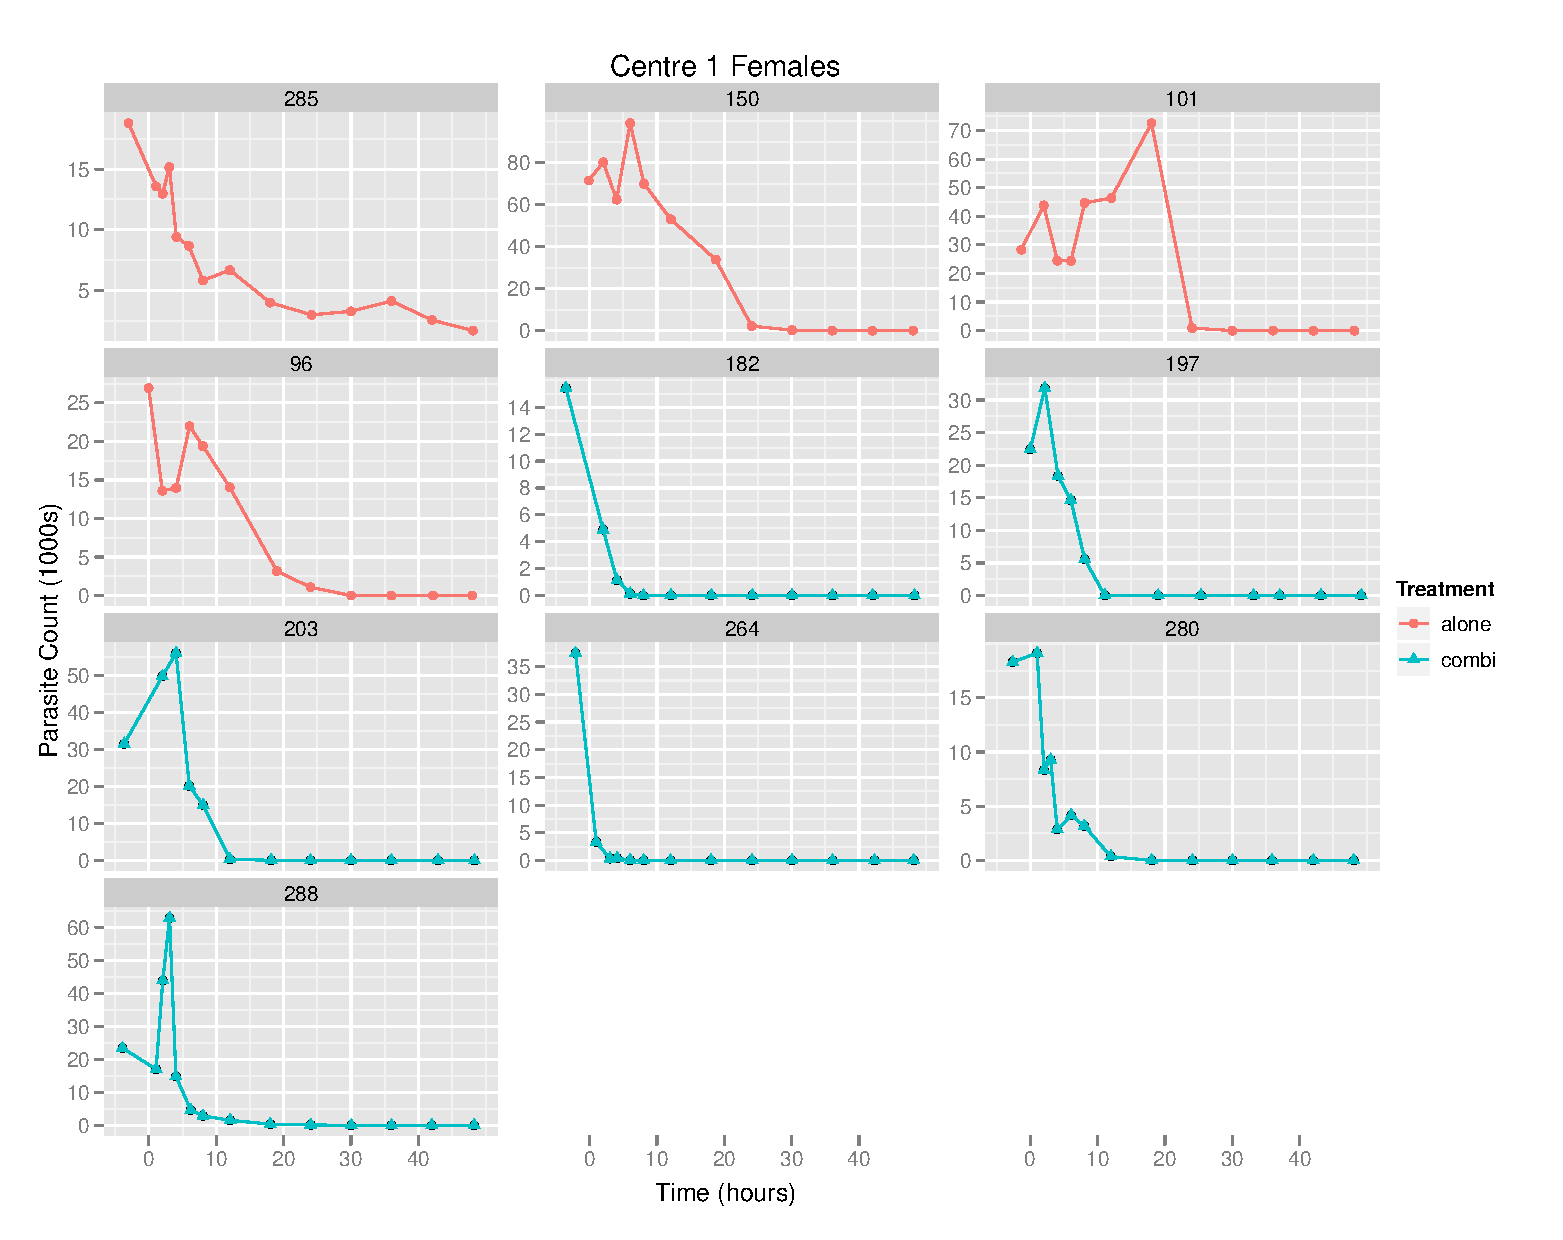
\includegraphics[width=6.1in]{raw1f.eps}
\caption{Parasite count for centre 1 females}\label{raw1F}
\end{figure} 
\begin{figure}[h]
\centering
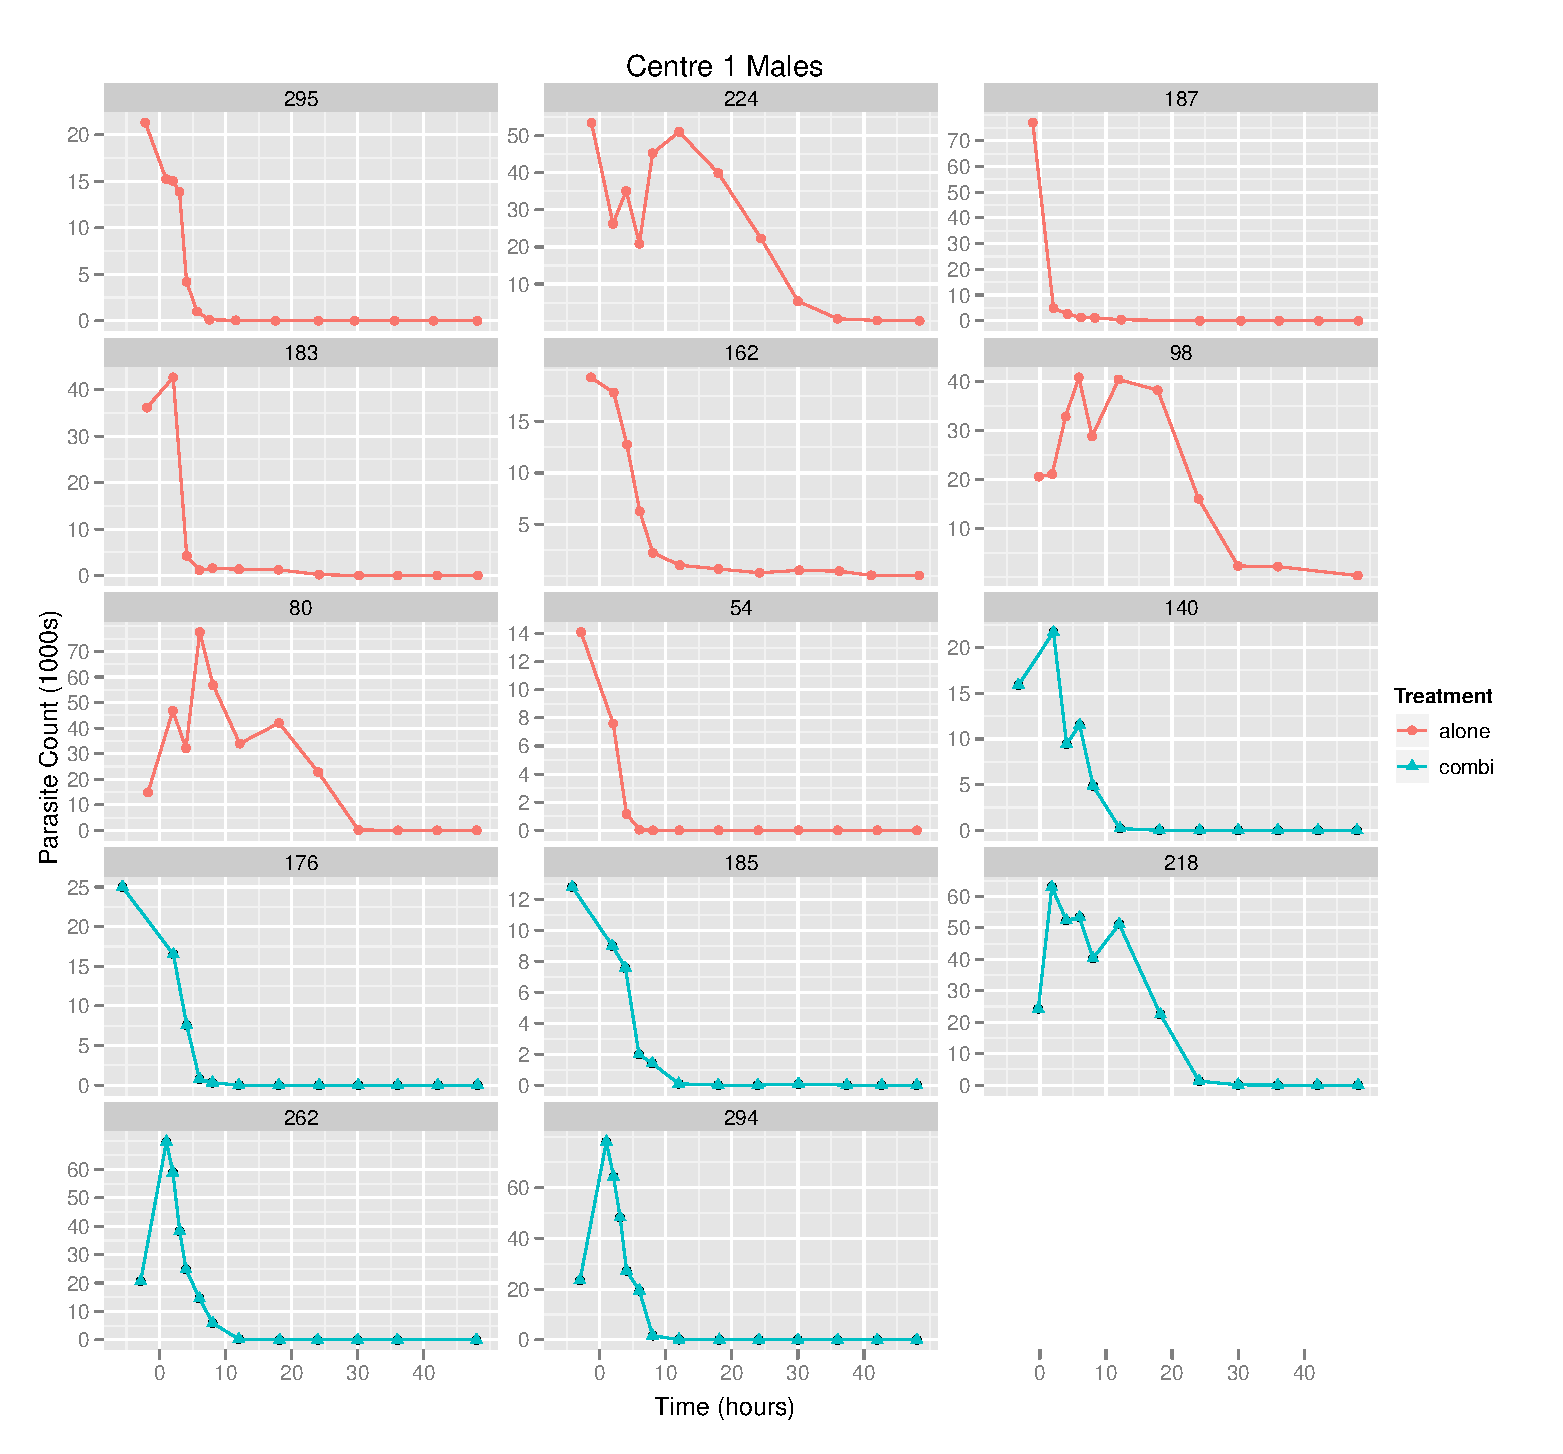
\includegraphics[width=6.1in]{raw1m.eps}
\caption{Parasite count for centre 1 males}\label{raw1M}
\end{figure} 
\begin{figure}[h]
\centering
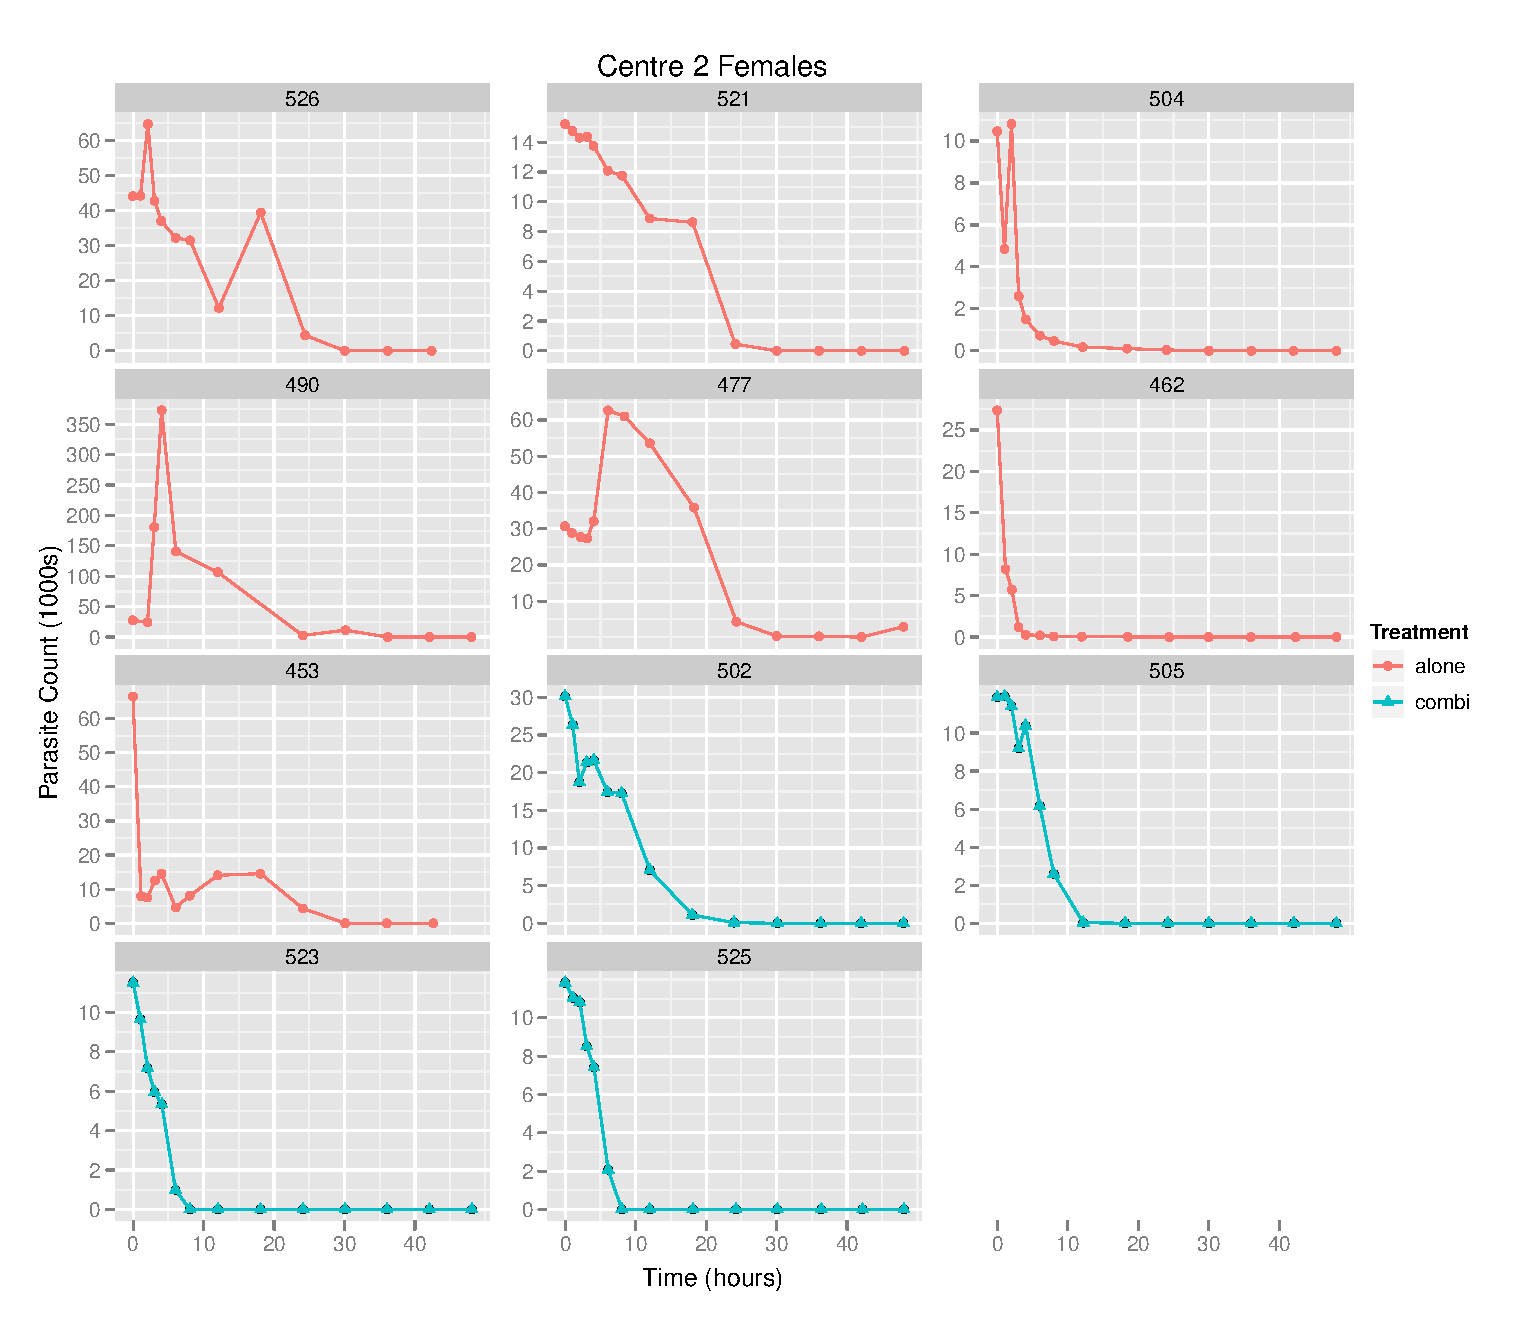
\includegraphics[width=6.1in]{raw2f.eps}
\caption{Parasite count for centre 2 females}\label{raw2F}
\end{figure} 
\begin{figure}[h]
\centering
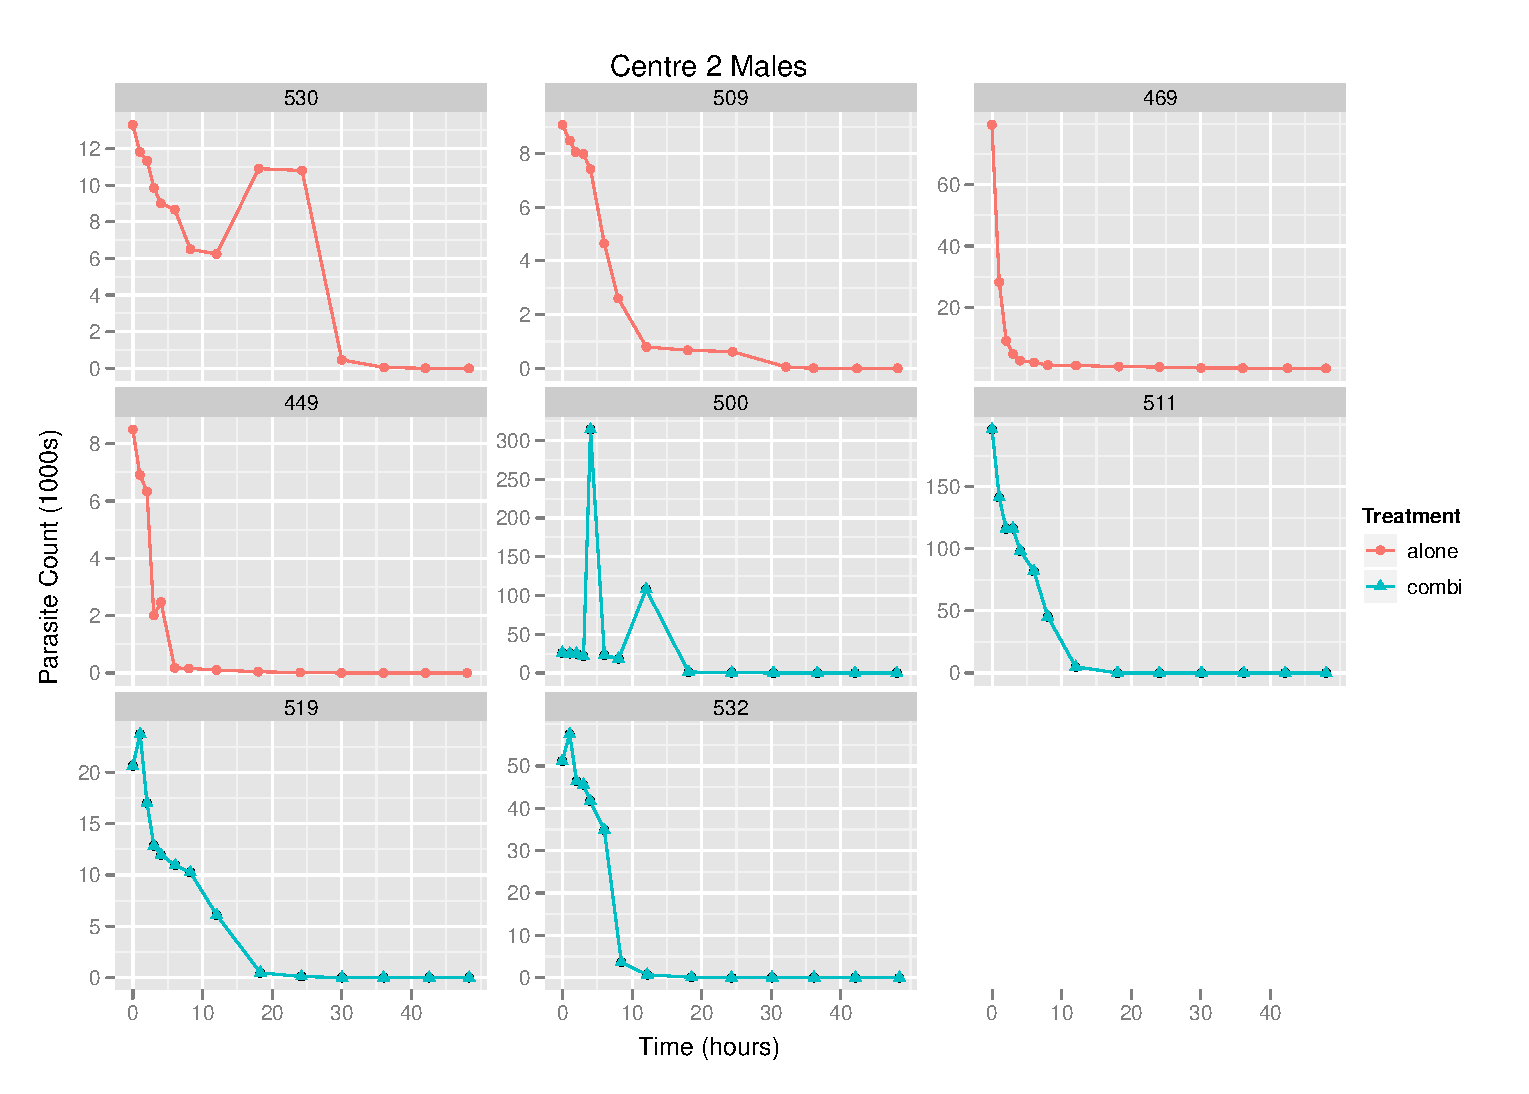
\includegraphics[width=6.1in]{raw2m.eps}
\caption{Parasite count for centre 2 males}\label{raw2M}
\end{figure} 
\subsection{Main features of the data}
Generally, there appears to be a drop in the parasite count from an initial high level to zero or near zero within about 20 to 30 hours from first treatment. In some cases there is a rapid monotonic drop off within 10 hours. In other cases the \textit{recorded} parasite count fluctuates up and down before dropping to zero over a longer period.

\pagebreak
To briefly summarise, the main behaviours observed are:
\begin{itemize}
\item A relatively steep monotonic drop in the count e.g. centre 1 female subjects 182 and 264 (Figure \ref{raw1F}), centre 1 male subjects 187, 162, 54, 176 and 185 (Figure \ref{raw1M}), centre 2 female subjects 462, 523 and 525 (Figure \ref{raw2F}) and centre 2 male subjects 509, 469 and 511 (Figure \ref{raw2M}).

A variation of this type comprises has the parasite count increasing after the first dose before falling e.g. subjects 197 and 203 (Figure \ref{raw1F}) and subjects 262 and 294 (Figure \ref{raw1M}). 
\item A more erratic and slower drop in the parasite count e.g. centre 1 female subjects 285 and 96 (Figure \ref{raw1F}), centre 1 male subjects 295 and 140 (Figure \ref{raw1M}) and centre 2 female subjects 521, 502 and 505 (Figure \ref{raw2F}). 
\item The parasite count seems to fluctuate about a constant level before falling e.g. centre 1 female subjects 150 and 101 (Figure \ref{raw1F}) and centre 1 male subjects 224, 98, 80 and 218 (Figure \ref{raw1M}). 
\end{itemize}
There are some profiles that we might suspect contain anomalous data such as subject 500 in Figure \ref{raw2M} where there are two unusually high values compared to the main trend. We might suspect that some inconsistency in the counting procedure explains these values rather than the patient's parasite count jumping by a large amount on these occasions. Looking at how the parasite count was obtained should give an insight into potential sources of inconsistency.
\section{Derivation of the Parasite Count}
One of the first questions addressed was whether the parasite count is a true count, and thus Poission statistics would be applicable, or whether it is a derived measurement. Our contact informed us that the method used to arrive at the parasite count values given is broadly as follows.
\begin{enumerate}
 \item A microscopist would choose ``suitable area'' of a slide of blood and work from left to right counting parasites ($N_p$) and white blood cells ($N_w$).
\item If by the time they have counted around 200 white blood cells they have seen less than 10 parasites then they continue counting until they have counted around 500 white blood cells.
\item The number of white blood cells in a $\mu L$ of blood ($\rho_w$) is automatically counted by a machine.
\end{enumerate}
Accordingly the number of parasites in a $\mu L$ of blood (\texttt{parct}) is given by:
$$\mathtt{parct}=\frac{N_p}{N_w}\rho_w$$
and thus we cannot treat this derived measurement as a count for modeling purposes.
\subsection{The Pre-dose parasite count}
We were also informed that the white blood cell count is right skewed and so we might expect that the parasite count per $\mu L$ will be also.
%Table \ref{predose} shows the pre-treatment parasite counts in the subjects from each test centre and of each sex. It can be seen that for 3 cases the mean is larger than the median meaning that the distributions are right skewed. This is to be expected for non-negative data such as this. When model fitting to this data we may have to choose some transformation of the parasite count such as taking logarithms.
Figure \ref{preaov} shows the pre-dose parasite counts grouped by sex, centre and treatment. There does not seem to be an obvious dependence of the level of the pre-dose parasite count on sex, centre or treatment. However, it does seem as if female pre-dose parasite count shows a higher dispersion than for males.

If we perform 3-way ANOVA of the pre-dose parasite count with sex, centre and treatment we find that there is no evidence of a dependence on these factors. The Kruskal-Wallis non-parametric equivalent test also does not reveal any evidence of a dependence. 
\begin{table}[h]
\centering
\caption{Pre-dose parasite counts}\label{predose}
\begin{tabular}{|cc|cccccc|}
\hline
Centre&Sex&N&Mean&Median&SD&1st Qu.&3rd Qu.\\\hline
\multirow{2}{*}{001}&M&14&27060&20960&17820.9&16750&24830\\
&F&10&29410&25170&16221.2&19700&30700\\\hline
\multirow{3}{*}{002}&M&8&50540&23290&63679.9&12240&58290\\
%&$M^*$&\textit{7}&\textit{29750}&\textit{20610}&\textit{26436.6}&\textit{11180}&\textit{38580}\\
&F&11&26110&27360&17262.4&11860&30400\\\hline
\end{tabular}
\end{table}
\begin{figure}
\begin{center}
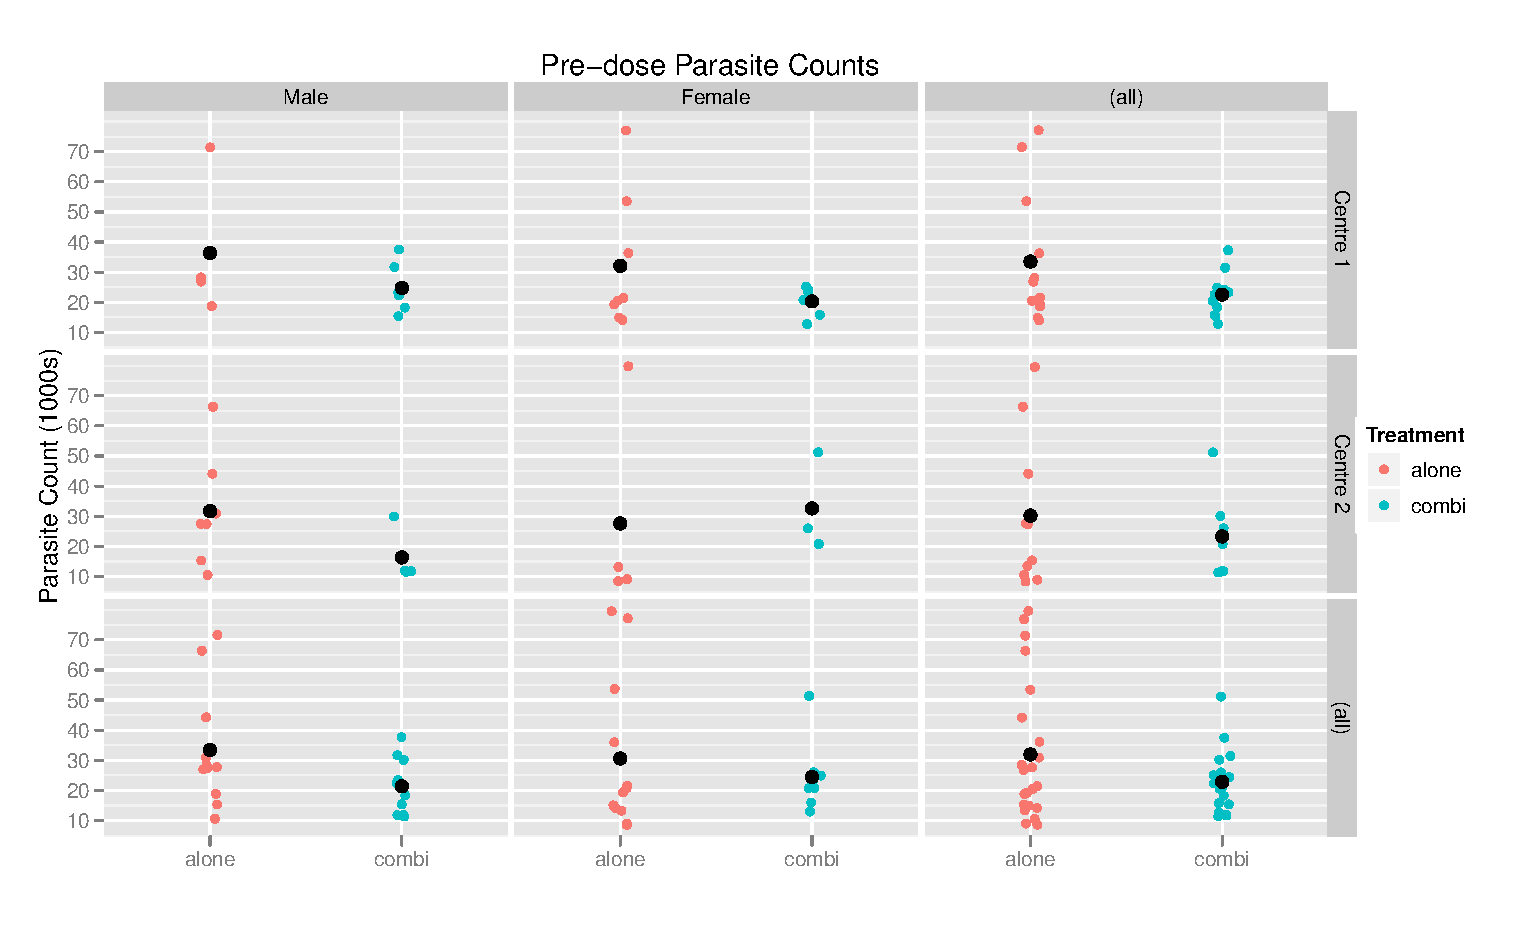
\includegraphics[width=6.1in]{preaov.eps}
\caption{Pre-dose parasite counts by sex, centre and treatment with mean shown. The right-hand column of panels shows both sexes combined grouped by centre; the bottom row shows both centres combined, grouped by sex and the bottom-right corner panel shows both sexes and centres combined.}
\label{preaov}
\end{center}
\end{figure}
\begin{sidewaysfigure}[p]
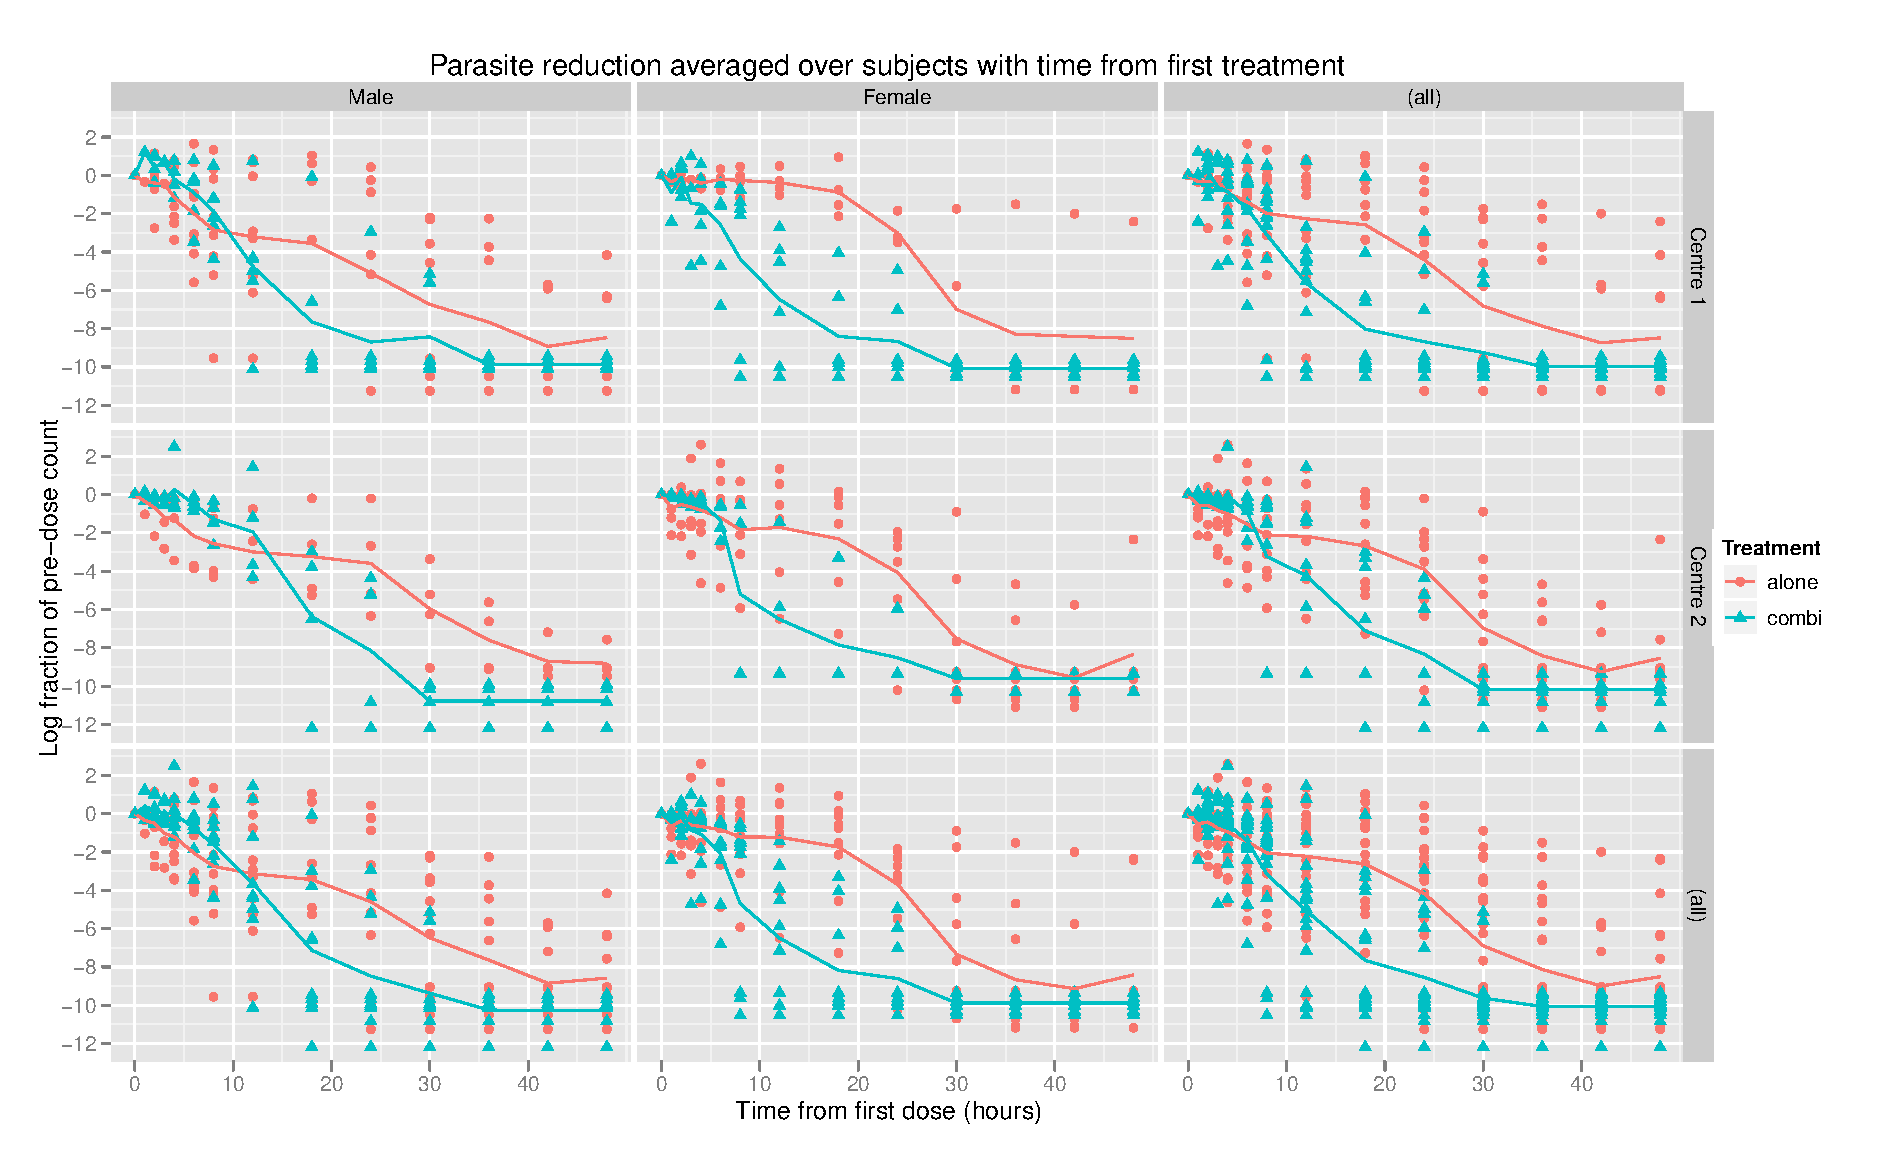
\includegraphics[width=9.2in]{allaov.eps}
\caption{ }
\label{ }
\end{sidewaysfigure}

\chapter{Derivation of Parasite Clearance Times}
\section{Estimating the primary endpoint}
The endpoint of primary importance is PC90, the time to achieve a reduction of the parasitaemia by 90\% of baseline level. The baseline level is the pre-dose parasite count. We have data for parasite counts taken at specific times and therefore will have a measurement of the parasite count at a time when the count was above 90\% of the baseline, followed by one where it where it is below 90\% and hence we need to find an appropriate interpolation to determine a time at which the parasite count was 90\%.

As a first attempt at deriving estimates of PC90 from the data, simple linear polynomial fits to the logarithm of the parasite count with time from first dose are investigated. This is followed by non-linear logistic regression as has been used by others\cite{wootton}. We also look at simple linear or or log-linear interpolation which has also been used for data of this kind\cite{carmello}.
\subsection{Using a transformation of the count}
In the previous chapter it was noted that a logarithmic transformation was appropriate to remove the skew of the parasite count distribution. Figure \ref{raw901M} shows the untransformed parasite count for centre 1 males with a horizontal line indicating the PC90 level and Figure \ref{log901M} shows the log-transformed parasite count.

We can see that the logarithmic transformation reduces the significance of large fluctuations in the parasite count soon after first dose and brings the region around the PC90 level into greater prominence. Consequently, interpolated estimates of PC90 in these log-linear co-ordinates will be more accurate and any regression will be more influenced by data close to the region of interest.  
\begin{figure}[p]
\begin{center}
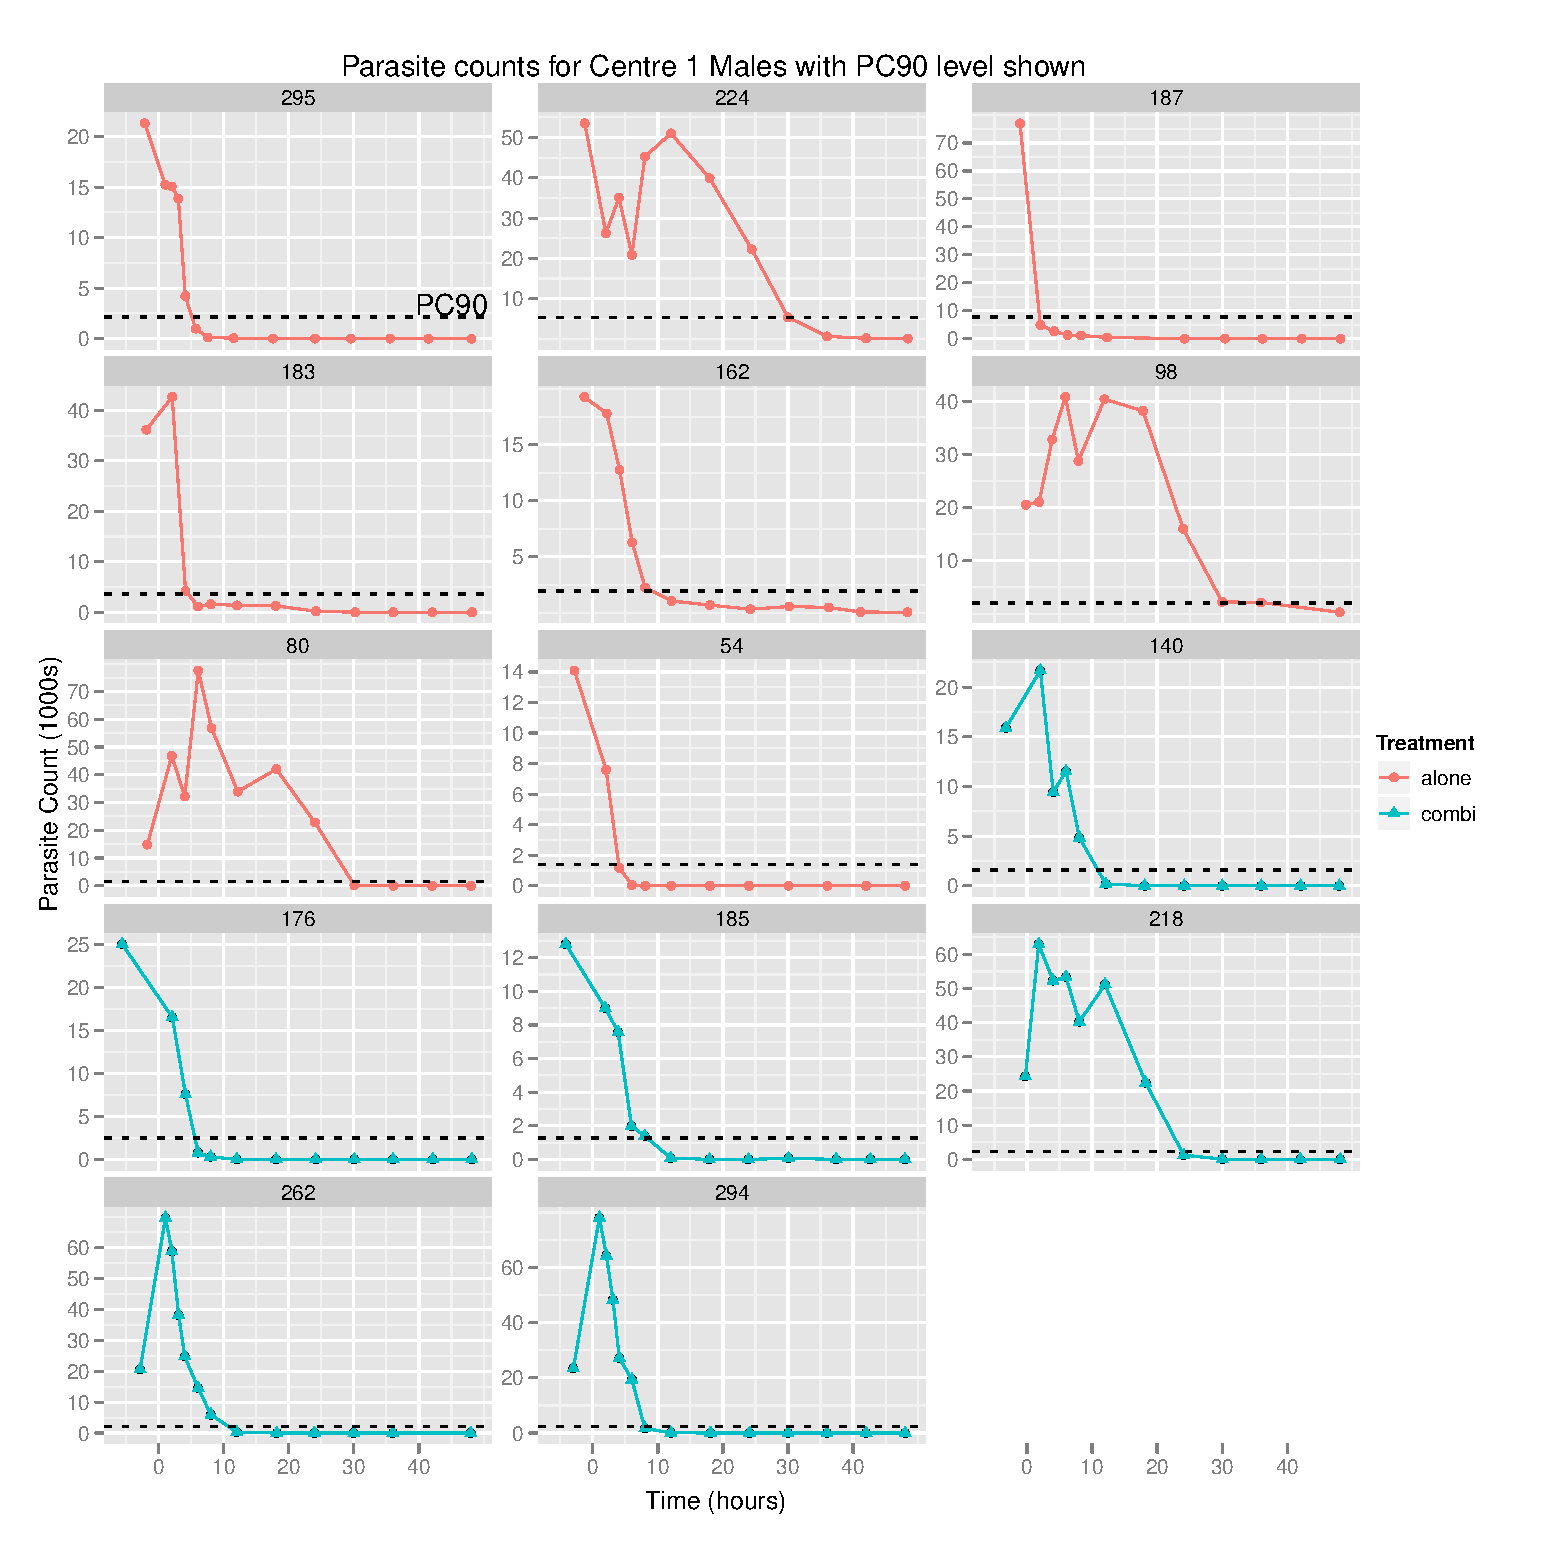
\includegraphics[width=6.1in]{raw901M.eps}
\caption{Untransformed parasite counts with PC90 level shown}
\label{raw901M}
\end{center}
\end{figure}
\begin{figure}[p]
\begin{center}
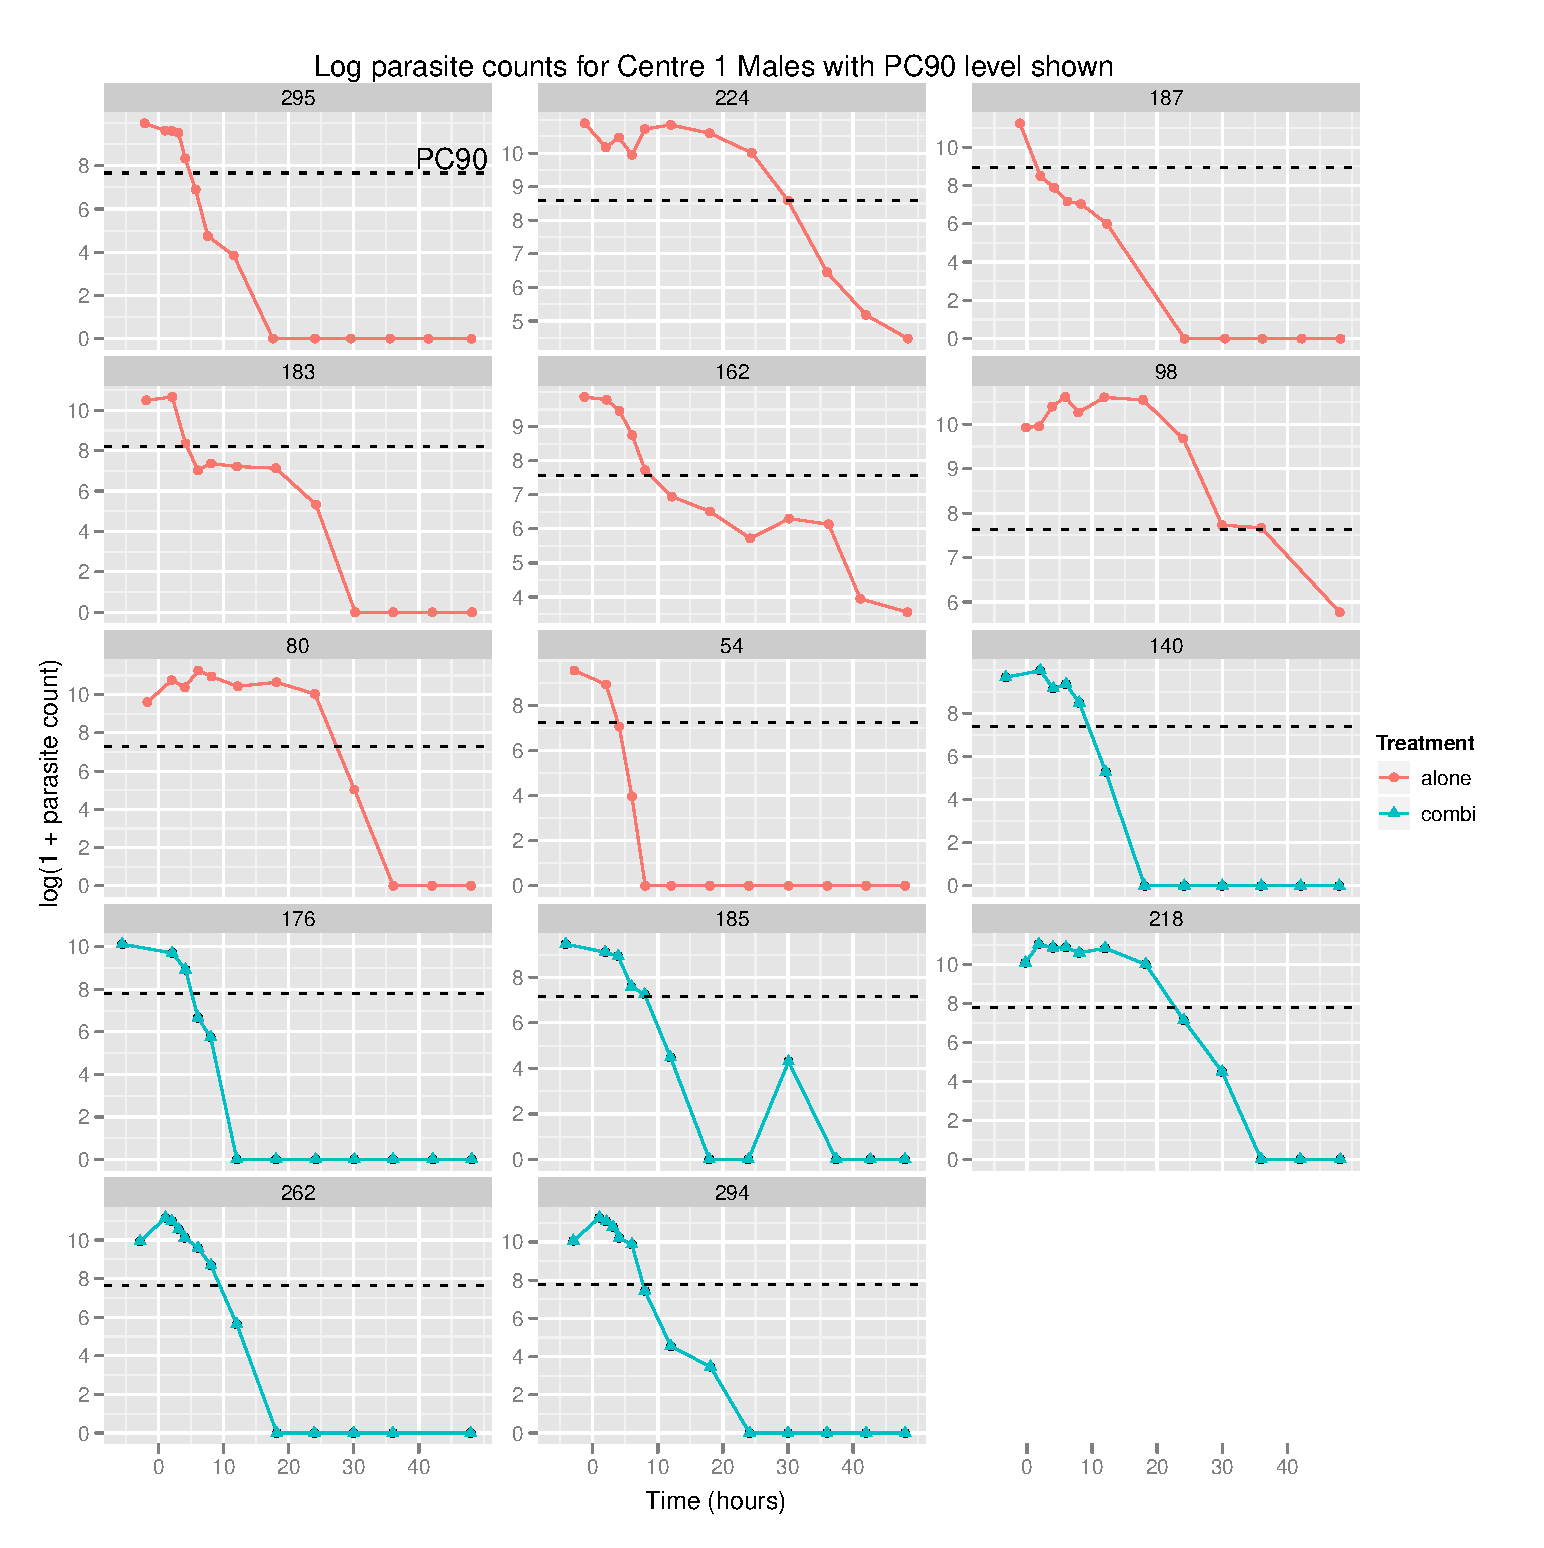
\includegraphics[width=6.1in]{log901M.eps}
\caption{Log parasite counts with PC90 level shown}
\label{log901M}
\end{center}
\end{figure}
\section{Estimation techniques}
\subsection{Polynomial linear regression}
It was found that a cubic was the most suitable model, if we include the data only up to the first 0 parasite count. For some patients where the parasite count drops quickly to 0 a fit that includes the subsequent run of 0s would pull the cubic fit away from the most sensible estimate of PC90. It is more suitable for the purpose of estimating PC90 to only model the drop in the count to 0.

A cubic model was fitted to the log-transformed parasite count $P_{t}$ with time from first dose $t$ as the explanatory variable
$$\log(1+P_{t})=\beta_0+\beta_1t+\beta_2t^2+\beta_3t^3+\epsilon\quad\quad\epsilon\sim N(0,\sigma^2)$$

Figure \ref{cubics} shows the cubic fits to the log parasite count for centre 1, male subjects. It can be seen that the model describes the data fairly well, but it looks as if the combined treatment data is more closely modelled with the single treatment data showing more dispersion about the fitted model. 
\begin{figure}[p]
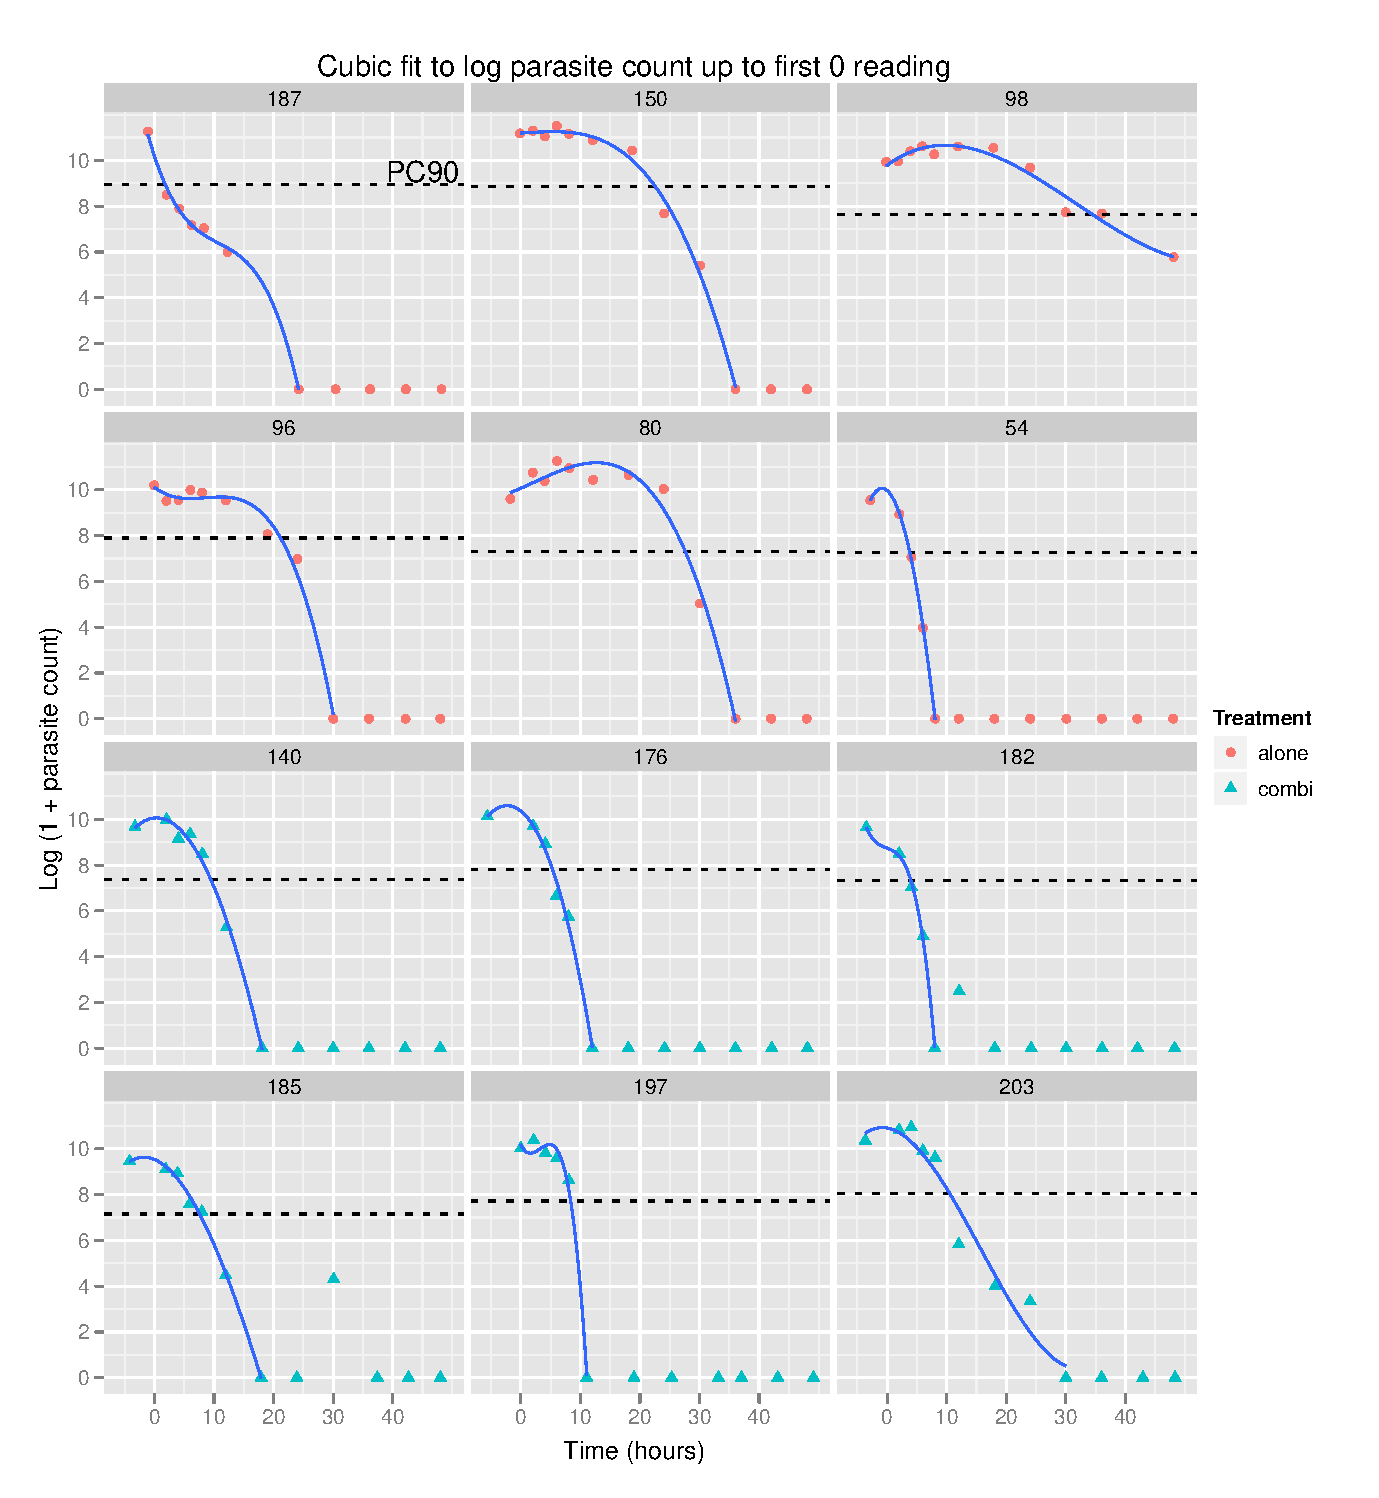
\includegraphics[width=6.1in]{cubics.eps} 
\caption{Cubic fits to log parasite count up to first zero reading}\label{cubics}
\end{figure}

Figure \ref{cubicsresid} shows the standardized residuals ($e/\hat{\sigma}$) for the cubic fits.
\begin{figure}[h]
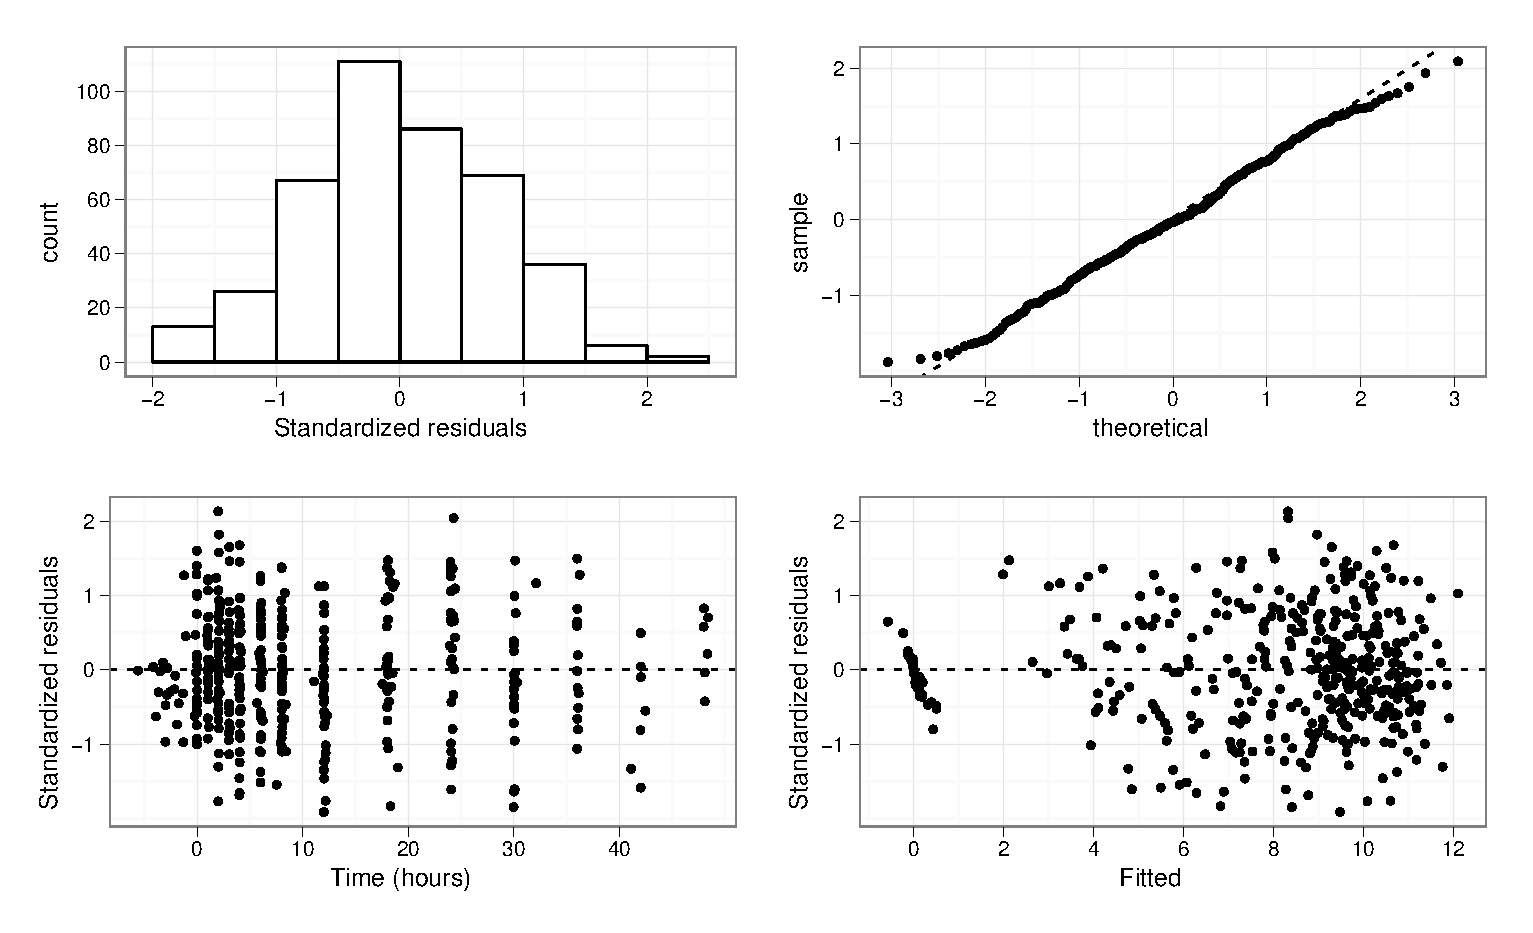
\includegraphics[width=6.1in]{cubicsresid.eps} 
\caption{Standardized residuals for cubic fits}\label{cubicsresid}
\end{figure}
It can be seen that they are normally distributed and show no obvious correlation with time from first dose or with fitted count. The cluster of small magnitude residuals at 0 fitted value occurs because this datum in the fit for each subject is not random but is always 0. Strictly this invalidates the assumptions of the fitted model but there isn't a more suitable choice for determining the shape. The cubic model is really only used as a convenient method of interpolation and we are not interested in the accuracy of the fitted parameters as long as there is no systematic bias. 
\subsubsection*{Determining PC90 from the fitted model}
The value of PC90 i.e. the time t at which the parasite count has fallen to 10\% was found by finding the positive root of the cubic equation
$$\hat{\beta_0}-\hat{\beta_1}t-\hat{\beta_2}t^2-\hat{\beta}_3t^3-0.1{P_{0}}=0$$
that lies within our time period, where $P_0$ is the pre-treatment parasite count, $t$ is the time from first dose and $\hat{\beta_i}$ are the fitted coefficients for the cubic model. This root was found numerically using the \emph{R} \texttt{uniroot} function which takes as an argument the interval over which to search for the root.
\pagebreak
\subsection{Non-linear logistic regression}
The logistic model fitted is
$$\log(1+P_t)=\alpha+\frac{\lambda}{1+e^{-\beta(t-\mu)}}+\epsilon$$
This was fitted to all the data as it can model a drop from an initial count level to a level of 0, unlike the cubic model. $\alpha$ is the lower asymptote which we would expect to be 0. $\alpha+\lambda$ is the upper asymptote which we would generally expect to be $P_0$ except in the cases where there is a marked increase in the parasite count after the first dose. $\beta$ determines the rate of reduction with time and $\mu$ is the point of inflection (maximum rate of reduction). This model was fitted using non-linear least-squares routines in \emph{R} and \emph{SAS}. Logistic fits to the same subjects as the cubic fits in Figure \ref{cubics} are shown in Figure \ref{logistics}.
\begin{figure}[p]
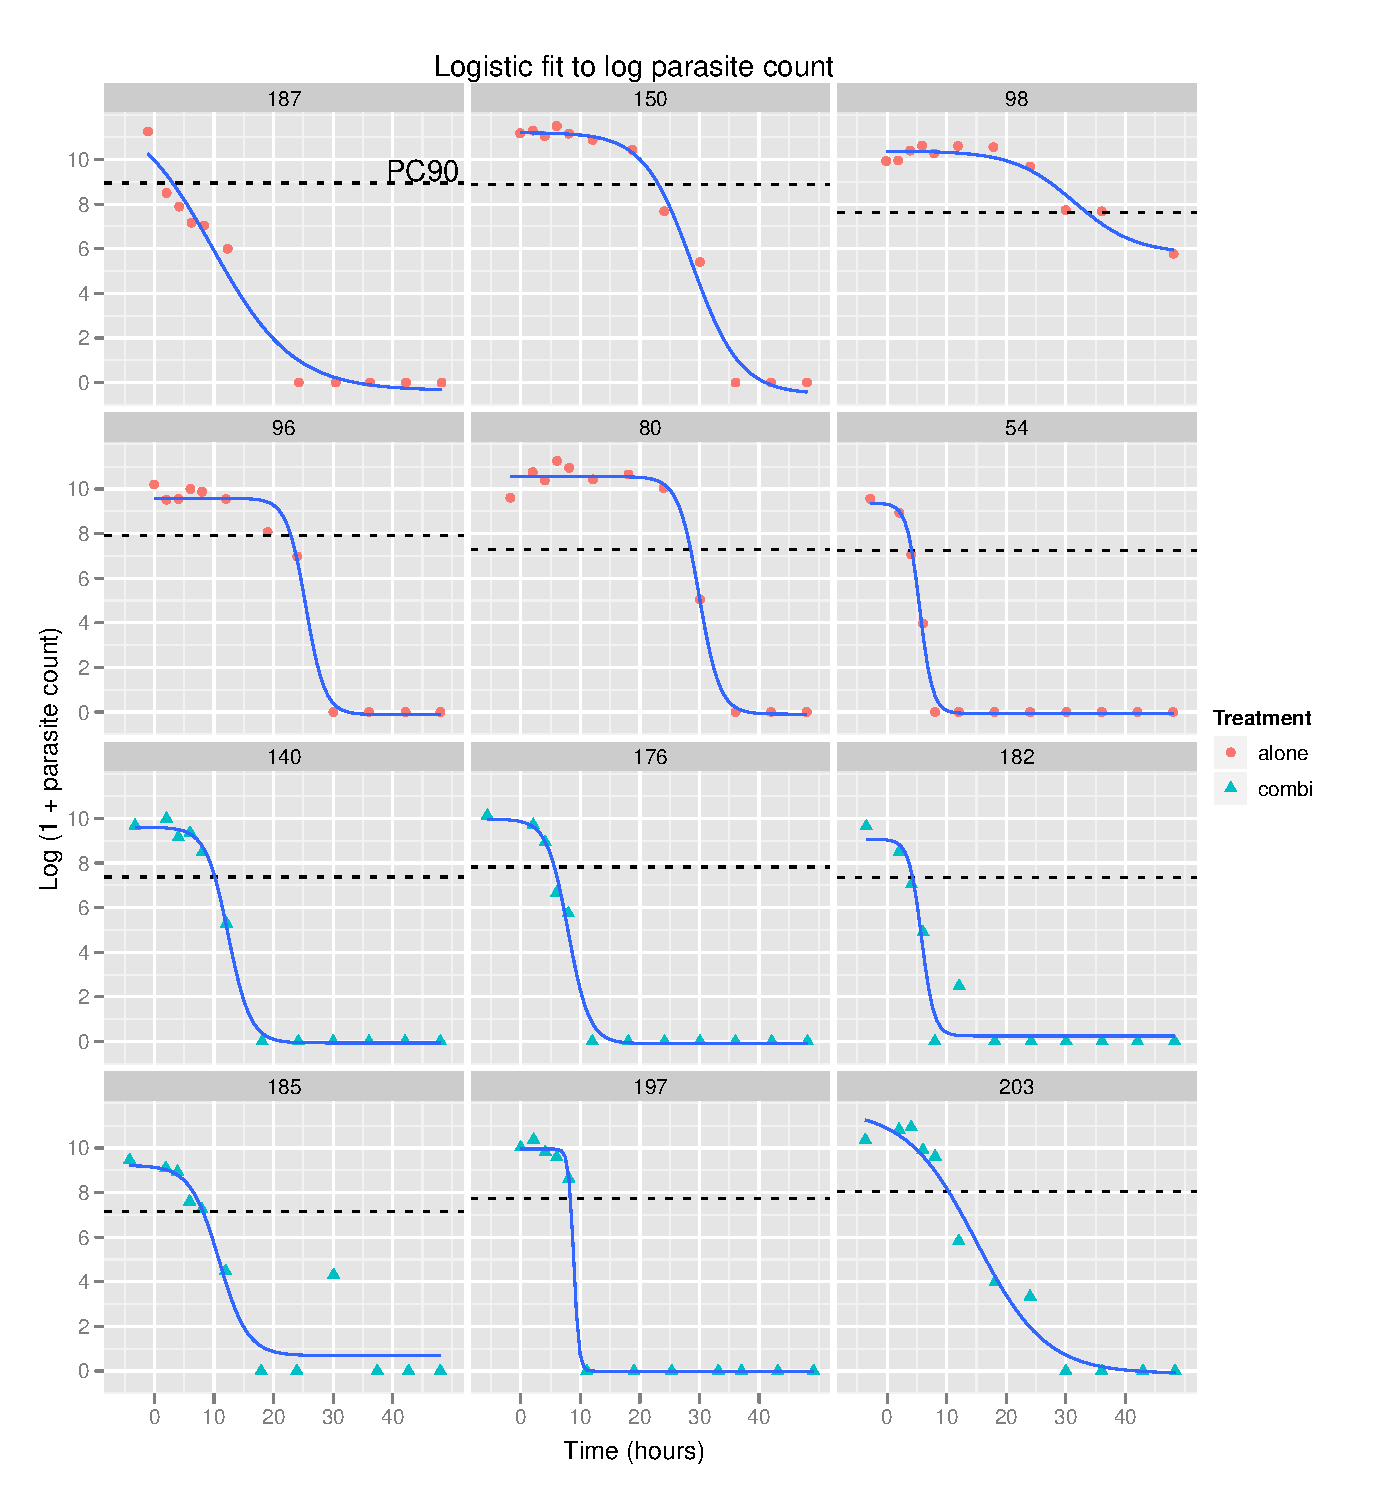
\includegraphics[width=6.1in]{logistics.eps} 
\caption{Logistic fits to log parasite count}\label{logistics}
\end{figure}
\pagebreak
\subsubsection*{Choosing starting values for the parameters}
Figure \ref{logparms} shows the roles the parameters of the logistic model play in shaping the fitted curve. The non-linear, least-squares fitting routines (the \texttt{nls} function) in \emph{R} can take starting values for the parameters to be estimated.
\begin{figure}[h]
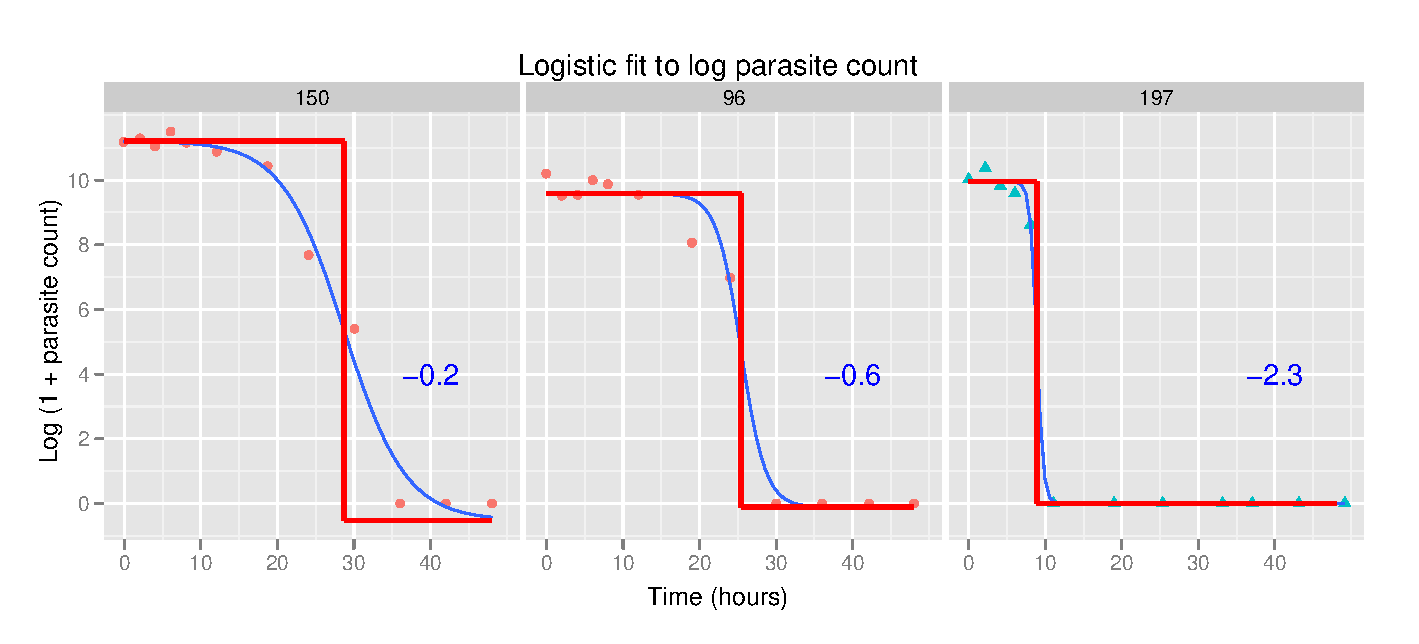
\includegraphics[width=6.1in]{logparms.eps} 
\caption{Illustration of parameters for logistic fits.\newline
The horizontal red lines show $\log(1+P_t)=\alpha$ (lower) and $\log(1+P_t)=\alpha+\lambda$ (upper), the vertical red line shows $t=\mu$ and the coefficient $\beta$ (rate of reduction) is given in blue.}\label{logparms}
\end{figure}

Looking at Figure \ref{logparms} it clearly follows that sensible starting values are:
\begin{itemize}
\item $\alpha$ = the minimum parasite count; usually 0.
\item $\lambda$ = the maximum minus the minimum count; usually the maximum.
\item $\mu$ = the time corresponding to the parasite count closest to halfway between the maximum and minimum counts.
\end{itemize} 
It was found by experimentation that the most suitable starting value for $\beta$ was -0.5, but that the fitting was insensitive to choice of $\beta$ if varied over the range of fitted $\beta$ values observed (and somewhat beyond).
\subsubsection*{Failure of logistic fitting}
Despite careful selection of starting parameters, it was found for several subjects that a logistic model is simply not appropriate. In these cases either the non-linear fitting routine failed to converge or, if convergence criteria were relaxed, would fit a model highly dependent on choice of starting parameters and when plotted with the data obviously does not model the data satisfactorily. The data for these subjects where logistic fitting failed are shown in Figure \ref{failures}.
\begin{figure}[h]
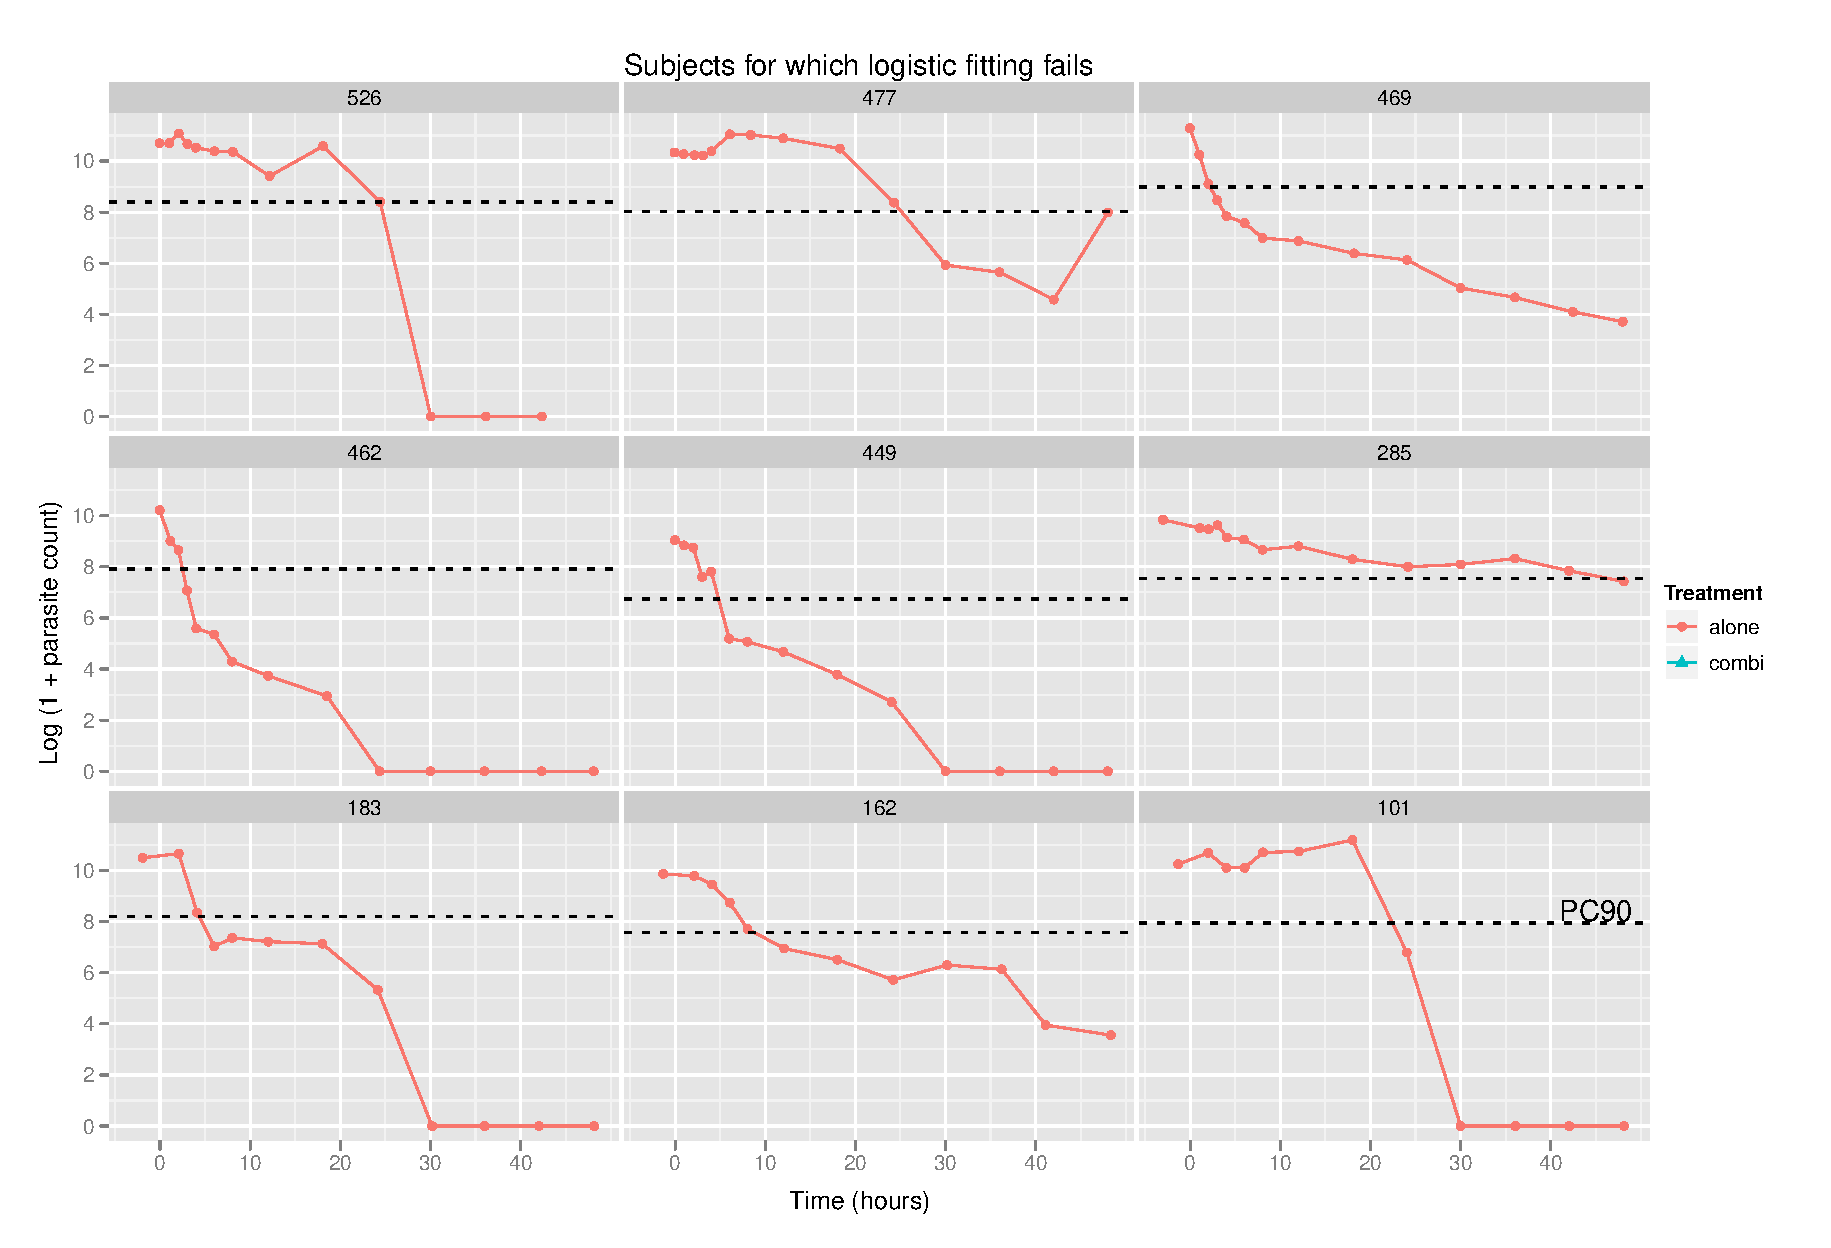
\includegraphics[width=6.1in]{failures.eps} 
\caption{Subjects for which the logistic fitting fails}\label{failures}
\end{figure}

It is interesting to note that all subjects for which logistic fitting fails are in the single treatment group; $p=0.0039$ under the null hypothesis of equal probability of a subject being from the single or combined treatment group using a binomial model. This is evidence that the parasite counts for patients on the single treatment follow more varied trajectories during clearance compared to patients on the combined treatment whose clearance can consistently be described with a logistic model to a good approximation. This was also the case for the cubic model.

In addition to parasite count profiles that simply do not conform to a logistic shape there were subjects where insufficient data in the region between the upper and lower asymptotes meant that logistic fitting was inappropriate. For example subjects 526 and 101 in Figure \ref{failures} where choice of different starting parameters for $\mu$ and $\beta$ would result in different logistic fits being obtained. One possible fit having a steep transition (large absolute $\beta$) whereby the data at the upper and lower levels is closely modeled. Another possible fit having a shallower transition (smaller $\beta$) that models the slope of a line passing through the ends of the run of points at the upper and lower levels and the point in the middle, but that has a less severe curvature such that the corners at the upper and lower levels are less well modeled. In summary the fit is free to rotate about the single point between the upper and lower levels and thus cannot be suitably defined.
\subsection{Log-linear interpolation}
The datum immediately above the PC90 level is joined with a straight line to the datum immediately below the PC90 level in on a plot of $\log(1+P_{t})$ against time. The point where this line crosses the PC90 level determines $t$=PC90.
\section{Comparison of estimation methods}
\subsection{Graphical comparison}
Figure \ref{pc90-agree} shows 8 examples of subjects where estimation by the 3 different methods shows good agreement. It seems likely that the differences between these estimates are comparable to experimental error. It can be seen that the 3 methods give close agreement when the data can be closely modeled by cubic or logistic fitting and when the gradient of the log-linear interpolation is similar to the regression models in the region around PC90. 
\begin{figure}[h]
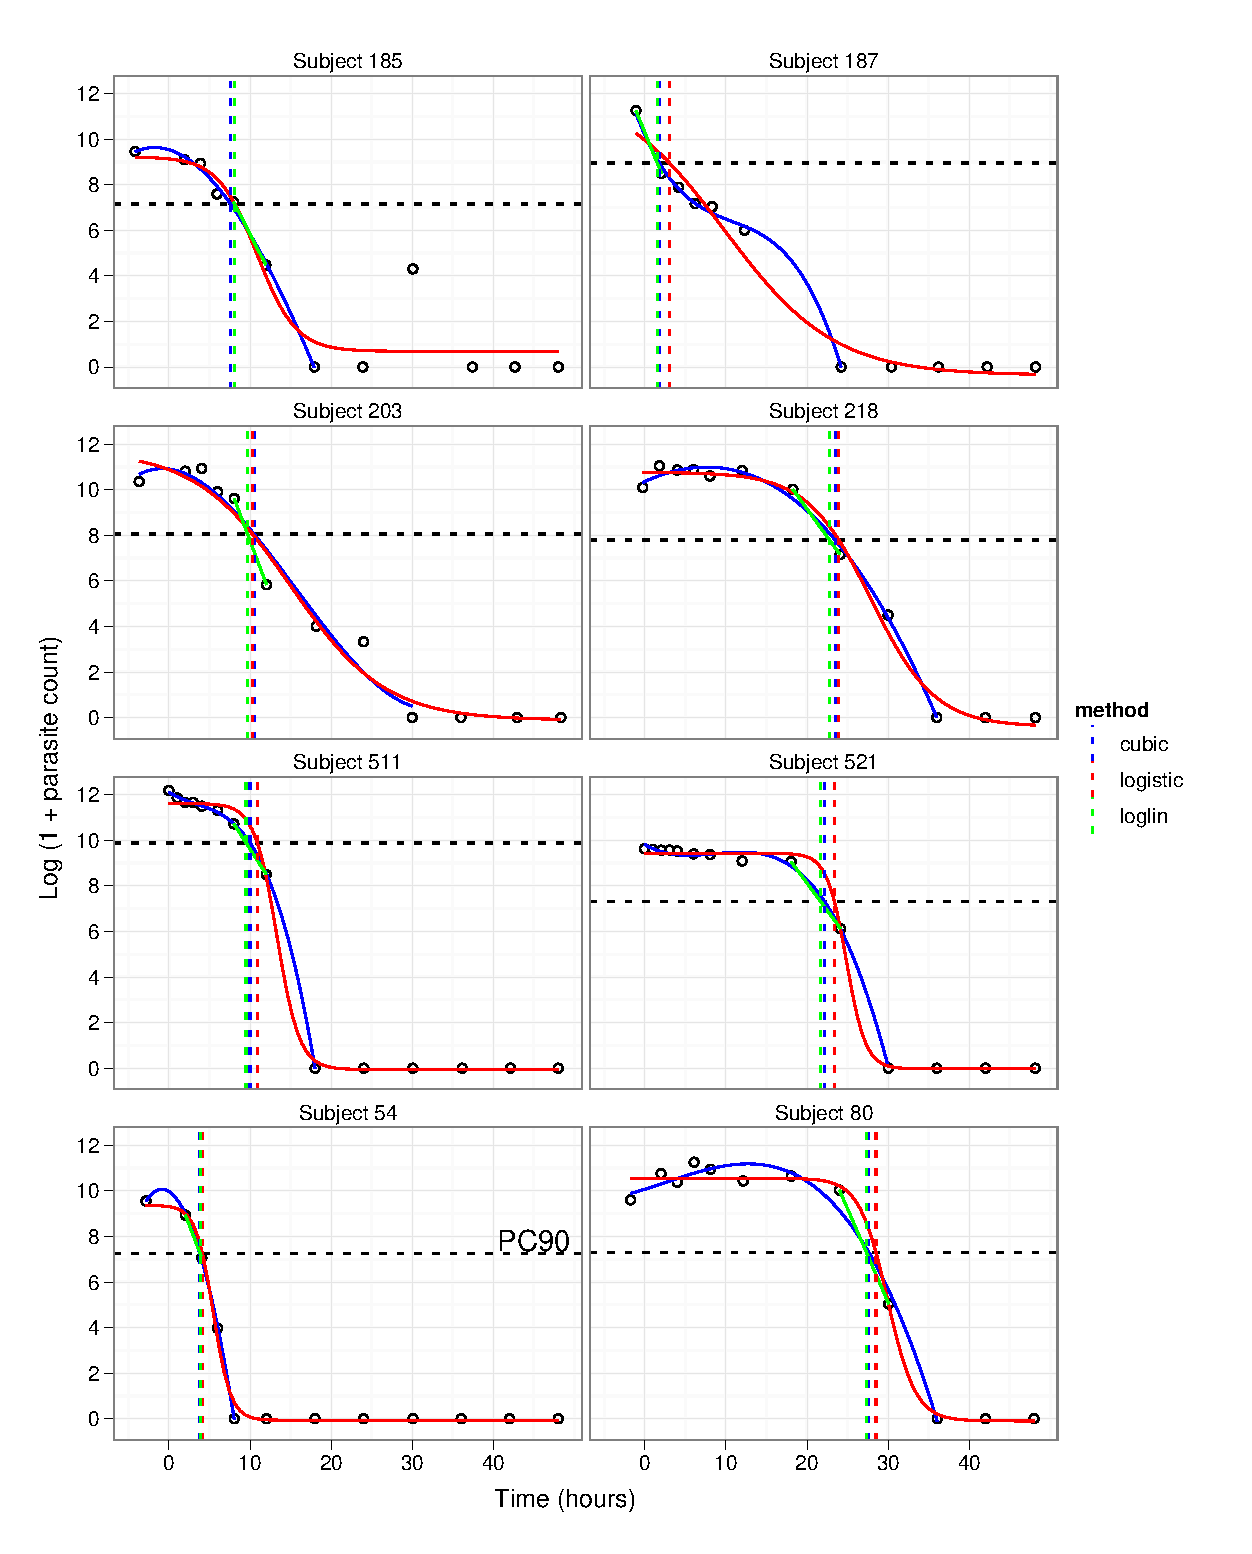
\includegraphics[width=6.5in]{pc90-agree.eps} 
\caption{Subjects with little difference in PC90 estimated by 3 methods}
\label{pc90-agree}
\end{figure}

Figure \ref{pc90-bad} shows examples of subjects where estimation by the 3 different methods has resulted in notable differences between PC90 estimates. These differences appear to arise when:
\begin{enumerate}
\item The drop in parasite count is slow or stationary around the PC90 level e.g. subjects 98, 453 and 509. In these cases the regression lines and interpolation may cross the PC90 level at markedly different times. In subject 509 this has given a difference in PC90 between the interpolation and cubic methods of almost 10 hours.
\item There is ``unusual'' data near the PC90 level e.g. subjects 490 and 500 where recorded counts seemingly off the prevailing trend have influence the interpolated estimate.
\end{enumerate}
\begin{figure}[h]
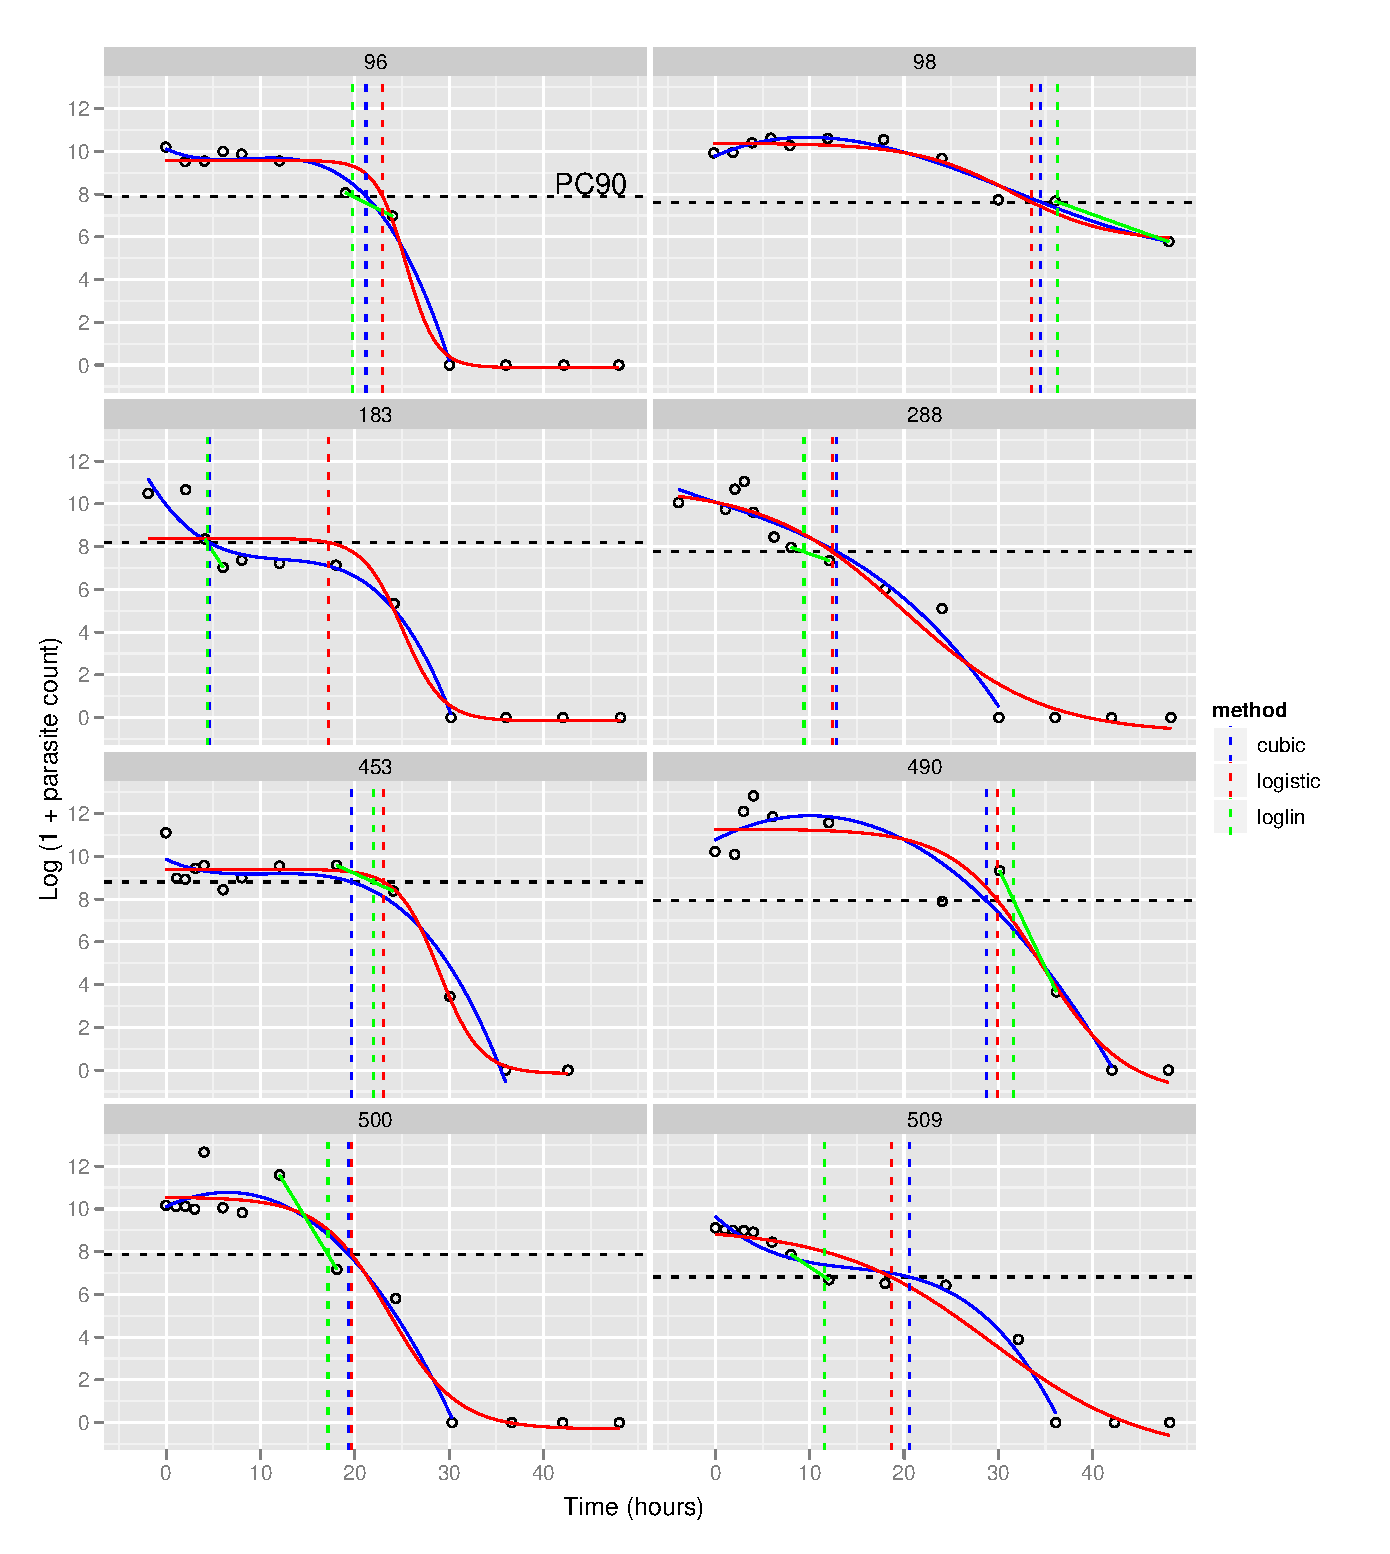
\includegraphics[width=6.5in]{pc90-bad.eps} 
\caption{Subjects with notable difference in PC90 estimated by 3 methods}
\label{pc90-bad}
\end{figure}
Figure \ref{pc90-nofit} shows the cubic and log-linear interpolated estimates for subjects where logistic fitting was innapropriate.
\begin{figure}[h]
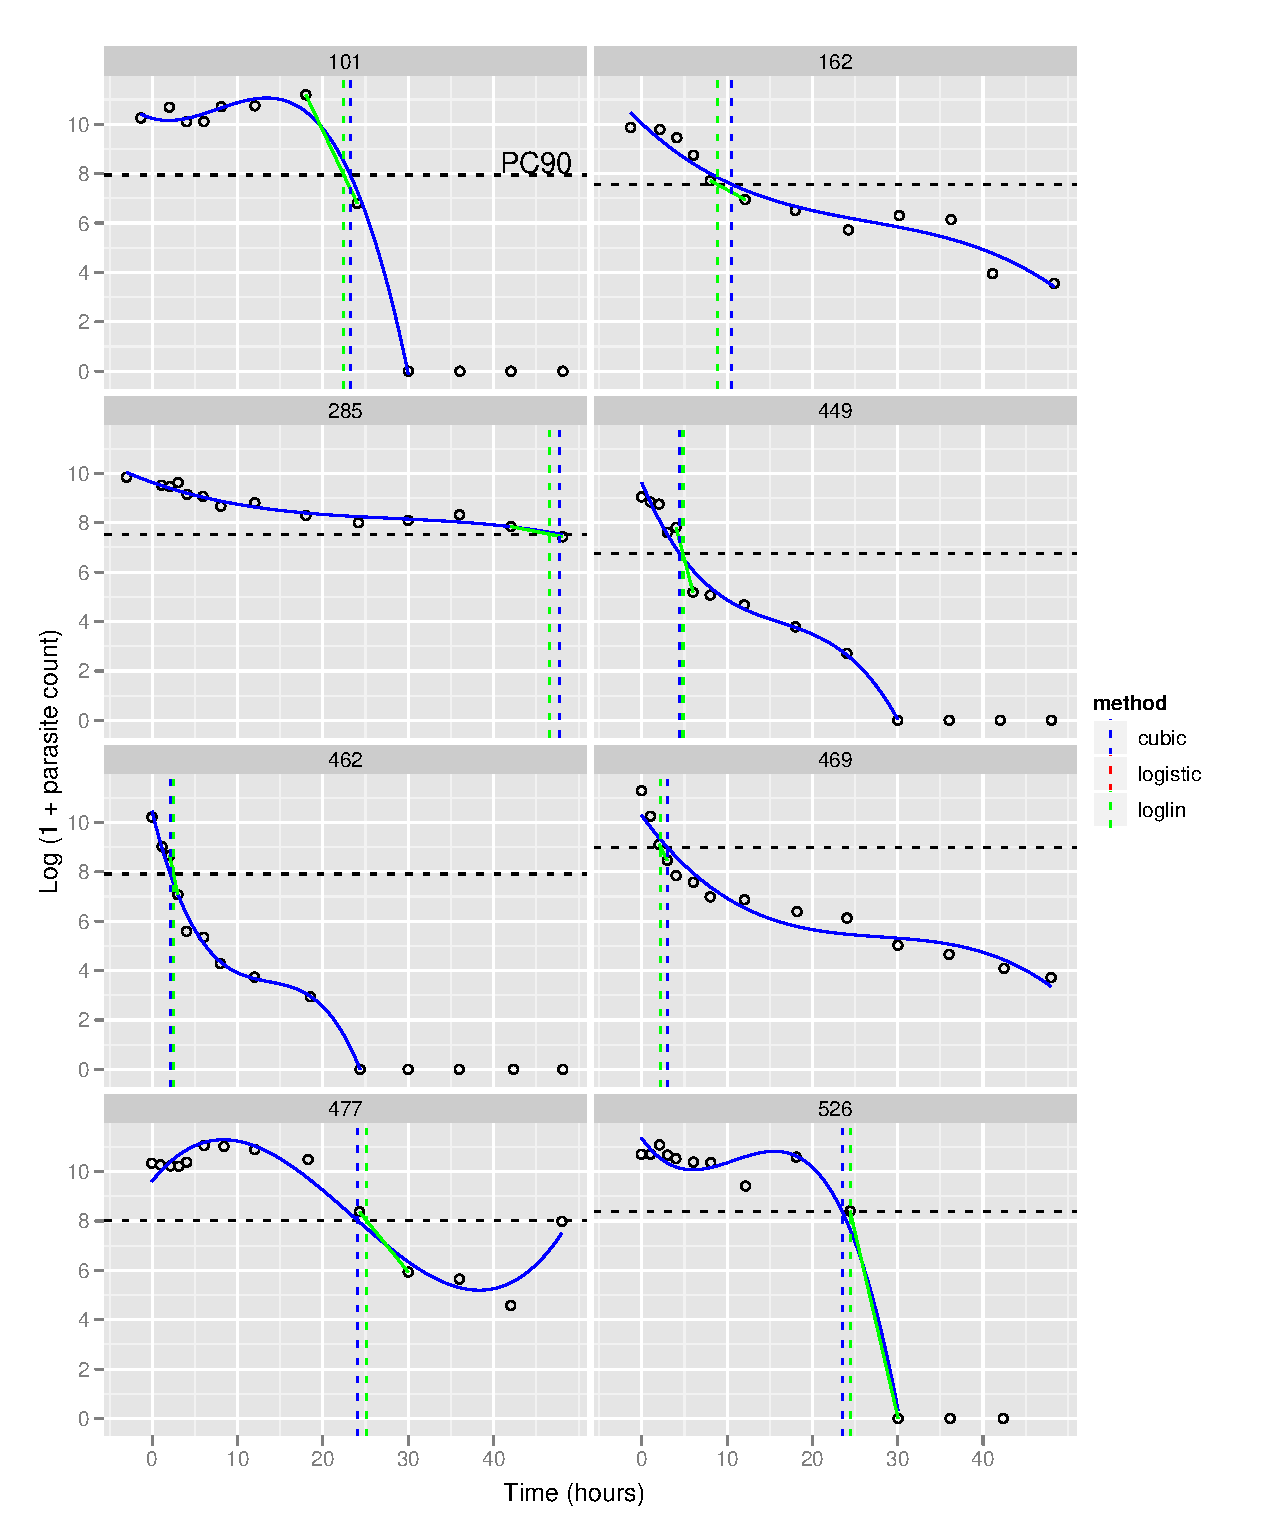
\includegraphics[width=6.5in]{pc90-nofit.eps} 
\caption{PC90 estimation for subjects where logistic fitting was inappropriate}
\label{pc90-nofit}
\end{figure}
It can be seen that the two methods in these cases appear to produce very similar estimates.
\clearpage
\subsection{Statistical comparison}
Table \ref{PC90} shows a comparison of the PC90 estimates by the 3 different methods utilised so far.
\begin{table}
\centering
\caption{Comparison of PC90 estimated by 3 methods}\label{PC90}
\begin{tabular}{|cccc|rrr|}
\hline
Subject&Centre&&&PC90&PC90&PC90\\
ID&ID&Sex&Treatment&cubic&logistic&log-linear\\
\hline
54&Centre 1&Male&alone&3.82&4.14&3.85\\
80&Centre 1&Male&alone&27.62&28.50&27.32\\
96&Centre 1&Female&alone&21.18&22.95&19.76\\
98&Centre 1&Male&alone&34.50&33.51&36.30\\
101&Centre 1&Female&alone&23.20&-&22.45\\
140&Centre 1&Male&combi&9.47&10.16&9.47\\
150&Centre 1&Female&alone&22.52&23.12&21.75\\
162&Centre 1&Male&alone&10.54&-&8.84\\
176&Centre 1&Male&combi&5.32&5.66&5.05\\
182&Centre 1&Female&combi&3.98&4.29&3.65\\
183&Centre 1&Male&alone&4.55&17.21&4.35\\
185&Centre 1&Male&combi&7.59&8.13&8.10\\
187&Centre 1&Male&alone&1.81&3.05&1.53\\
197&Centre 1&Female&combi&8.38&8.35&8.40\\
203&Centre 1&Female&combi&10.48&10.30&9.69\\
218&Centre 1&Male&combi&23.48&23.92&22.77\\
224&Centre 1&Male&alone&28.86&30.26&30.01\\
262&Centre 1&Male&combi&9.40&9.85&9.40\\
264&Centre 1&Female&combi&0.37&1.43&0.85\\
280&Centre 1&Female&combi&8.76&9.72&9.04\\
285&Centre 1&Female&alone&47.74&-&46.52\\
288&Centre 1&Female&combi&12.86&12.38&9.38\\
294&Centre 1&Male&combi&8.86&8.68&7.73\\
295&Centre 1&Male&alone&5.02&4.98&4.83\\
449&Centre 2&Male&alone&4.45&-&4.82\\
453&Centre 2&Female&alone&19.66&23.08&21.97\\
462&Centre 2&Female&alone&2.11&-&2.49\\
469&Centre 2&Male&alone&3.01&-&2.21\\
477&Centre 2&Female&alone&24.03&-&25.08\\
490&Centre 2&Female&alone&28.73&29.94&31.63\\
500&Centre 2&Male&combi&19.36&19.66&17.15\\
502&Centre 2&Female&combi&15.33&16.33&14.77\\
504&Centre 2&Female&alone&5.07&6.64&5.00\\
505&Centre 2&Female&combi&8.26&9.02&8.75\\
509&Centre 2&Male&alone&20.59&18.63&11.59\\
511&Centre 2&Male&combi&10.00&10.91&9.51\\
519&Centre 2&Male&combi&15.63&16.08&14.68\\
521&Centre 2&Female&alone&22.14&23.38&21.64\\
523&Centre 2&Female&combi&5.82&5.97&5.84\\
525&Centre 2&Female&combi&6.15&6.17&6.23\\
526&Centre 2&Female&alone&23.48&-&24.42\\
530&Centre 2&Male&alone&29.10&29.28&28.09\\
532&Centre 2&Male&combi&9.16&9.21&8.08\\
\hline
\end{tabular}
\end{table}
%If we perform 2-way ANOVA between the 3 PC90 estimates by subject and method i.e.
%$$\mathrm{PC}90_{ij}=subject_{i}+method_{j}+\epsilon_{ij}\quad\quad\epsilon\sim N(0,\sigma^{2})$$ 
%we obtain the residuals shown in Figure \ref{pc90resid}.
%It can be seen that there are several outlying data points at up to $4\sigma$ and almost $8\sigma$. These correspond to subjects 183 and 509 for whom we obtained very different PC90 estimates by the 3 methods. As can be seen in Figure \ref{pc90-bad}, this is due to the parasite count being fairly constant around the PC90 level for these subjects.

%If we repeat the ANOVA analysis with subjects 183 and 509 removed, we obtain the residuals shown in Figure \ref{pc90resid-sub}.
%It can be seen that the residuals are approximately normally distributed with no obvious structure except for pehaps a smaller variance at smaller PC90 times. The results of the ANOVA analysis are shown in Table \ref{pc90aov}.
%\begin{table}[h]
%\centering
%\caption{ANOVA comparison of PC90 estimated by 3 methods}\label{pc90aov}
%\begin{tabular}{l|rrrrr}
%Source&Sum Sq.&df&Mean Sq.&$F$&P($>F$)\\
%\hline
%Subject&12023.7&40&300.6&558.8&$<1\times 10^{-15}$\\
%Method&12.1&2&6.0&11.2&$5.7\times 10^{-5}$\\
%Residual&38.7&72&0.54&&\\
%\hline
%Total&12074.5&114&&&
%\end{tabular}
%\end{table}

The distribution of the difference between PC90 estimated by the cubic and logistic methods is shown in Figure \ref{cub-log}.
\begin{figure}[h]
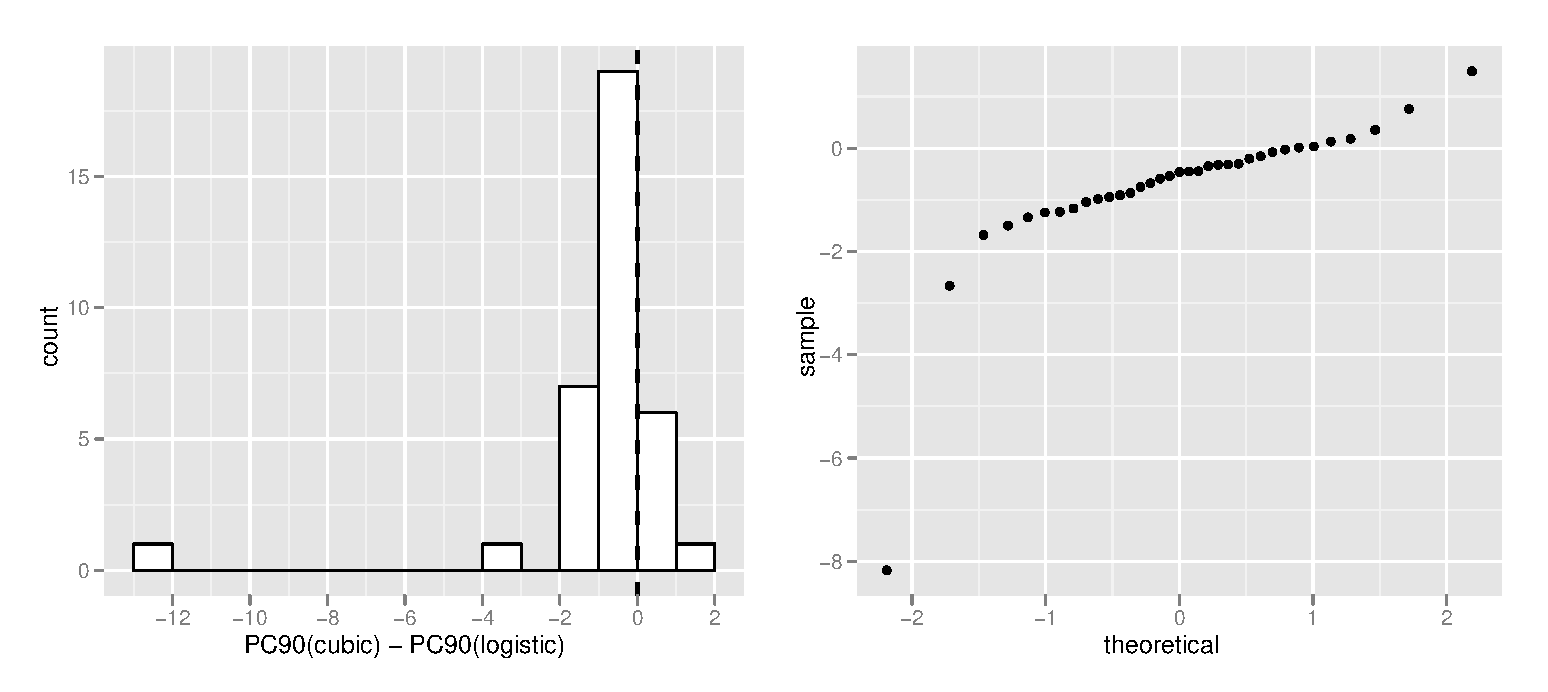
\includegraphics[width=6.5in]{cub-log.eps} 
\caption{Distribution of the difference between PC90 estimated by the cubic and logistic methods}
\label{cub-log}
\end{figure}
Apart from one outlying datum it can be seen that the differences are approximately normally distributed. The outlying value corresponds to subject 183, which we can see in Figure \ref{pc90-bad} gives a very different estimate by the two methods due to the parasite count being fairly constant around the PC90 level. If we perform a paired $t$ test between the PC90 estimates by the cubic and logistic methods, excluding subject 183, we find good evidence to reject the hypothesis that the two methods result in the same PC90 estimate ($P<0.005$). On average the logistic method gives PC90 32 minutes longer than the cubic method with a 95\% confidence interval of (13, 51) minutes, bearing in mind this is only based on a comparison of the subset of 35 subjects for which a logistic fit was possible out of the total of 43.

The distribution of the difference between PC90 estimated by the cubic and logistic methods is shown in Figure \ref{cub-loglin}.
\begin{figure}[h]
\includegraphics[width=6.5in]{cub-loglin.eps} 
\caption{Distribution of the difference between PC90 estimated by the cubic and log-linear interpolation methods}
\label{cub-loglin}
\end{figure}
Again the distribution is approximately normally distributed apart from a single outlying value corresponding to subject 509. We can see in Figure \ref{pc90-bad} that again this corresponds to estimates made in a region where the parasite count is flat. A paired $t$ test excluding subject 509 gives no evidence to reject the hypothesis that the cubic and log-linear interpolation methods give the same PC90 estimates.

The distribution of the difference between PC90 estimated by the logistic and log-linear interpolation methods is shown in Figure \ref{cub-loglin}.
\begin{figure}[h]
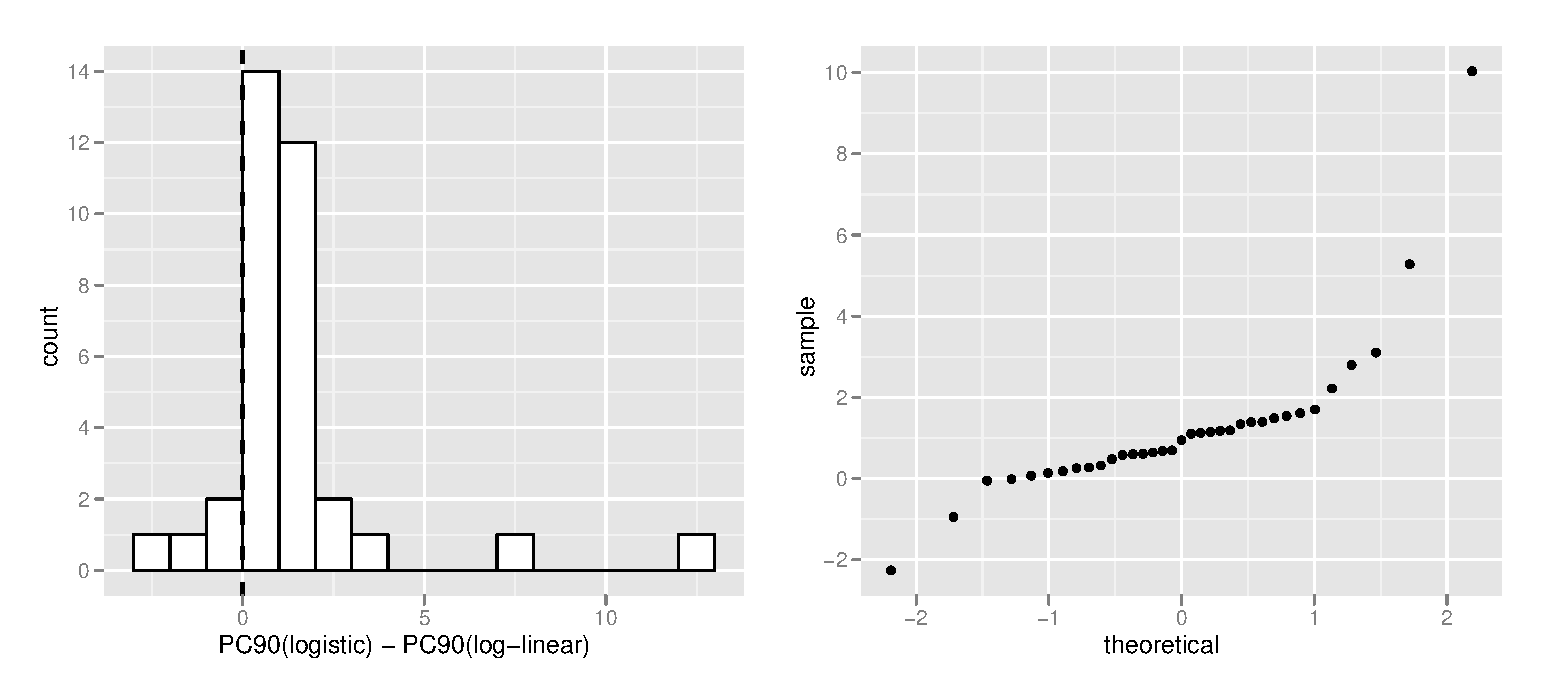
\includegraphics[width=6.5in]{log-loglin.eps} 
\caption{Distribution of the difference between PC90 estimated by the logistic and log-linear interpolation methods}
\label{log-loglin}
\end{figure}
The two outlying values correspond to subjects 183 and 509 again. A paired $t$ test excluding these values gives good evidence to reject the hypothesis that the logistic and log-linear methods produce the same PC90 estimates ($P<0.0005$). On average the logistic method produces PC90 estimates 49 minutes longer than the log-linear interpolation method with a 95\% confidence interval of (25, 73) minutes.

If we perform 4-way ANOVA on the 121 PC90 estimates (3 estimates for each of 43 subjects, minus 8 where no logistic estimate could be made), classified by estimation method, centre, sex and treatment with all interactions we find no evidence that the variance in PC90 between estimation methods is any larger than the variance between subjects in each centre-sex-treatment stratum. The full results of the relative effects of all factors can be found in the next chapter. At this stage we are just concerned with the effect of choice of PC90 estimation method.

We have deduced from the 4-way ANOVA with interactions that there is no interaction between the method chosen and the other factors that influences the PC90 estimation. The $t$ tests told us the average amount that the methods differ, if at all, and in which direction, but we should check if the difference between the methods is related to the size of the PC90 estimates. The difference in PC90 estimate between the methods is plotted against the mean estimate in Figure \ref{pc90est-cor}.
\begin{figure}[h]
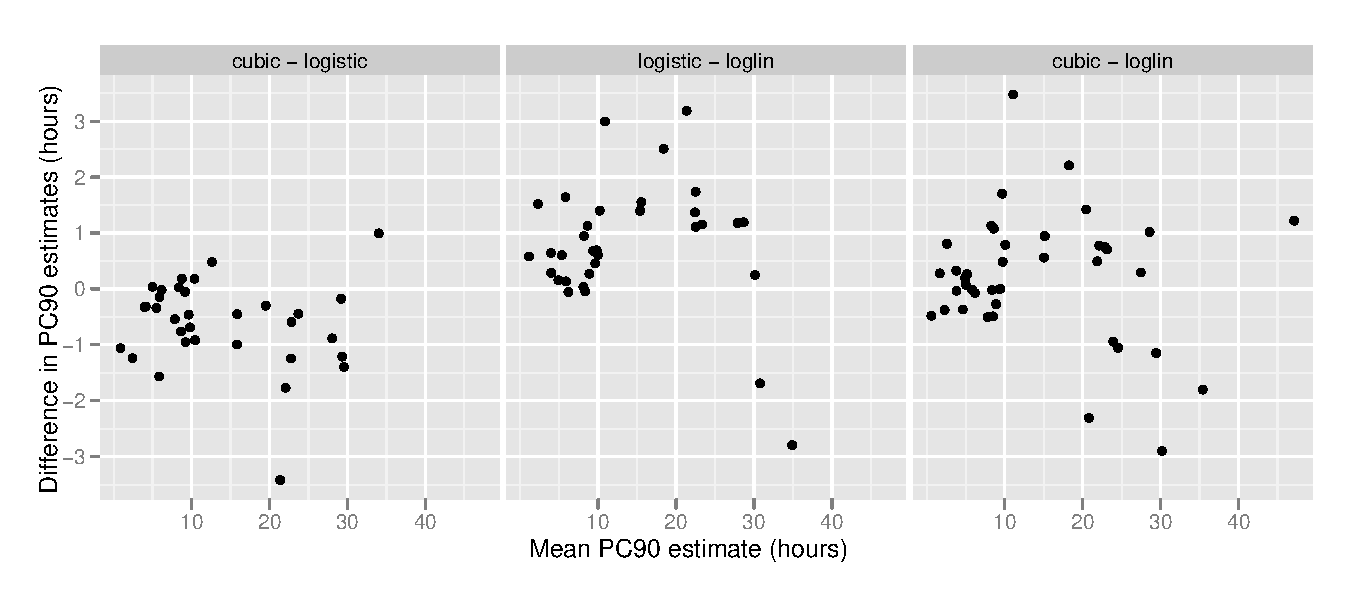
\includegraphics[width=6.5in]{pc90est-cor.eps} 
\caption{Difference in PC90 estimates against mean PC90 estimate}
\label{pc90est-cor}
\end{figure}
There is no obvious correlation and Spearman rank tests do not give any evidence to reject the null hypothesis of 0 correlation. This means that we can expect the methods to give PC90 estimates that differ by the amounts given by the $t$ tests independent of the size of the PC90 estimate.
\clearpage
\section{Key Results}
\chapter{Analysis of Parasite Clearance Times}
\begin{table}[h]
\centering
\caption{Derived PC90 values}\label{pc90}
\begin{tabular}{|cc|c|c|}
\hline
&&\multicolumn{2}{c|}{Treatment}\\
Centre&Sex&A&B\\\hline
\multirow{2}{*}{001}&M&$\begin{array}{c}3.8,\ 27.9,\ 34.3,\  9.8,\\5.0,\  0.8,\ 28.9,\  4.7\end{array}$&$\begin{array}{c}9.5,\  5.3,\  7.7,\\23.5,\  9.4,\  8.1\end{array}$\\\cline{2-4}
&F&$\begin{array}{c}21.1,\ 23.2,\\22.5,\ 47.2\end{array}$&$\begin{array}{c}4.2,\ 8.6 ,\ 9.4,\\0.9,\ 8.6,\ 12.9\end{array}$\\\hline
\multirow{2}{*}{002}&M&$\begin{array}{c}4.5,\ 2.1,\\20.6,\ 29.1\end{array}$&$\begin{array}{c}19.3,\ 10.0,\\15.6,\ 8.9\end{array}$\\\cline{2-4}
&F&$\begin{array}{c}20.1,\ 2.2,\ 24.0,\ 28.7,\\5.0,\ 22.2,\ 23.7\end{array}$&$\begin{array}{c}15.4,\  8.4,\\5.9,\ 6.3\end{array}$\\\hline
\end{tabular}
\end{table}
\subsection{PC90 ANOVA} 
3-way ANOVA with interactions was performed on the PC90 data over centre, sex and treatment. The results are shown in Table \ref{anova}. It can be seen that the only significant effect on PC90 is the treatment used (\texttt{trt}), with perhaps some effect of the interaction between sex and treatment. This is a result we might expect. If we fit a model with treatment as the only factor we find that treatment B reduces the PC90 time compared to treatment A by 8.0 hours with a 95\% confidence interval of (1.9, 14.1) hours.
\begin{table}[h]
\centering
\caption{3-way ANOVA with interactions for PC90}\label{anova}
\begin{boxedverbatim}
Response: PC90
                                         Df Sum Sq Mean Sq F value  Pr(>F)  
factor(SEX)                               1   49.4    49.4  0.5218 0.47488  
factor(CENTREID)                          1    0.1     0.1  0.0008 0.97816  
factor(trt)                               1  697.5   697.5  7.3708 0.01022 *
factor(SEX):factor(CENTREID)              1   57.4    57.4  0.6062 0.44146  
factor(SEX):factor(trt)                   1  389.4   389.4  4.1151 0.05016 .
factor(CENTREID):factor(trt)              1  143.4   143.4  1.5150 0.22658  
factor(SEX):factor(CENTREID):factor(trt)  1   49.3    49.3  0.5214 0.47505  
Residuals                                35 3312.0    94.6
\end{boxedverbatim}
\end{table}

Diagnostic plots of the residuals of the ANOVA model are shown in Figure \ref{resid}. There does not seem to be any significant departure from normality in the distribution of residuals which suggests that we may not need a transformation for modelling the PC90 data. However, there is perhaps some evidence of heteroskedasticity in that the variance of the residuals appears to increase with increasing fitted PC90 value, hence we may need a variance-stabalising transformation.
\begin{sidewaysfigure}[p]
\centering
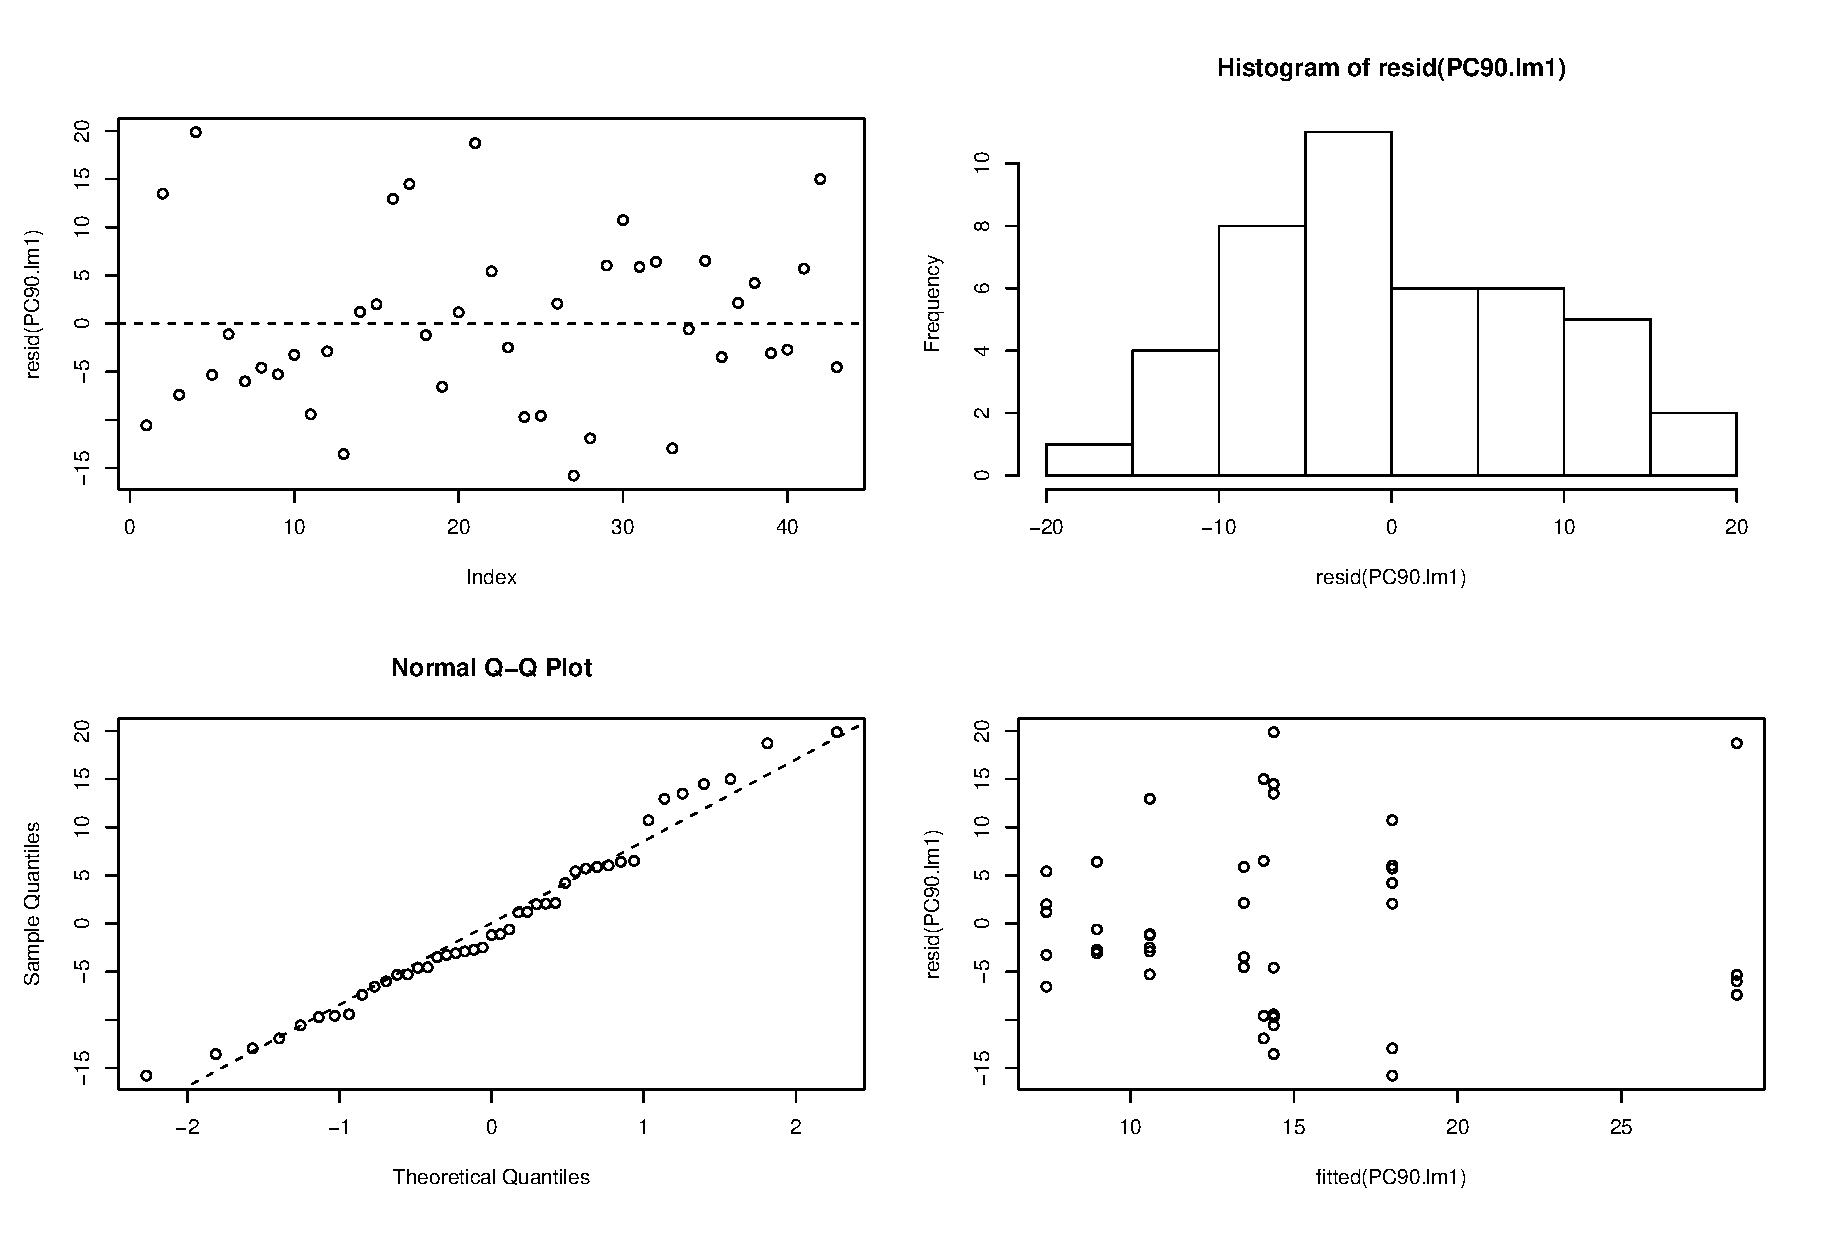
\includegraphics[scale=0.8]{PC90diag.eps}
\caption{Residuals for ANOVA on PC90}\label{resid}
\end{sidewaysfigure}

\chapter{Alternative Measures of Clearance Time}\label{ch:alternative}

\section{Alternative endpoints}
\subsection{PC50}
PC50 was estimated by log-linear interpolation. The PC50 clearance times thus obtained are plotted in Figure \ref{pc50anova} by experimental factors with sub-plots to look for interactions.
\begin{figure}[p]
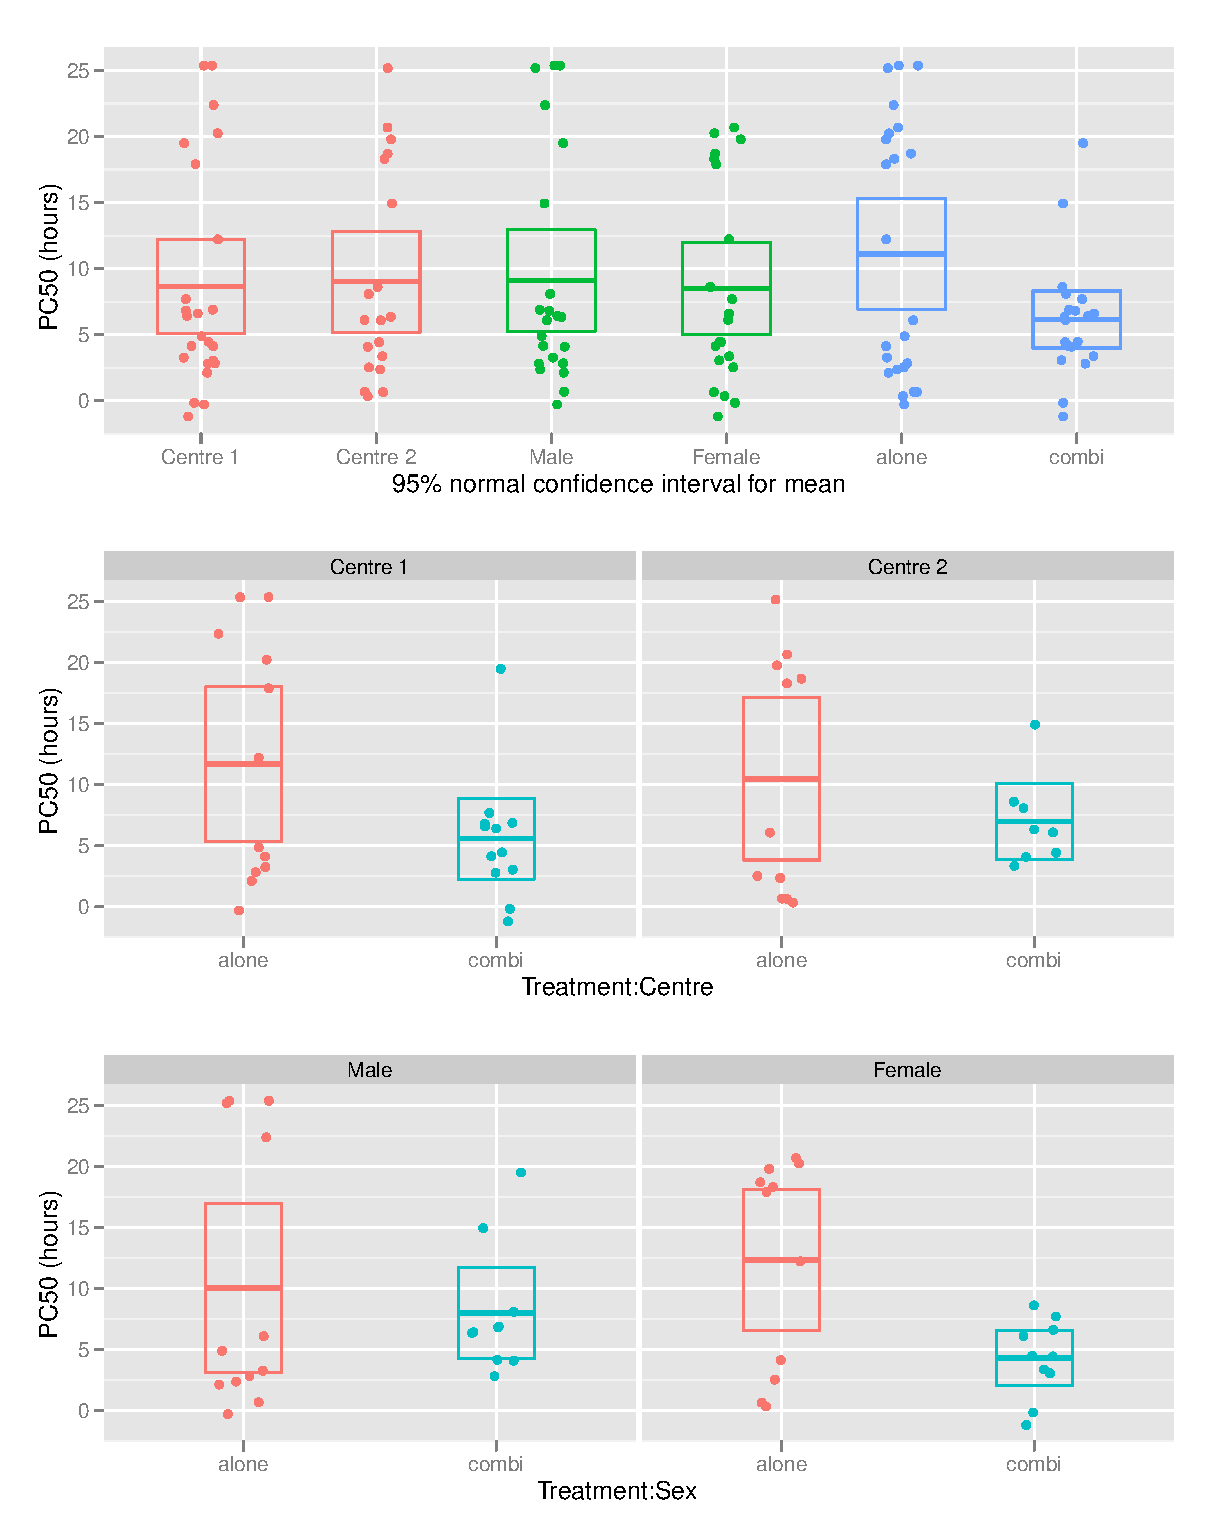
\includegraphics[width=150mm]{pc50anova.eps} 
\caption{Comparison of PC50 main effects and interactions with $t$ distribution 95\% confidence intervals for the means}
\label{pc50anova}
\end{figure}
A similar pattern can be seen as for PC90 (Figures \ref{pc90boxes} and \ref{pc90interaction} on pages \pageref{pc90boxes} and \pageref{pc90interaction}). The same key features are present namely
\begin{itemize}
\item No difference between centres.
\item A reduction in clearance time with the combined treatment, but only for female subjects.
\item A greater variance for subjects on the single (``alone'') treatment.
\end{itemize}

The same procedure of inspecting the distribution of standardized residuals was followed for choosing an appropriate ANOVA model for the data. As with PC90 it was found that the most suitable model for the PC50 clearance time was a 2-way ANOVA model by sex and treatment with a square-root transformation of the dependent variable, fitted by weighted least-squares, using the variances of the two treatment groups as the weighting. The results are shown in Table \ref{aov50}.
%> summary(PC50.loglin2rwt.aov)
%              Df Sum Sq Mean Sq F value  Pr(>F)  
%Sex            1  1.104   1.104  1.1652 0.28702  
%Treatment      1  2.089   2.089  2.2055 0.14556  
%Sex:Treatment  1  3.010   3.010  3.1771 0.08246 .
%Residuals     39 36.949   0.947
\begin{table}[h]
\centering
\caption{ANOVA table for PC50 model}\label{aov50}
\begin{tabular}{l|rrrrrl}
Source&Sum Sq.&df&Mean Sq.&$F$&P($>F$)\\
\hline
$Sex$				& 1.10 & 1 & 1.10 & 1.17 & 0.287 & \\
$Treatment$			& 2.09   & 1 & 2.09   & 2.21   & 0.146 & \\
$Sex\times Treatment$	& 3.01   & 1 & 3.01   & 3.18   & 0.082 & \\
$Residuals$			& 36.95 & 39 & 0.947 &&&\\
\hline
Total&43.15&42&&&
\end{tabular}
\end{table}

Although Figure \ref{pc50anova} seems to show a sex-treatment interaction effect on clearance times we do not have evidence at the 5\% level to reject the hypothesis that there is no effect of sex or treatment. This is probably because the difference between clearance times is smaller than for PC90 and we don't have enough data to detect this difference at the 5\% level.

The mean PC50 clearance times and confidence intervals are shown in Table \ref{inference50}.
\begin{table}[h]
\centering
\caption{Mean PC50 clearance times by sex and treatment}\label{inference50}
\begin{tabular}{|l|c|c|}
\hline
&Clearance time PC50&95\% conf. int.\\
Factor levels&(hrs:mins)&(hrs:mins)\\
\hline
Male, single treatment 		& 6:47 & (2:37, 12:54) \\
Female, single treatment		& 10:02 & (4:34,  17:37) \\
Male, combined treatment	& 7:22 & (3:50, 12:03) \\
Female, combined treatment	& 2:54 & (0:54, 6:03) \\
\hline
\end{tabular}
\end{table}

For female subjects the mean decrease in PC50 in the combined treatment group over the single treatment group is 7.1 hours with a 95\% confidence interval of (0.7, 9.9) hours.

\subsection{PC99}
%The log-linear interpolated PC99 values are plotted in Figure \ref{pc99anova}.
%\begin{figure}[p]
%\includegraphics[width=150mm]{pc99anova.eps} 
%\caption{Comparison of PC99 main effects and interactions with $t$ distribution 95\% confidence intervals for the means}
%\label{pc99anova}
%\end{figure}
For 3 subjects the parasite count did not reach the PC99 level by the end of the study. Rather than simply omit these subjects and thereby bias the comparison - as these 3 subjects are ones with long clearance times on the single treatment - we can make estimates of the possible range of PC99 for these subjects had data been taken for a longer time period. In order to do this we make a linear extrapolation to the PC99 level as shown in Figure \ref{pc99extrap} for subjects 285 and 98.
\begin{figure}[h]
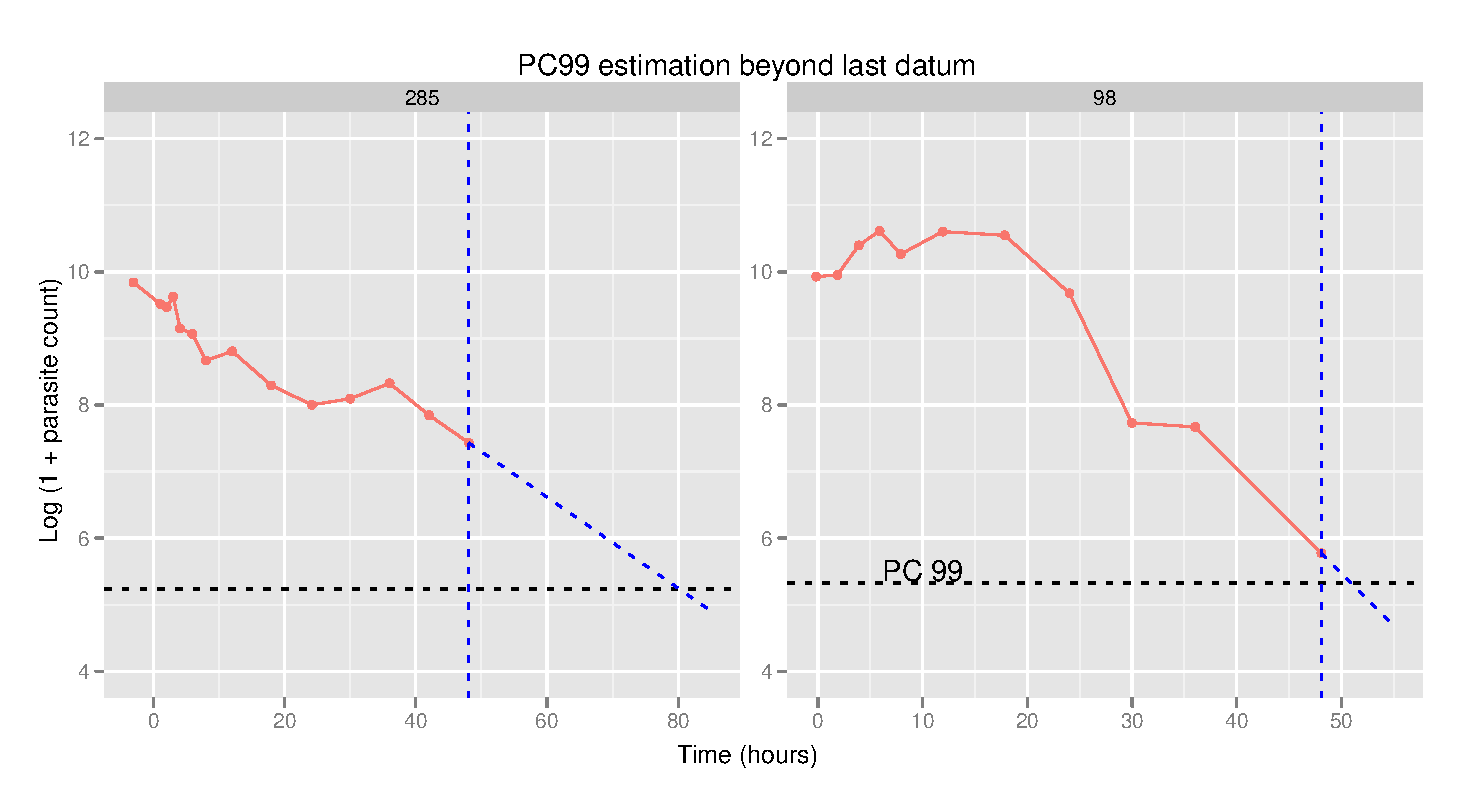
\includegraphics[width=150mm]{pc99extrap.eps} 
\caption{Bounds for PC99 estimates between immediate cut-off (lower estimate) and linear extrapolation (upper estimate)}
\label{pc99extrap}
\end{figure}
We define an upper estimate for PC99 as that predicted by linear extrapolation and a lower estimate simply assumes that the parasite count dropped below PC99 immediately after the last reading.

For subject 477 the parasite count drops below PC99 but then rises again as shown in Figure \ref{477}.
\begin{figure}[h]
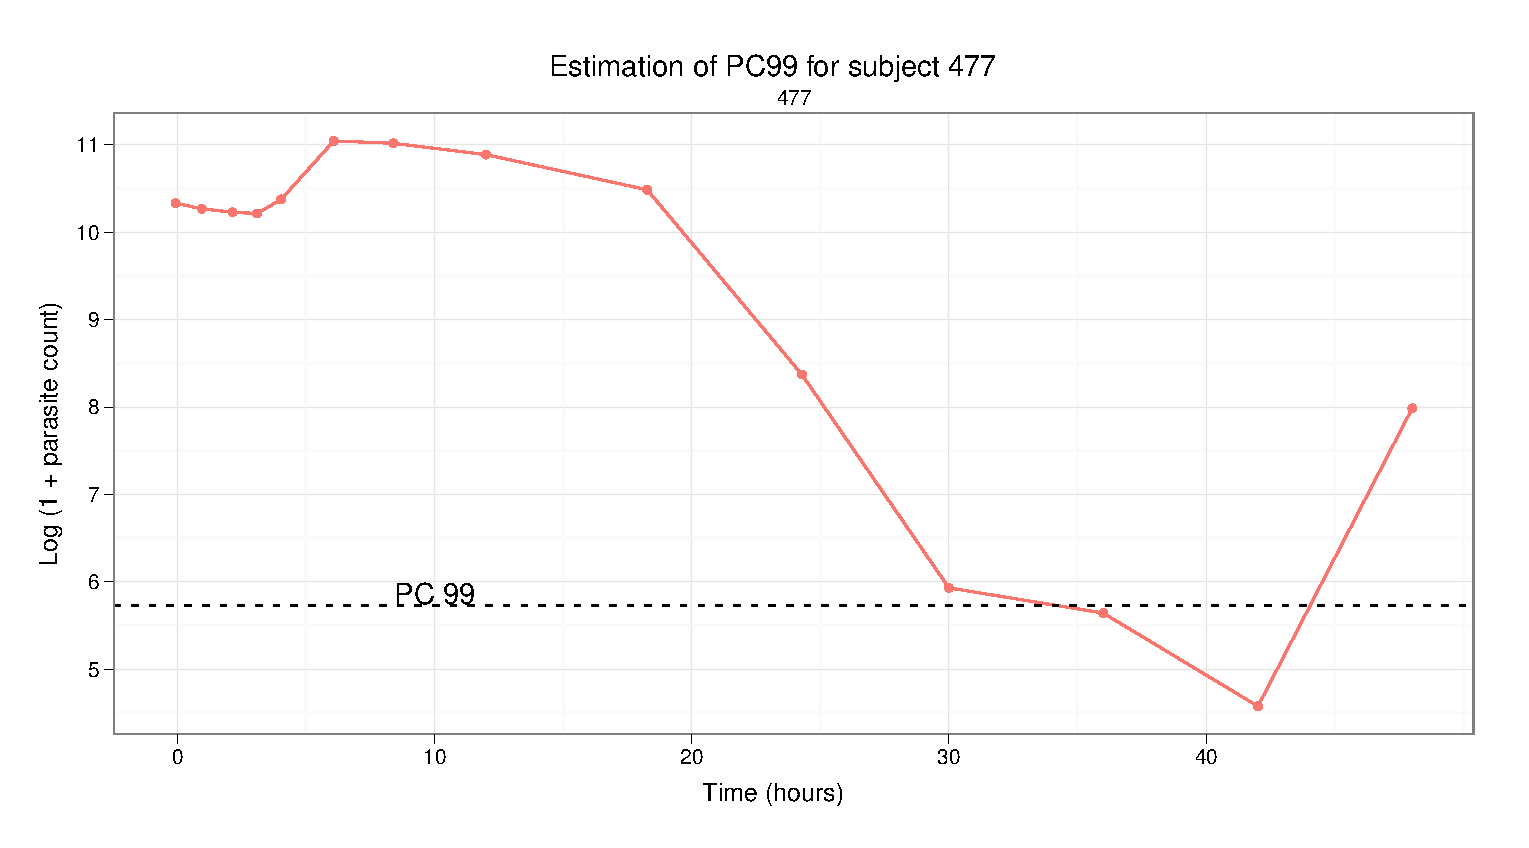
\includegraphics[width=150mm]{477.eps} 
\caption{PC99 estimation for subject 477}
\label{477}
\end{figure}
In this case we can take the lower bound for the estimate as the first time the PC99 is reached, thereby assuming that the last datum is a false reading. It is not clear what to use as the upper estimate, but a starting point is to set it equal to the largest PC99 value observed.

%Once again there is no discernible effect of centre or sex alone on the clearance times. However, now the improvement of the combined treatment over the single treatment seems more symmetrical between sexes.
Results of 2-way ANOVA by sex and treatment on the square-root transformed clearance times fitted by treatment-weighted least-squares are shown in Table \ref{aov99}, using the lower and upper estimates for PC99 for the 2 subjects where PC99 was not reached and subject 477 where the parasite count rose again after PC99.
%              Df Sum Sq Mean Sq F value    Pr(>F)    
%Sex            1  0.926   0.926  0.8609 0.3591839    
%Treatment      1 15.809  15.809 14.7031 0.0004477 ***
%Sex:Treatment  1  2.228   2.228  2.0720 0.1580030    
%Residuals     39 41.934   1.075            
\begin{table}[h]
\centering
\caption{ANOVA tables for PC99 model using lower and upper estimates for missing data}\label{aov99}
Lower estimates
\begin{tabular}{l|rrrrrl}
Source&Sum Sq.&df&Mean Sq.&$F$&P($>F$)\\
\hline
$Sex$				& 0.926 & 1 & 0.926 & 0.861 & 0.359 & \\
$Treatment$			& 15.81   & 1 & 15.81   & 14.70   & 0.0004 &*** \\
$Sex\times Treatment$	& 2.23   & 1 & 2.23   & 2.07   & 0.158 & \\
$Residuals$			& 41.93 & 39 & 1.08 &&&\\
\hline
Total&60.90&42&&&
\end{tabular}\\[1ex]
Upper estimates
%              Df Sum Sq Mean Sq F value    Pr(>F)    
%Sex            1  0.216   0.216  0.1464 0.7040962    
%Treatment      1 22.011  22.011 14.8867 0.0004173 ***
%Sex:Treatment  1  4.736   4.736  3.2028 0.0812809 .  
%Residuals     39 57.665   1.479
\begin{tabular}{l|rrrrrl}
Source&Sum Sq.&df&Mean Sq.&$F$&P($>F$)\\
\hline
$Sex$				& 0.216 & 1 & 0.216 & 0.146 & 0.704 & \\
$Treatment$			& 22.01   & 1 & 22.01   & 14.89   & 0.0004 &*** \\
$Sex\times Treatment$	& 4.74   & 1 & 4.74   & 3.20   & 0.081 & \\
$Residuals$			& 57.67 & 39 & 1.48 &&&\\
\hline
Total&60.90&42&&&
\end{tabular}\\
\hspace{20em}***$<0.0005$
\end{table}

It can be seen that there is good evidence to reject the hypothesis that treatment has no effect on PC99 clearance time, but no evidence to reject the hypothesis that sex has no effect. Raising the upper estimate of subject 477 to over 100 does not alter the outcome of the hypothesis tests. Since subject 477 is male and the other two subjects for whom an extrapolated PC99 estimates were made are female, the ANOVA was repeated with the high and low estimates set opposite between sexes. This did not alter the outcome of the hypothesis tests.

If we average over both lower and upper estimates for the missing data, this gives a reduction in PC99 for subjects on the combined treatment of 12.1 hours with a 95\% confidence interval of (7.5, 16.9) hours.
%Therefore, we can exclude sex as a factor and refit a 1-way ANOVA model by treatment alone, giving the results shown in Table \ref{aov99r}.
%%            Df Sum Sq Mean Sq F value  Pr(>F)   
%%Treatment    1  9.396   9.396  9.3959 0.00399 **
%%Residuals   38 38.000   1.000   
%\begin{table}[h]
%\centering
%\caption{1-way ANOVA table for PC99 model}\label{aov99r}
%\begin{tabular}{l|rrrrrl}
%Source&Sum Sq.&df&Mean Sq.&$F$&P($>F$)\\
%\hline
%$Treatment$			& 9.40   & 1 & 9.40   & 9.40   & 0.004 &** \\
%$Residuals$			& 38.0 & 38 & 1.00 &&&\\
%\hline
%Total&47.40&39&&&
%\end{tabular}\\
%**$<0.005$
%\end{table}

%The mean PC99 clearance time for patients on the single treatment is 21:07 (hrs:mins) with a 95\% confidence interval of (16:12, 26:41); for the combined treatment it is 12:33 (9:53, 15:32). This gives a mean decrease in PC99 for subjects on the combined treatment over the single treatment of 9.3 hours with a 95\% confidence interval of (3.7, 15.0) hours.

%\subsubsection{Survival analysis}
%An alternative method to handle the effectively \emph{right-censored} PC99 times is to use survival analysis techniques. If we define an ``event'' as the parasite count being reduced by 99\% then we have a set of ``survival'' times up to the occurrence of our event of interest with 3 right-censored times at 48 hours.

\subsection{Parasite reduction ratios}
Another endpoint used in studies of the efficacy of antimalarial drugs is the \emph{Parasite Reduction Ratio}, which is the ratio of the pre-dose parasite count to the count at a specific time from the time of first dose. 48 hours is often chosen as a time to calculate this ratio (PRR$_{48}$) as this represents the reduction in parasites over a single life-cycle of the parasites \cite{white}. ``PRR$_{24}$'', The reduction over 24 hours is also used \cite{newton}.

PRR$_{48}$ measurements are not available for our data as the parasite count is 0 by 48 hours for all but 6 subjects. After 24 hours there are only 25 of the 43 subjects with non-zero parasite counts. Even after 12 hours there are only 37 of the 43 subjects with a non-zero parasite counts. Consequently, it was decided that analysis of parasite reduction ratios was not suitable for this data.

An alternative, but similar approach is to look at the ratio of the count at a specific time to the pre-dose count, which is effectively 1/PRR. This has already been looked at in section \ref{sec:develt} and is studied further in the next section on functional data analysis.
%so we can look at PRR12 and have reasonable numbers in groups to make comparisons between treatments. The log parasite reduction ratio after 12 hours is shown in Figure \ref{prr12}
%\begin{figure}
%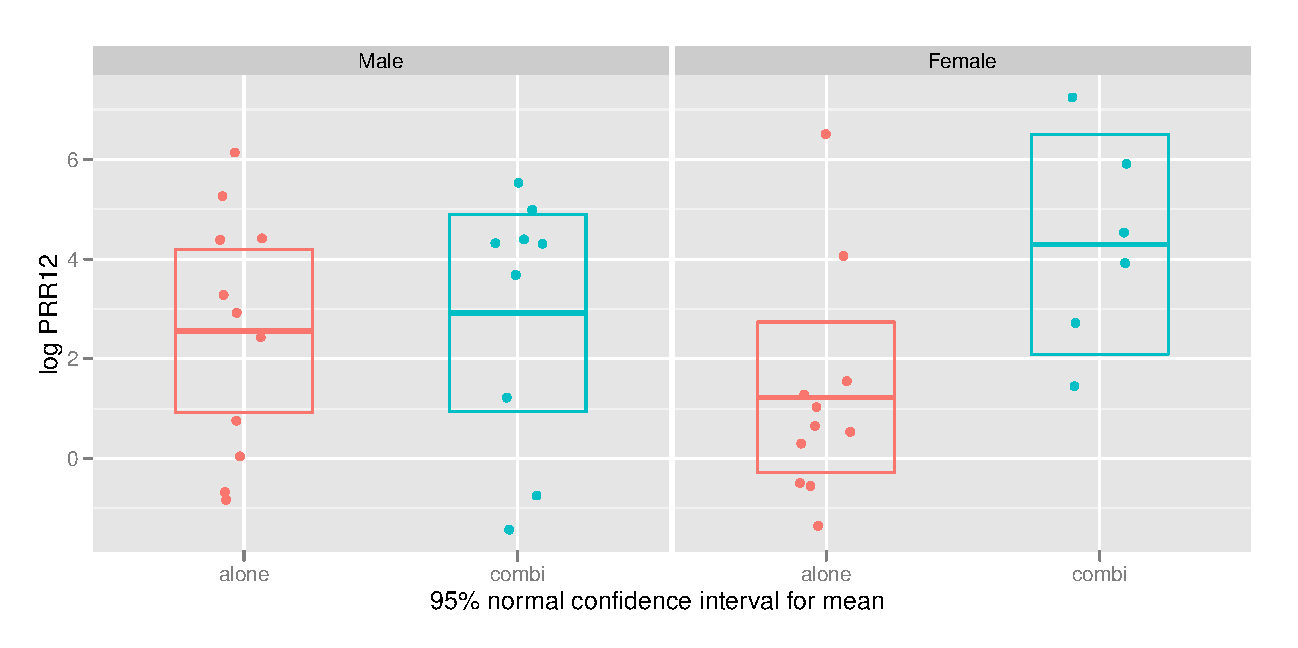
\includegraphics[width=150mm]{prr12.eps} 
%\caption{log PRR12 with 95\% confidence intervals for the means}
%\label{prr12}
%\end{figure}

%A similar pattern as with the PC90 and PC50 endpoints can be seen in that the treatment only seems to be effective among female patients in increasing PRR. It was found that a logarithmic transformation was appropriate for 2-way ANOVA modelling of the PRR12 data giving the results shown in Table \ref{aovprr12}.
%%              Df  Sum Sq Mean Sq F value  Pr(>F)  
%%Sex            1   1.524   1.524  0.2725 0.60512  
%%Treatment      1  21.265  21.265  3.8024 0.05972 .
%%Sex:Treatment  1  15.951  15.951  2.8521 0.10069  
%%Residuals     33 184.557   5.593          
%\begin{table}[h]
%\centering
%\caption{ANOVA table for PC99 model}\label{aovprr12}
%\begin{tabular}{l|rrrrrl}
%Source&Sum Sq.&df&Mean Sq.&$F$&P($>F$)\\
%\hline
%$Sex$				& 1.52 & 1 & 1.52 & 0.273 & 0.605 & \\
%$Treatment$			& 21.27   & 1 & 21.27   & 3.80 & 0.060 & \\
%$Sex\times Treatment$	& 15.95   & 1 & 15.95   & 2.85   & 0.101 & \\
%$Residuals$			& 184.56 & 33 & 5.59 &&&\\
%\hline
%Total&223.30&36&&&
%\end{tabular}
%\end{table}

%It can be seen that there is some evidence between the 5 and 10\% level to reject the hypothesis that the treatment has no effect on the parasite reduction ratio after 12 hours. It may be that we don't have enough data to detect the treatment effect observed in Figure \ref{prr12}. The model gives a mean increase in PRR12 for subjects on the combined treatment over those on the single treatment of 25.5 with a 95\% confidence interval of (-0.4, 159.8).

%\subsection{Logistic model of those cured after 24 hours?}

\section{Functional data analysis}
\subsection{Overview of functional data analysis}
Functional data analysis (FDA) is a relatively new technique whereby data is analysed in terms of smooth functions. An example is longitudinal data such as the growth of children or the weather over a year \cite{ramsay}. With such data we describe the response with a smooth function and then look at the ways the characteristics of the function change between cases. For example, this type of analysis can make use of derivatives of the functions to look for patterns in rates of change. Functional data analysis is somewhat analogous to multivariate data analysis, looking at multiple responses and characteristic combinations of responses between cases.

The parasite count data in this study is a good candidate for functional data analysis in that the response for each replicate of experimental factors centre, sex and treatment can be described as a smooth function of parasite count with time. We already used cubic and logistic functions in order to extract a single response variable, the PC90 clearance time, but now we can go on to explore the nature of a functional response.

Many familiar statistical summaries and techniques have functional equivalents. Means and standard deviations can be expressed as mean functions and standard deviation functions for example. Regression and ANOVA can be performed with functional dependent and independent variables yielding residual, $F$ statistic and coefficient functions.

\subsection{Basis functions}
The first step in FDA is to identify an appropriate smoothing function for our data known as a \emph{basis function}. For periodic data fourier functions are normally used, for non-periodic data the most commonly used basis functions are cubic splines \cite{fdaweb}. Fitting a cubic spline requires choice of \emph{breakpoints} between which we fit cubic polynomials. The simplest choice of breakpoints with longitudinal data is to choose the times at which the data were taken. We also specify a smoothness parameter that limits the size of higher derivatives and hence the sharpness of the curve.

\subsubsection*{Fitting a basis function to the parasite count data}
We want to compare the development of parasite count with time between subjects using a scale that is independent of the absolute count. Hence we will use the fraction of the pre-dose parasite count. We determined that a logarithmic transform of the count is appropriate for this data and hence we will use as our time-dependent variable $y(t)$
$$y(t)=\log (1+P(t))-\log(1+P_{0})$$
which is the logarithm of the ratio of the parasite count at time $t$, $P(t)$, to the pre-dose parasite count $P_{0}$. 1 is added to both so that the logarithm of 0 count is 0.

Ramsay \textit{et al.} have written a \emph{R} package, \texttt{fda} for functional data analysis \cite{fdaR, fdaRbook}. The functions in this package were used to fit cubic splines to the data. The level of smoothing is determined by penalising derivatives of the spline function. It was found that penalising the 2nd derivative (the rate of change of slope) by a factor of 10 gave reasonable smoothing such that the fitted curves were insensitive to small-scale (perhaps random-error scale) variation but described the overall trend of the parasite count well. The resulting curves for the 43 subjects are shown in Figure \ref{cubicspline}.
\begin{figure}[h]
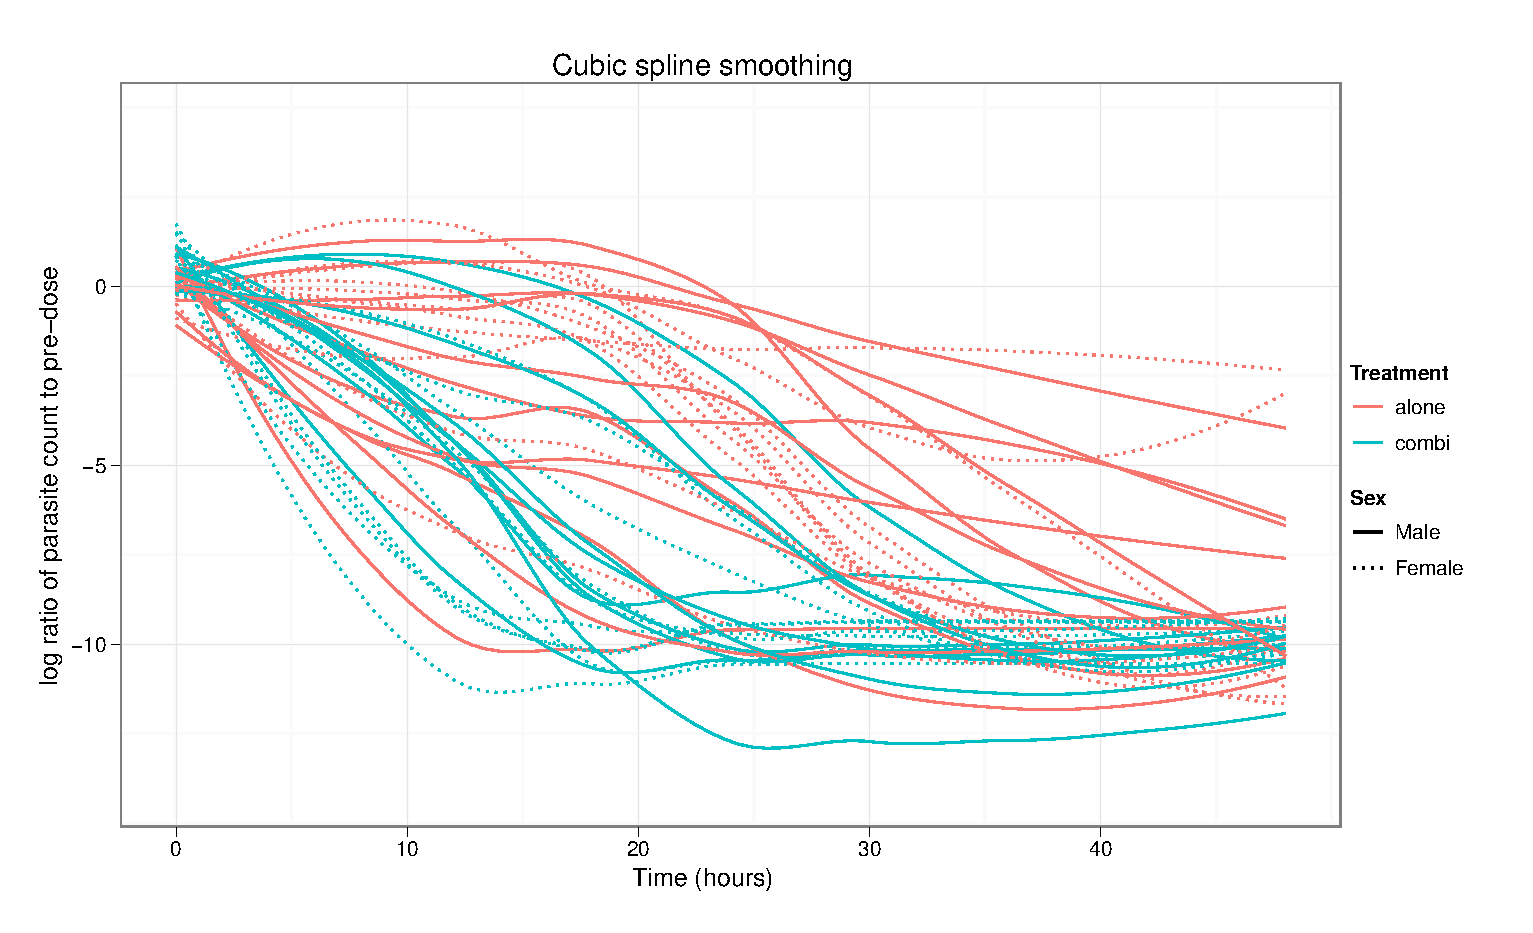
\includegraphics[width=150mm]{cubicspline.eps} 
\caption{Cubic splines fitted to the parasite count, smoothed by penalising the 2nd derivative}
\label{cubicspline}
\end{figure}

\subsection{Functional ANOVA}
Once we have suitably represented our dependent data as a functional response we can perform ANOVA by sex and treatment in an analogous way to the previous analysis (it is assumed that centre has no effect over the whole time period). The model now becomes
\begin{equation}
y_{jkl}(t)=\mu(t)+S_{j}(t)+T_{k}(t)+(ST)_{jk}(t)+\epsilon_{jkl}(t)\quad\quad\epsilon_{jkl}(t)\sim N(0, \sigma^{2}(t))\label{aovfda}
\end{equation}
where each part of the model is now a function of time. Hence, we will have 43 residual functions, a mean function for the overall mean with time, $\mu(t)$, a function for the effect of sex, $S(t)$, and for the effect of treatment, $T(t)$.

The standardized residual functions ($e(t)/\hat{\sigma}(t)$) from fitting this model are shown in Figures \ref{fdaresids} and \ref{fdahistqq}. It can be seen that they are approximately normally distributed about 0 indicating that our parameter function estimates will be unbiased.
\begin{figure}[p]
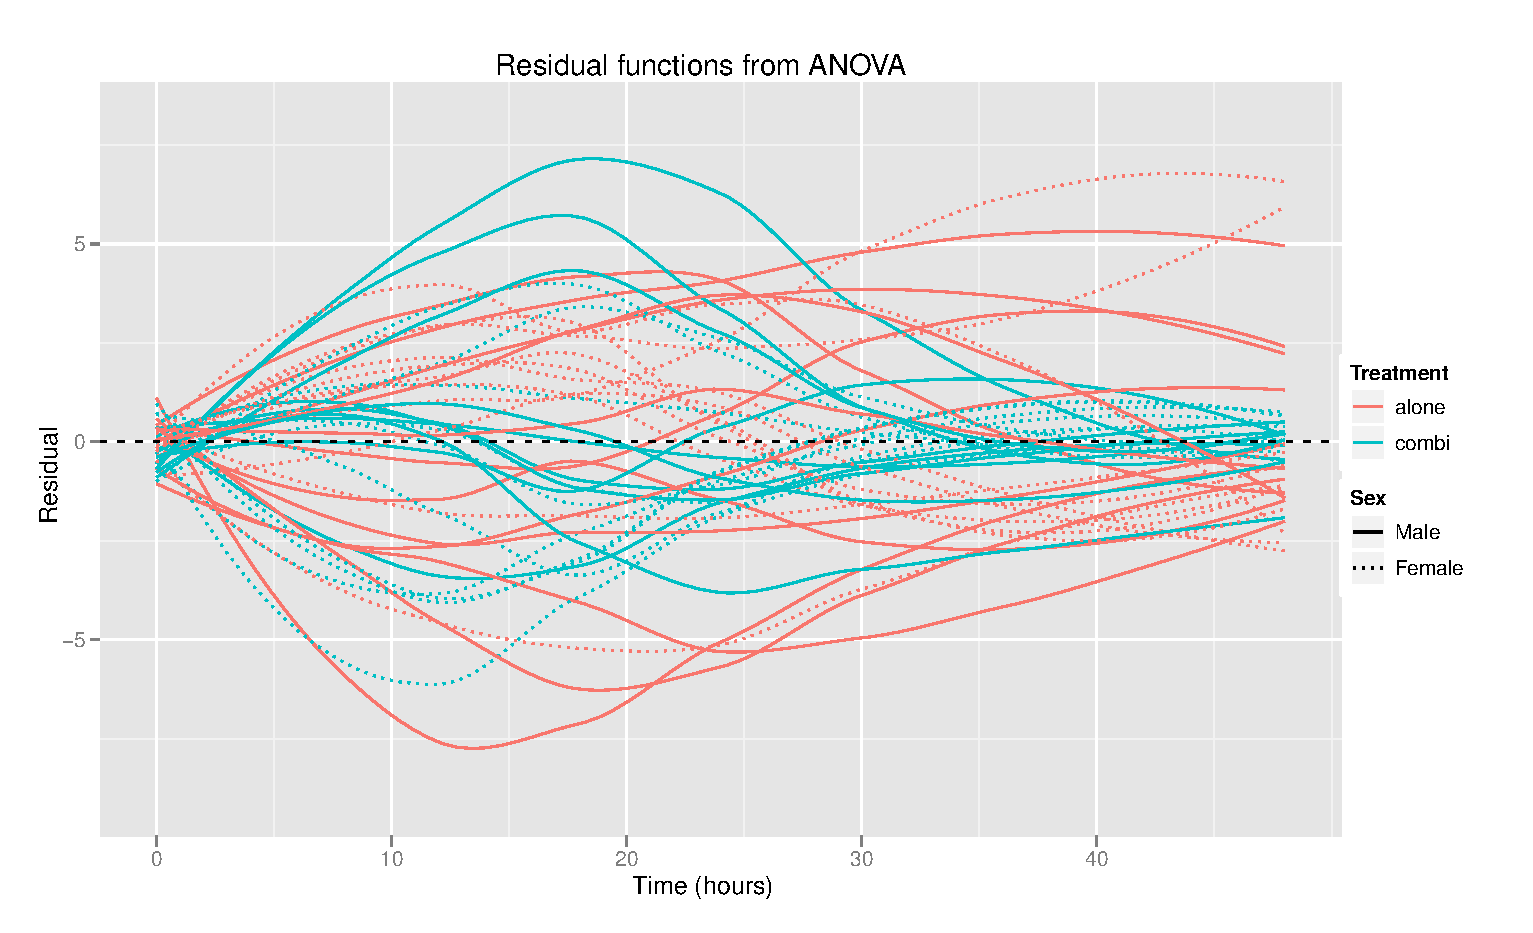
\includegraphics[width=150mm]{fdaresids.eps} 
\caption{Standardized residual functions for 2-way functional ANOVA}
\label{fdaresids}
\end{figure}
\begin{figure}[p]
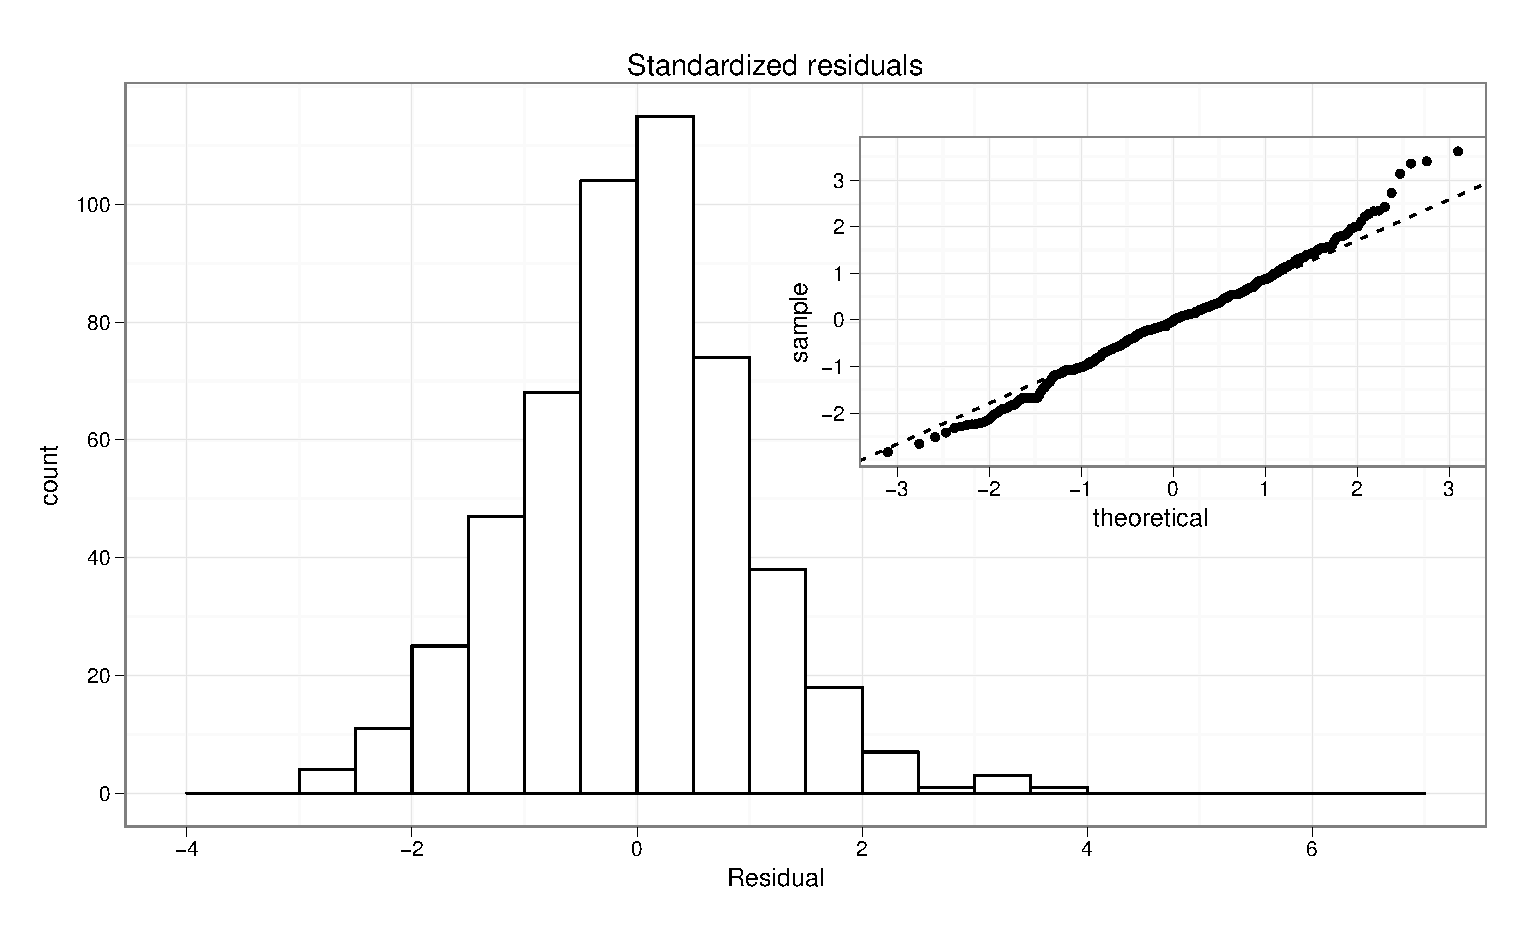
\includegraphics[width=150mm]{fdahistqq.eps} 
\caption{Distribution of standardized residuals for 2-way functional ANOVA}
\label{fdahistqq}
\end{figure}

The \texttt{fda} library provides functions for deriving a permutation $F$ test similar to the methods used in section \ref{section:resampling}. The results of this permutation $F$ test for our 2-way ANOVA are shown in Figure \ref{fdapermF}. The pointwise critical value is relevant if we look at any one time, but for making simultaneous hypothesis tests over all times we should use the maximum critical value shown. It can be seen that the null hypothesis of no difference of sex or treatment groups is not rejected up to 10 hours from first dose, then there is evidence after 10 hours to reject the null hypothesis, with no evidence for rejection after about 30 hours. This can be explained by the parasite count being independent of sex and treatment allocation at the start, with significant differences in the count trajectories developing between the groups as time goes on, with them eventually returning to parity as clearance is finally achieved for all subjects.
\begin{figure}[p]
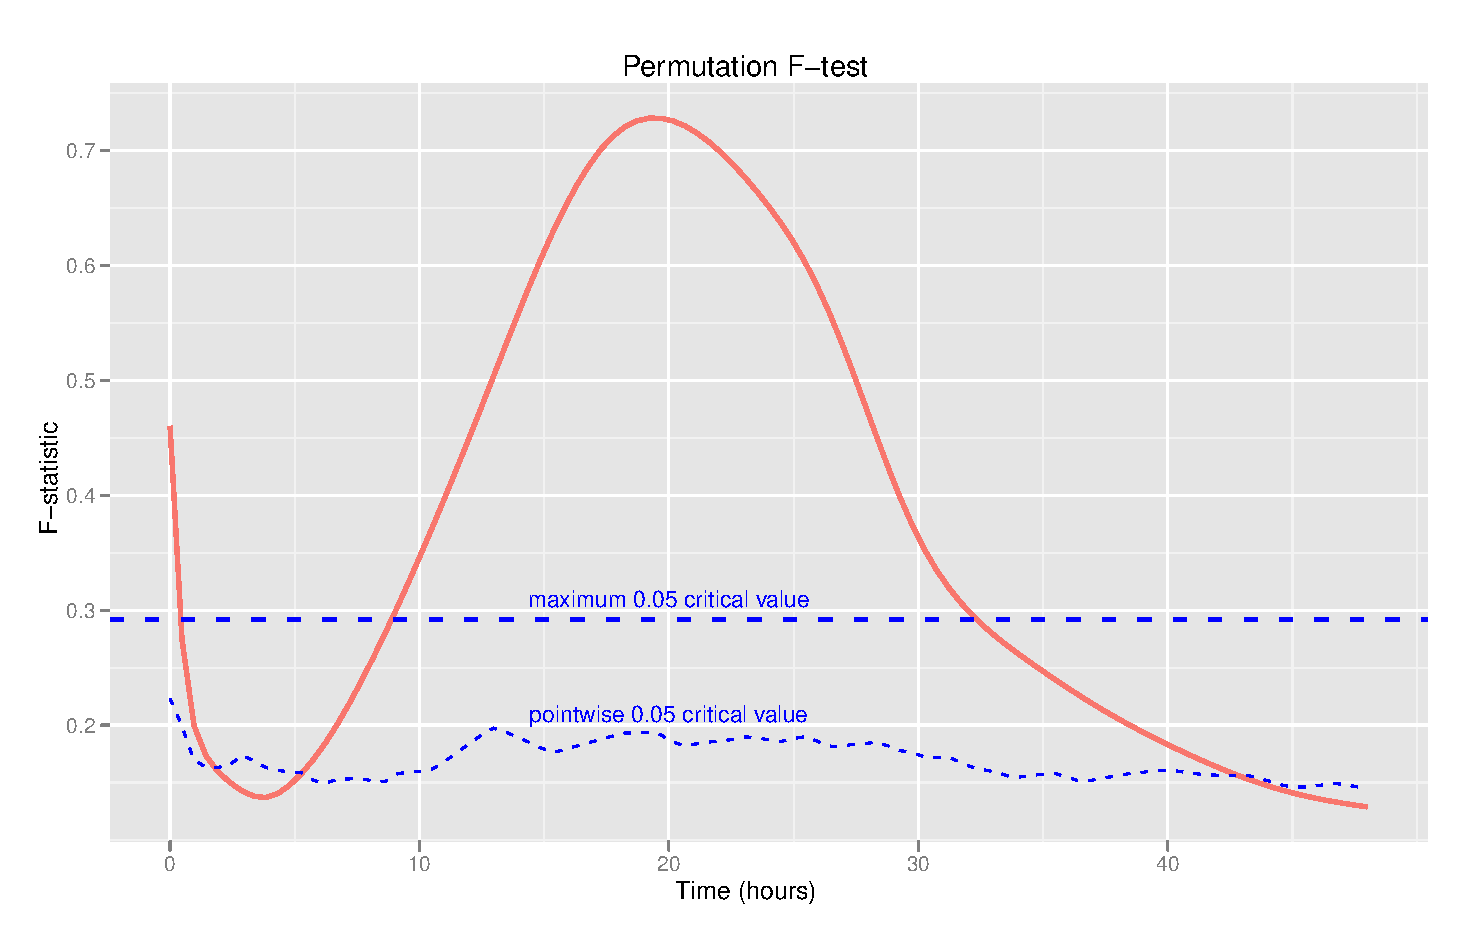
\includegraphics[width=150mm]{fdapermF.eps} 
\caption{$F$ statistic function for 2-way functional ANOVA. The critical value at each time is shown and the critical value for the maximum $F$ statistic over all times.}
\label{fdapermF}
\end{figure}

Figure \ref{fdcoef} shows the fitted coefficient functions.
\begin{figure}[p]
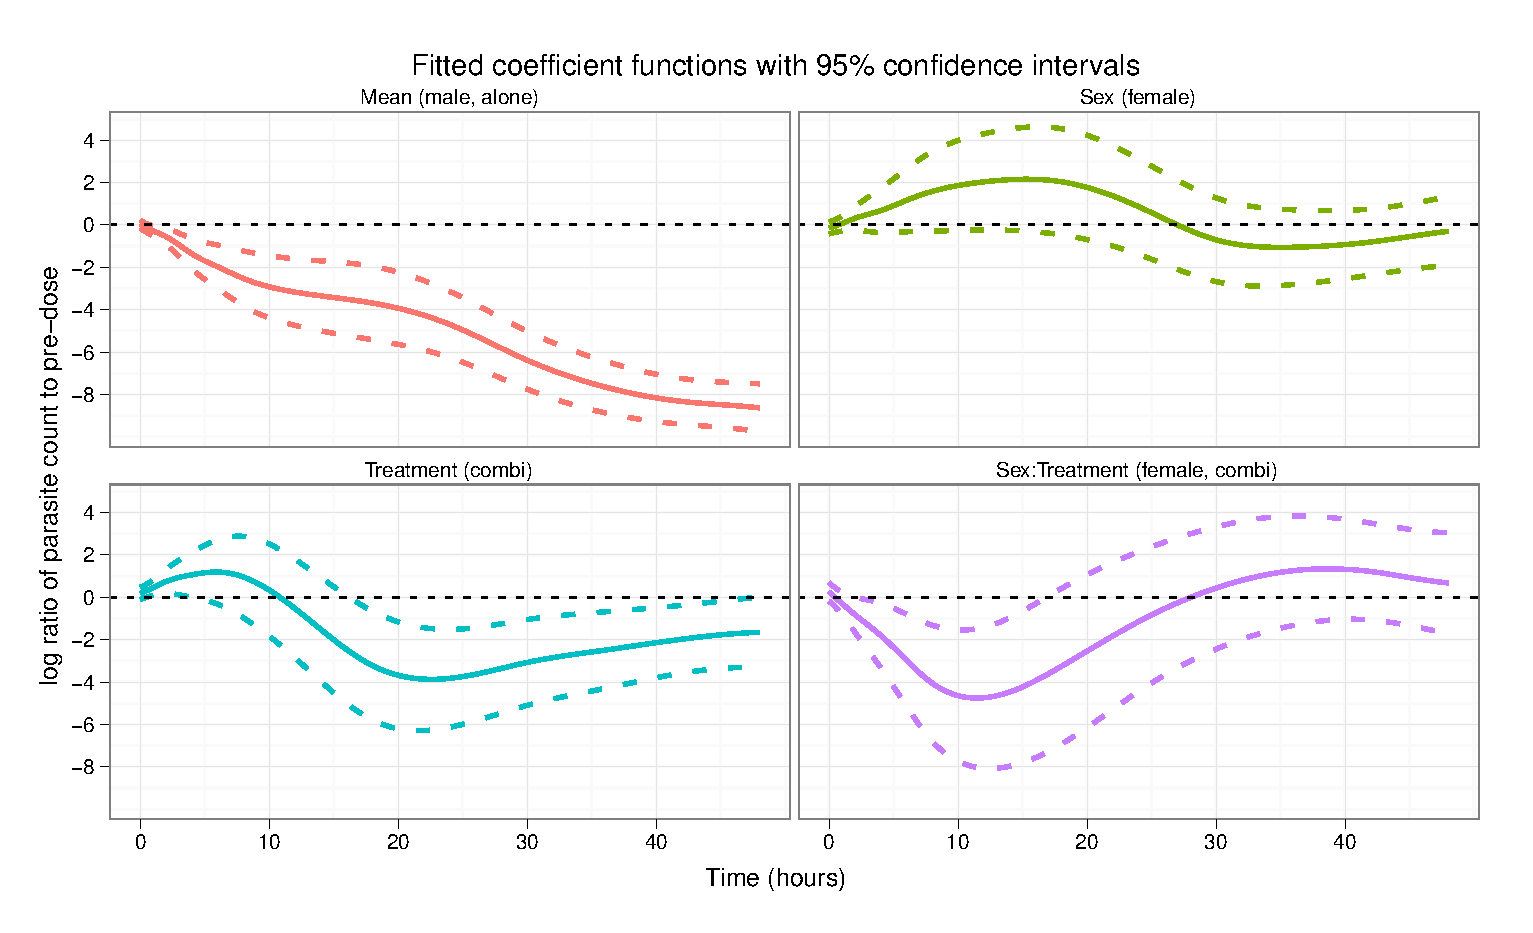
\includegraphics[width=150mm]{fdcoef.eps} 
\caption{Fitted coefficient functions for 2-way ANOVA model \ref{aovfda} (page \pageref{aovfda}). From top-left, to bottom-right, the functions are $\mu(t)$, $S(t)$, $T(t)$, $ST(t)$.}
\label{fdcoef}
\end{figure}
The top-left panel shows the function for the mean $\mu$ corresponding to male subjects on the single treatment with the other panels showing the deviation from this mean due to sex, treatment and the interaction of sex and treatment respectively. We can see that there is evidence at the 5\% level between 10 and 15 hours to reject the hypothesis that there is no interaction between sex and treatment that effects the parasite count. We cannot easily draw conclusions about the sex and treatment main effects separately as there is an interaction effect and hence the main effects act at different levels dependent on each other. However, it seems that after 20 hours the interaction becomes negligible and that the treatment effect acts more evenly on both sexes.

\newpage
The routine for calculating the standard errors and confidence intervals of fitted functions is not yet implemented in the \emph{R} \texttt{fda} library, hence it was necessary to calculate confidence intervals for the fitted response $\hat{y}(t)$ as follows.

The $4\times 1$ vector of predicted mean responses (log count ratios) for each of the four sex-treatment groups with time $t$ is
$$\hat{\mat{y}}(t)=\mat{x}_{0}^{T}\hat{\mat{\beta}}(t)=\{\hat{y}_{MA}(t),\ \hat{y}_{FA}(t),\ \hat{y}_{MC}(t),\ \hat{y}_{FC}(t)\}^{T}$$
where $\hat{\mat{\beta}}(t)$ is the $4\times 1$ vector of fitted coefficients at time $t$, $\hat{y}_{MA}(t)$ is the mean response of male-alone subjects at time $t$ and so on ($_{F}$=female, $_{C}$=combi) and $\mat{x}_{0}$ is
$$\mat{x}_{0}=\left(\begin{array}{cccc}
1  &  1  &  1  &  1 \\
0  &  1  &  0  &  1 \\
0  &  0  & 1  &  1 \\
0  &  0  &  0  &  1\end{array}\right)$$
where the rows correspond to the 4 factors mean, sex, treatment and interaction and the columns the 4 sex-treatment groups. The estimated residual variance $\sigma^{2}(t)$ at time $t$ is given by
\begin{eqnarray*}
\mat{e}(t)&=&\mat{y}(t)-\mat{X}\!\hat{\mat{\beta}}(t)\\
\sigma^{2}(t)&=&\frac{\mat{e}^{T}\!\mat{e}}{n-p}
\end{eqnarray*}
where $\mat{X}$ is our $43\times 4$ design matrix and accordingly $n-p=39$. The variance of the estimated group means is
$$\mathrm{var}\ \hat{\mat{y}}(t)=\sigma^{2}(t)\ \mat{x}_{0}^{T}(\mat{X}^{T}\!\mat{X})^{-1}\mat{x}_{0}$$
which for ANOVA is a diagonal matrix and hence 95\% confidence intervals for the mean response functions are given by
$$\hat{\mat{y}}(t)\pm t_{0.025,n-p}\sqrt{\mathrm{diag}\{\mathrm{var}\ \hat{\mat{y}}(t)\}}$$

This algorithm was implemented in \emph{R}\footnote{Listing \ref{R:fdaresid} in Appendix \ref{R:fda}, page \pageref{R:fdaresid}.} giving the 95\% confidence intervals shown plotted with the fitted count-ratio functions in Figure \ref{fdfitted}.
\begin{figure}[p]
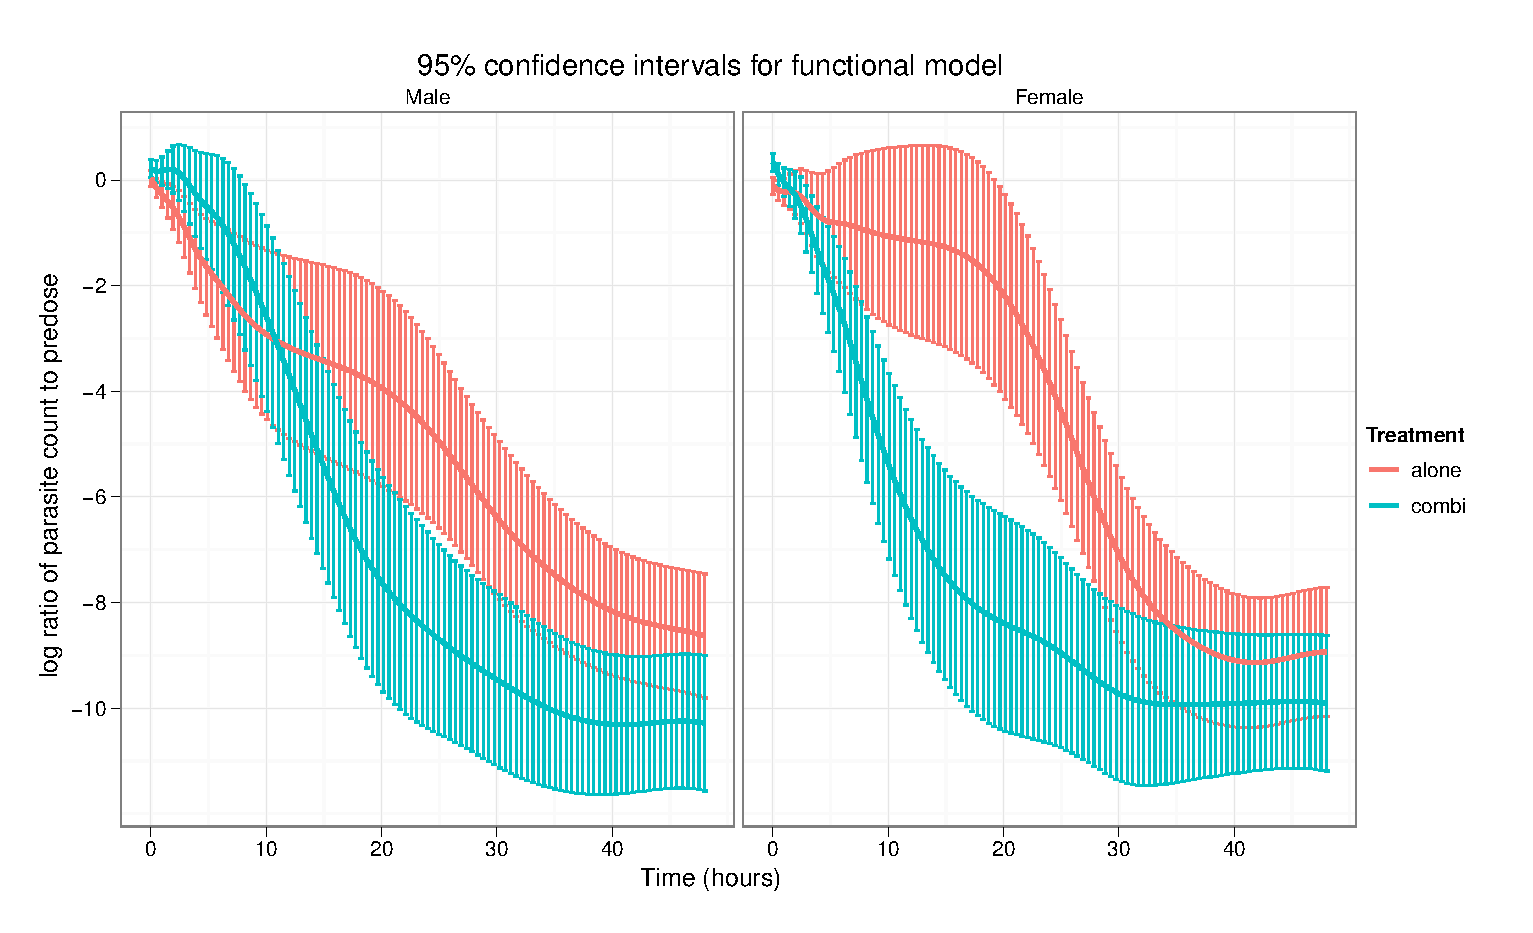
\includegraphics[width=150mm]{fdfitted.eps} 
\caption{Fitted count-ratio functions with confidence intervals}
\label{fdfitted}
\end{figure}

It can be seen that the difference between male subjects on the alone and combined drug treatment becomes large (relative to their 95\% confidence limits) between 20 and 30 hours reflecting the treatment effect shown in Figure \ref{fdcoef} between 20 and 30 hours. The difference between treatments for female subjects is larger between 10 and 30 hours reflecting the effect the sex-treatment interaction whereby the treatment effect is largest for female subjects. With reference to the 95\% confidence intervals, there is good evidence to reject the hypothesis that there is no effect of sex and treatment. The $F$ test in Figure \ref{fdapermF} is a more formal evaluation of this evidence. It would be useful to plot the difference between treatments, but calculation of the appropriate confidence intervals would require investigation of the correlation structure of the functional estimates, which has not been possible due to time constraints.

If we look again at Figure \ref{fdfitted}, we can see that although the parasite reduction is comparable (confidence intervals almost fully overlap) between treatments for male subjects, it is clear that the profiles have very different slopes between treatments; similarly for female patients, although the actual reduction level is also different. With functional data analysis it is easy to look, not only at the effect of factors on the response variable function, but also at the effect on derivatives of the response function. Accordingly, the functional ANOVA was repeated, but this time with the first derivative of the log count-ratio cubic spline functions. This fitted model is shown in Figure \ref{fdspeed}. 
\begin{figure}[p]
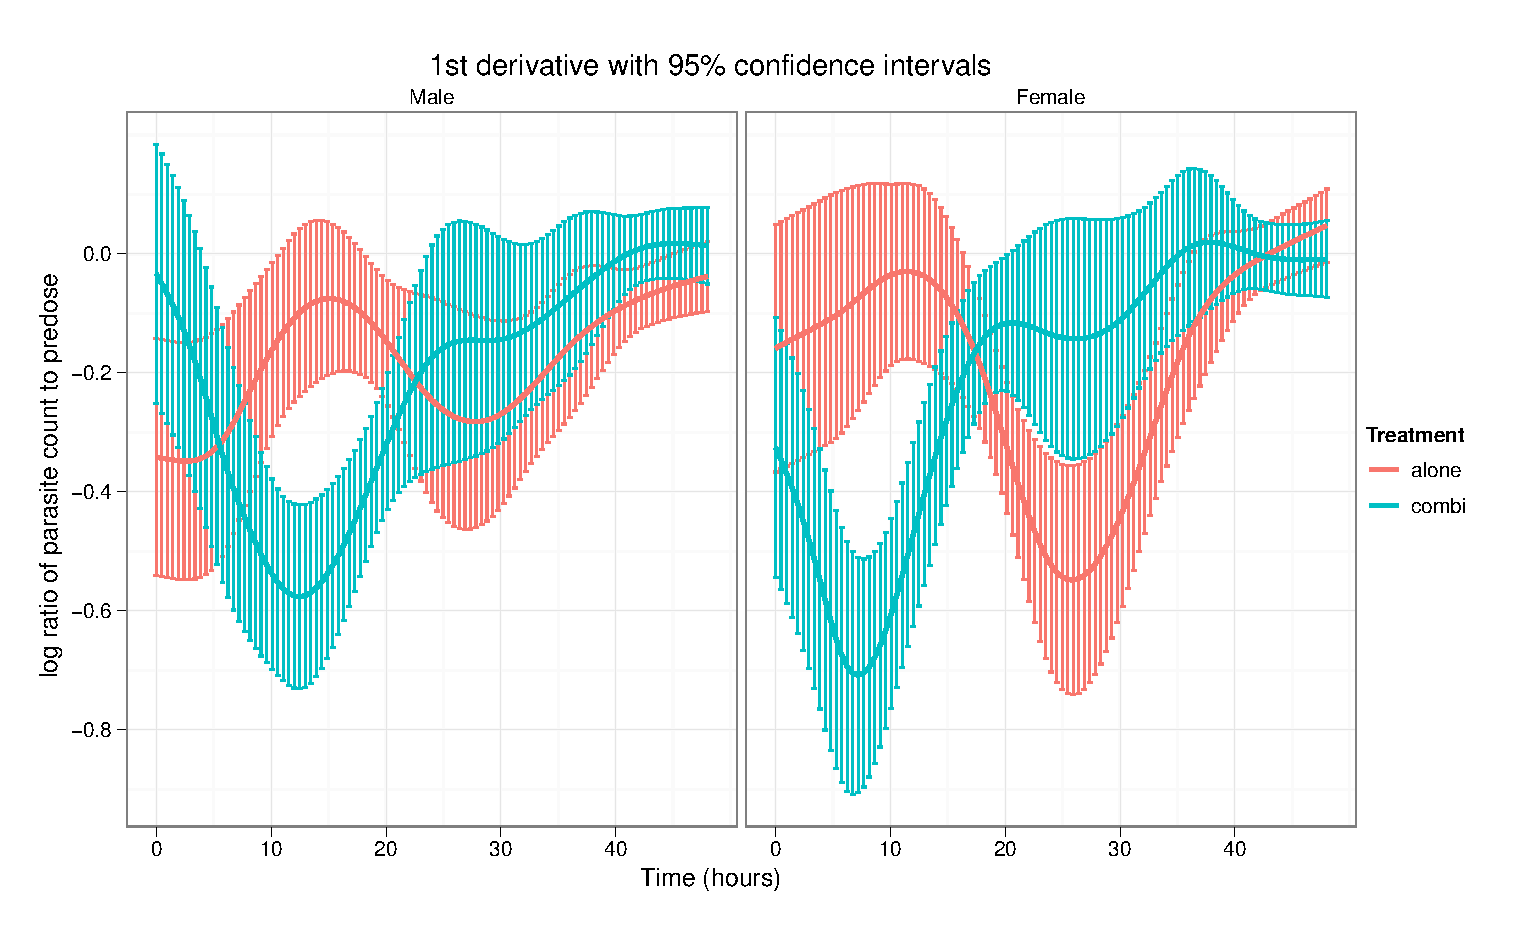
\includegraphics[width=150mm]{fdspeed.eps} 
\caption{Fitted functional model for 1st derivative of count ratio showing the effect of treatment on the instantaneous \emph{speed} of parasite clearance}
\label{fdspeed}
\end{figure}

It can be seen that the initial \emph{speed} of reduction is significantly faster (larger negative magnitude) from 10 to 15 hours for the combined treatment for both sexes, whereas the level of reduction (Figure \ref{fdfitted}) is not significantly different for male subjects up to at least 20 hours. What we can see from Figure \ref{fdspeed} is that the parasite-killing effect doesn't ``kick in'' and reach its maximum speed of parasite reduction until around 25 hours from first dose for the alone treatment, as opposed to around 10 hours for the combined treatment.

\clearpage
\section{Key results}
In this chapter some alternative methods of looking at how the parasite clearance is affected by experimental factors were explored. The key findings are:
\begin{itemize}
\item There is marginal evidence ($0.05<P<0.1$) to reject the hypothesis that there is no effect of a sex-treatment interaction on the time for half the parasites to be cleared from the blood (PC50). The reduction in PC50 clearance time for female patients on the combined treatment over the single treatment is 7.1 hours with a 95\% confidence interval of (0.7, 9.9) hours. There is no evidence to reject the hypothesis that PC50 clearance times are the same for male subjects on either treatment.
\item There is good evidence ($P<0.0005$) to reject the hypothesis that treatment has no effect on the time for 99\% of parasites to be cleared from the blood (PC99). The result of this hypothesis test is not altered when lower and upper extreme estimates are made for 3 subjects for whom PC99 was not achieved within the time period of the trial. The reduction in PC99 for subjects on the combined treatment is 12.1 hours with a 95\% confidence interval of (7.5, 16.9) hours.
\item The technique of functional data analysis was applied to this data whereby the parasite count profiles are described by smooth cubic-spline functions. The functional equivalent of ANOVA was then performed on these splines by sex and treatment. This gave evidence to reject the hypothesis that treatment has no effect on the parasite count between 17 and 45 hours from first dose and evidence to reject the hypothesis that there is no interaction between sex and treatment that affects the parasite count between 10 and 15 hours.
\item The maximum speed of parasite reduction is obtained for the combined treatment around 15 hours before the single treatment.
\end{itemize}
\chapter{Discussion}\label{ch:discussion}
The were two primary questions addressed in this dissertation.
\begin{enumerate}
\item Given profiles of parasite counts per microlitre of blood with time from first dose of an antimalarial treatment, how do we derive an estimate of the time taken for 90\% of the parasites to be cleared from the blood?
\item Given our estimated times for parasite clearance, how do we determine if the average clearance time for subjects on one antimalarial treatment is significantly different to the average clearance time for subjects on an alternative treatment?
\end{enumerate}
The first question is not really one that can be formulated as a statistical hypothesis test, but is more a question of making a sensible and consistent estimate. The second question can be answered by the identification of a suitable test statistic.

The following discussion is primarily concerned with how these questions have been answered, but also goes on to look at some of the wider issues raised concerning analysis of data of this type.

\section{Derivation of clearance times}

\subsection{The nature of the problem}
In order to estimate the time for the parasite count to reach 90\% of its pre-dose level we need to know the nature of how the parasite count changes with time. Whether it falls monotonically, for example, follows a linear, or more complicated trend. The observed behaviours were summarised in section \ref{sec:behaviours} and can be seen in Figures \ref{raw1} and \ref{raw2} on pages \pageref{raw1} and \pageref{raw2}. One problem with this data is that we do not know how much of the erratic variation in parasite count per microlitre recorded genuinely reflects a sharp change in the parasite load of the subject and how much is due to error in the counting procedure. It is reported for patients taking antimalarial drugs that ``\textit{parasitemia may rise alarmingly in the hours following treatment}'' \cite{white}. However, it was reported by our contact at GSK that there may be a large variability in parasite counts simply due to the choice of the ``suitable'' area of the blood sample slide chosen by microscopists for parasite counting. Nevertheless, it seems that in the region around the PC90 level that the fall in parasite count is fairly smooth and not nearly as erratic as at earlier times. This can be seen in Figure \ref{comprawlog} on \pageref{comprawlog}. Hence, it seems that estimation between data recording times is more predictable in the PC90 region than at earlier times and that early erratic variation in the count is irrelevant. In this respect PC90 would seem a sensible choice of endpoint.
\subsection{Choice of interpolation method}
\subsubsection*{Criticism of the choice of logistic modelling}
We were told by GSK that logistic modelling had already been used for PC90 estimation for this data and suggested aims for this dissertation were the investigation of the logistic approach such as how to choose appropriate starting parameters for the fitting. This was done, however it was found that the logistic model simply did not have the appropriate shape for modelling the parasite-count profiles of some subjects. It is also not clear as to why a model for the whole count profile must be fitted in order to make an estimate within a narrow time window between observations that bracket the time of interest. It could be argued that the two observations either side of the PC90 time could be subject to a relatively large error and therefore the behaviour should be averaged over a wider timescale. However, this could be more suitably achieved with some sort of spline regression as it seems innappropriate for large fluctuations at early times to influence the estimate at later times when the count profile is relatively smooth.

Some problems with logistic regression are highlighted by Wootton {\it et al.}  

\section{Analysis of clearance times}

\addappheadtotoc
\appendix
\appendixpage
\begin{singlespace}
\chapter{Complete plots of data}

\section{Raw parasite counts}\label{A:lograwcount}
On the following pages are the plots of the log parasite count per \micro\liter\ for all subjects with PC90 level shown. Each page contains the data for 1 centre and sex.
\begin{sidewaysfigure}
\centering
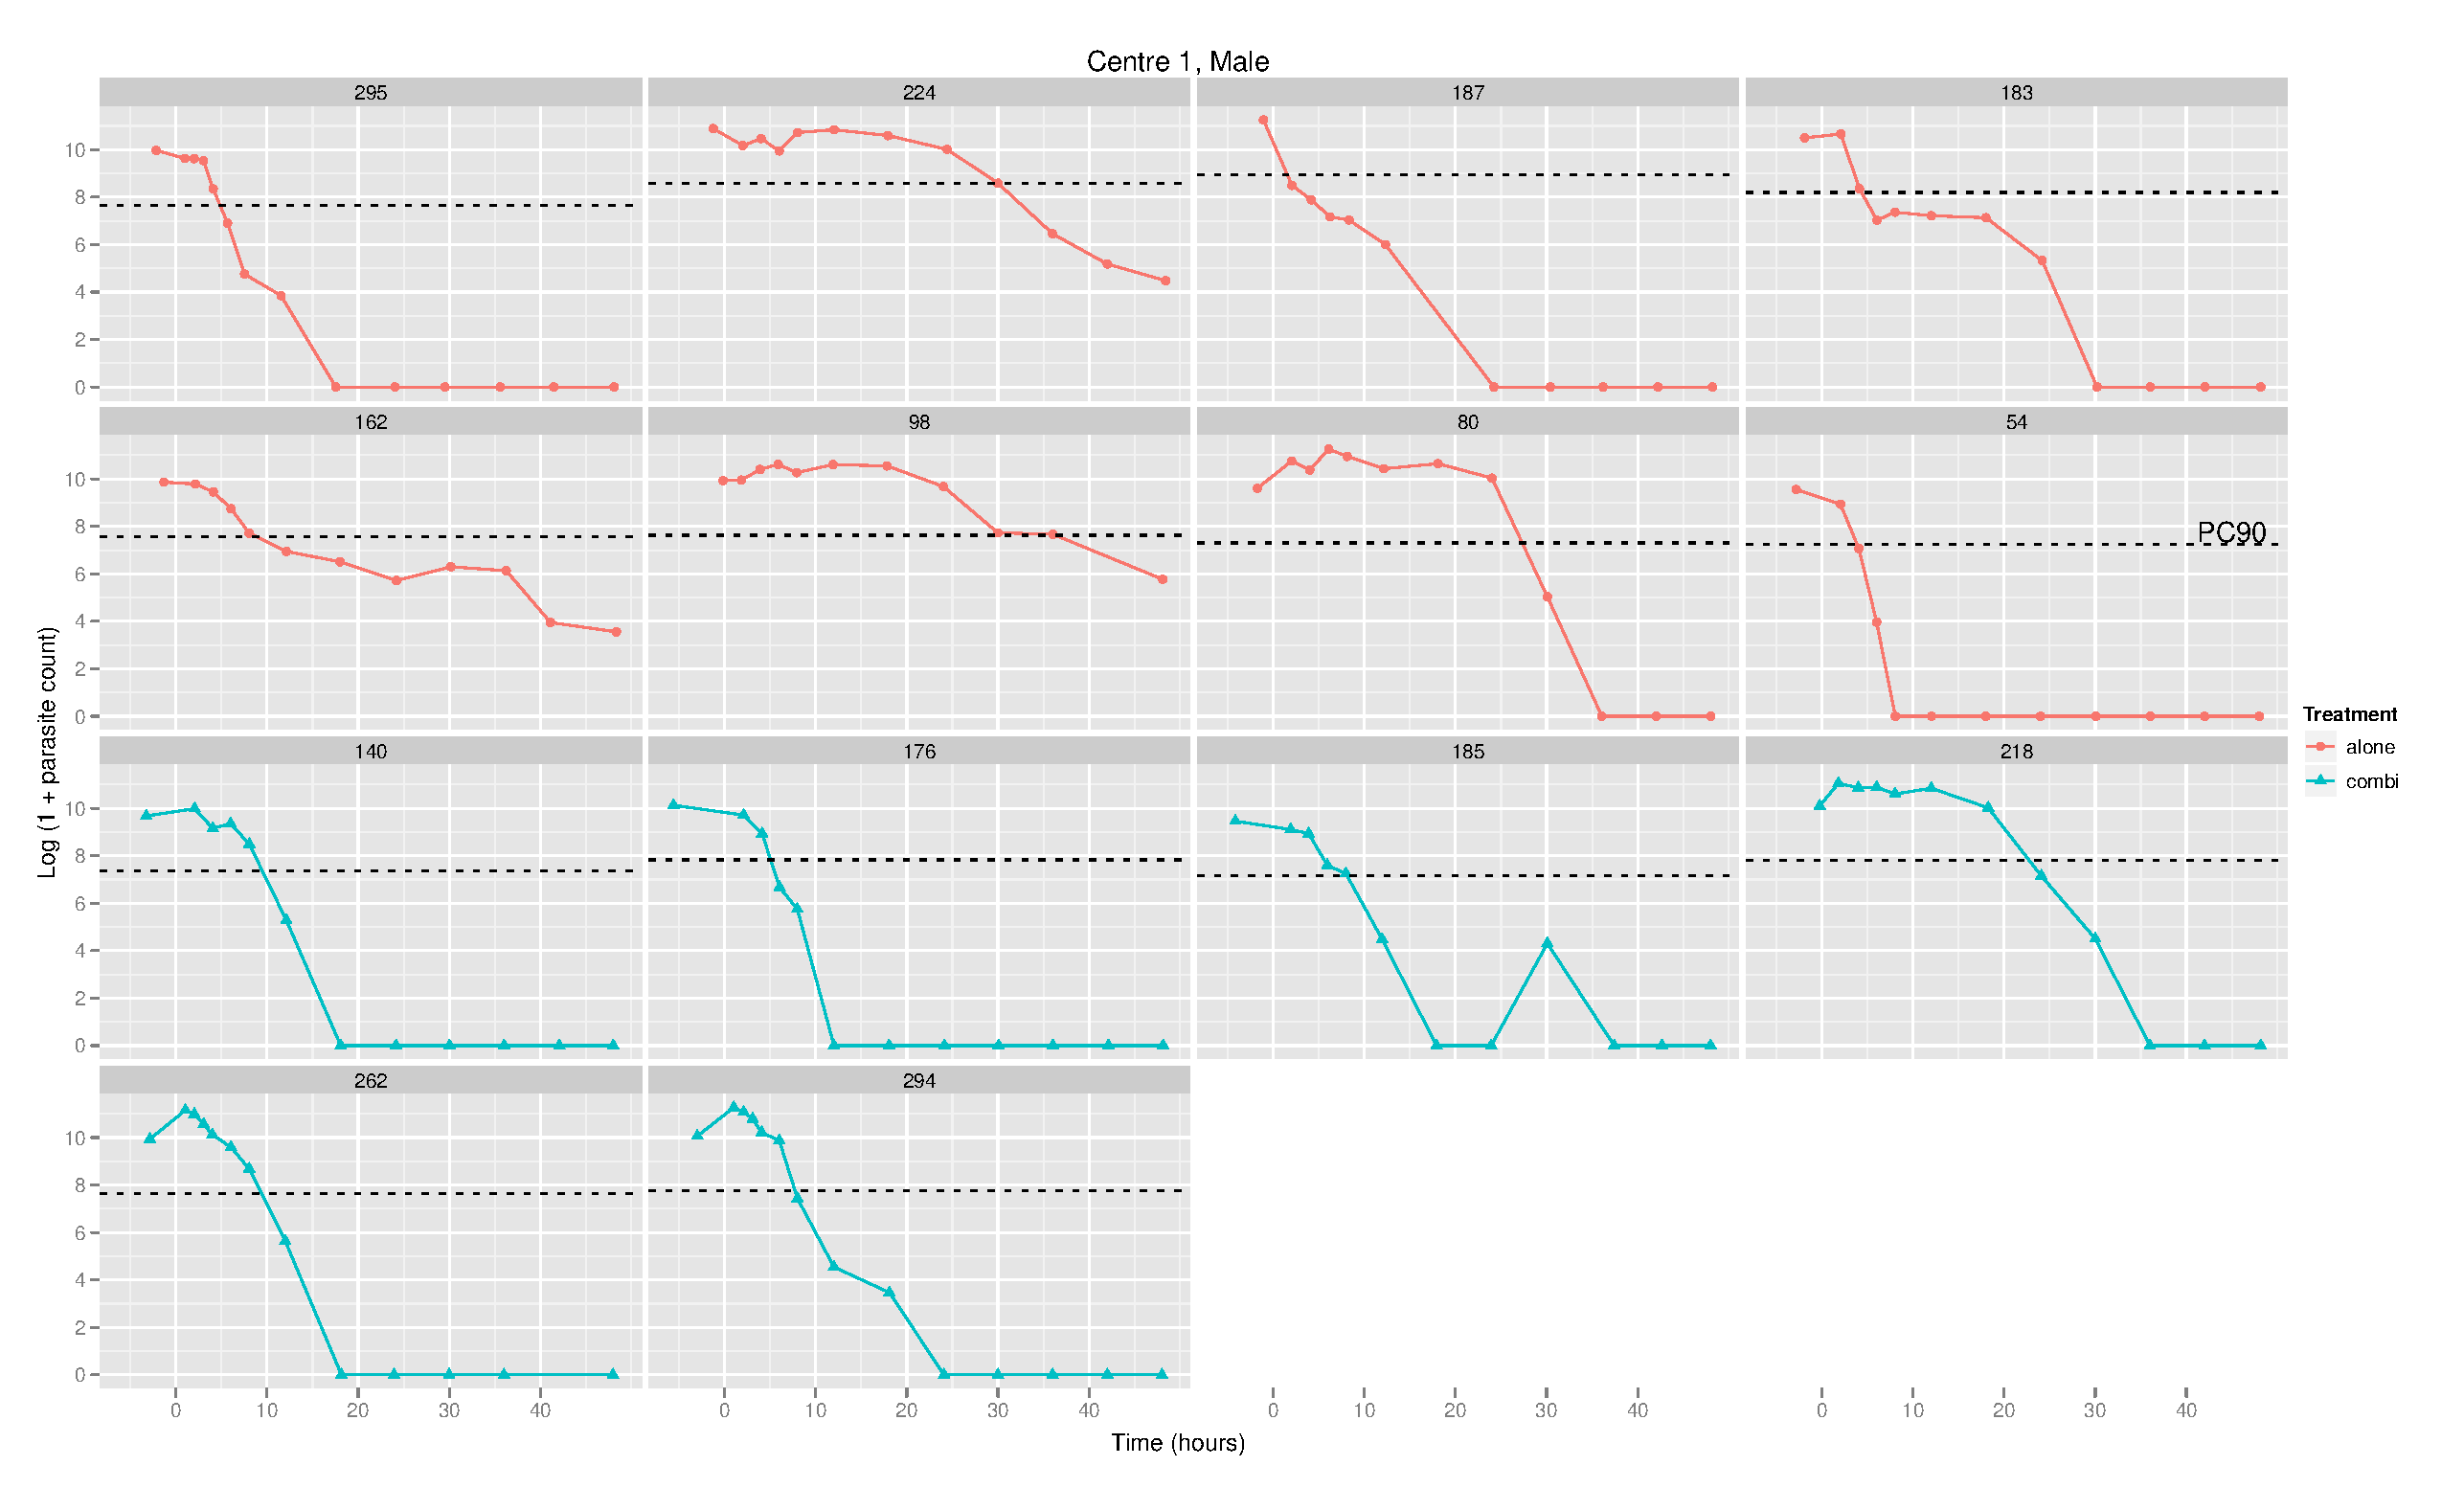
\includegraphics[height=150mm]{Araw1M.eps}
\end{sidewaysfigure}
\begin{sidewaysfigure}
\centering
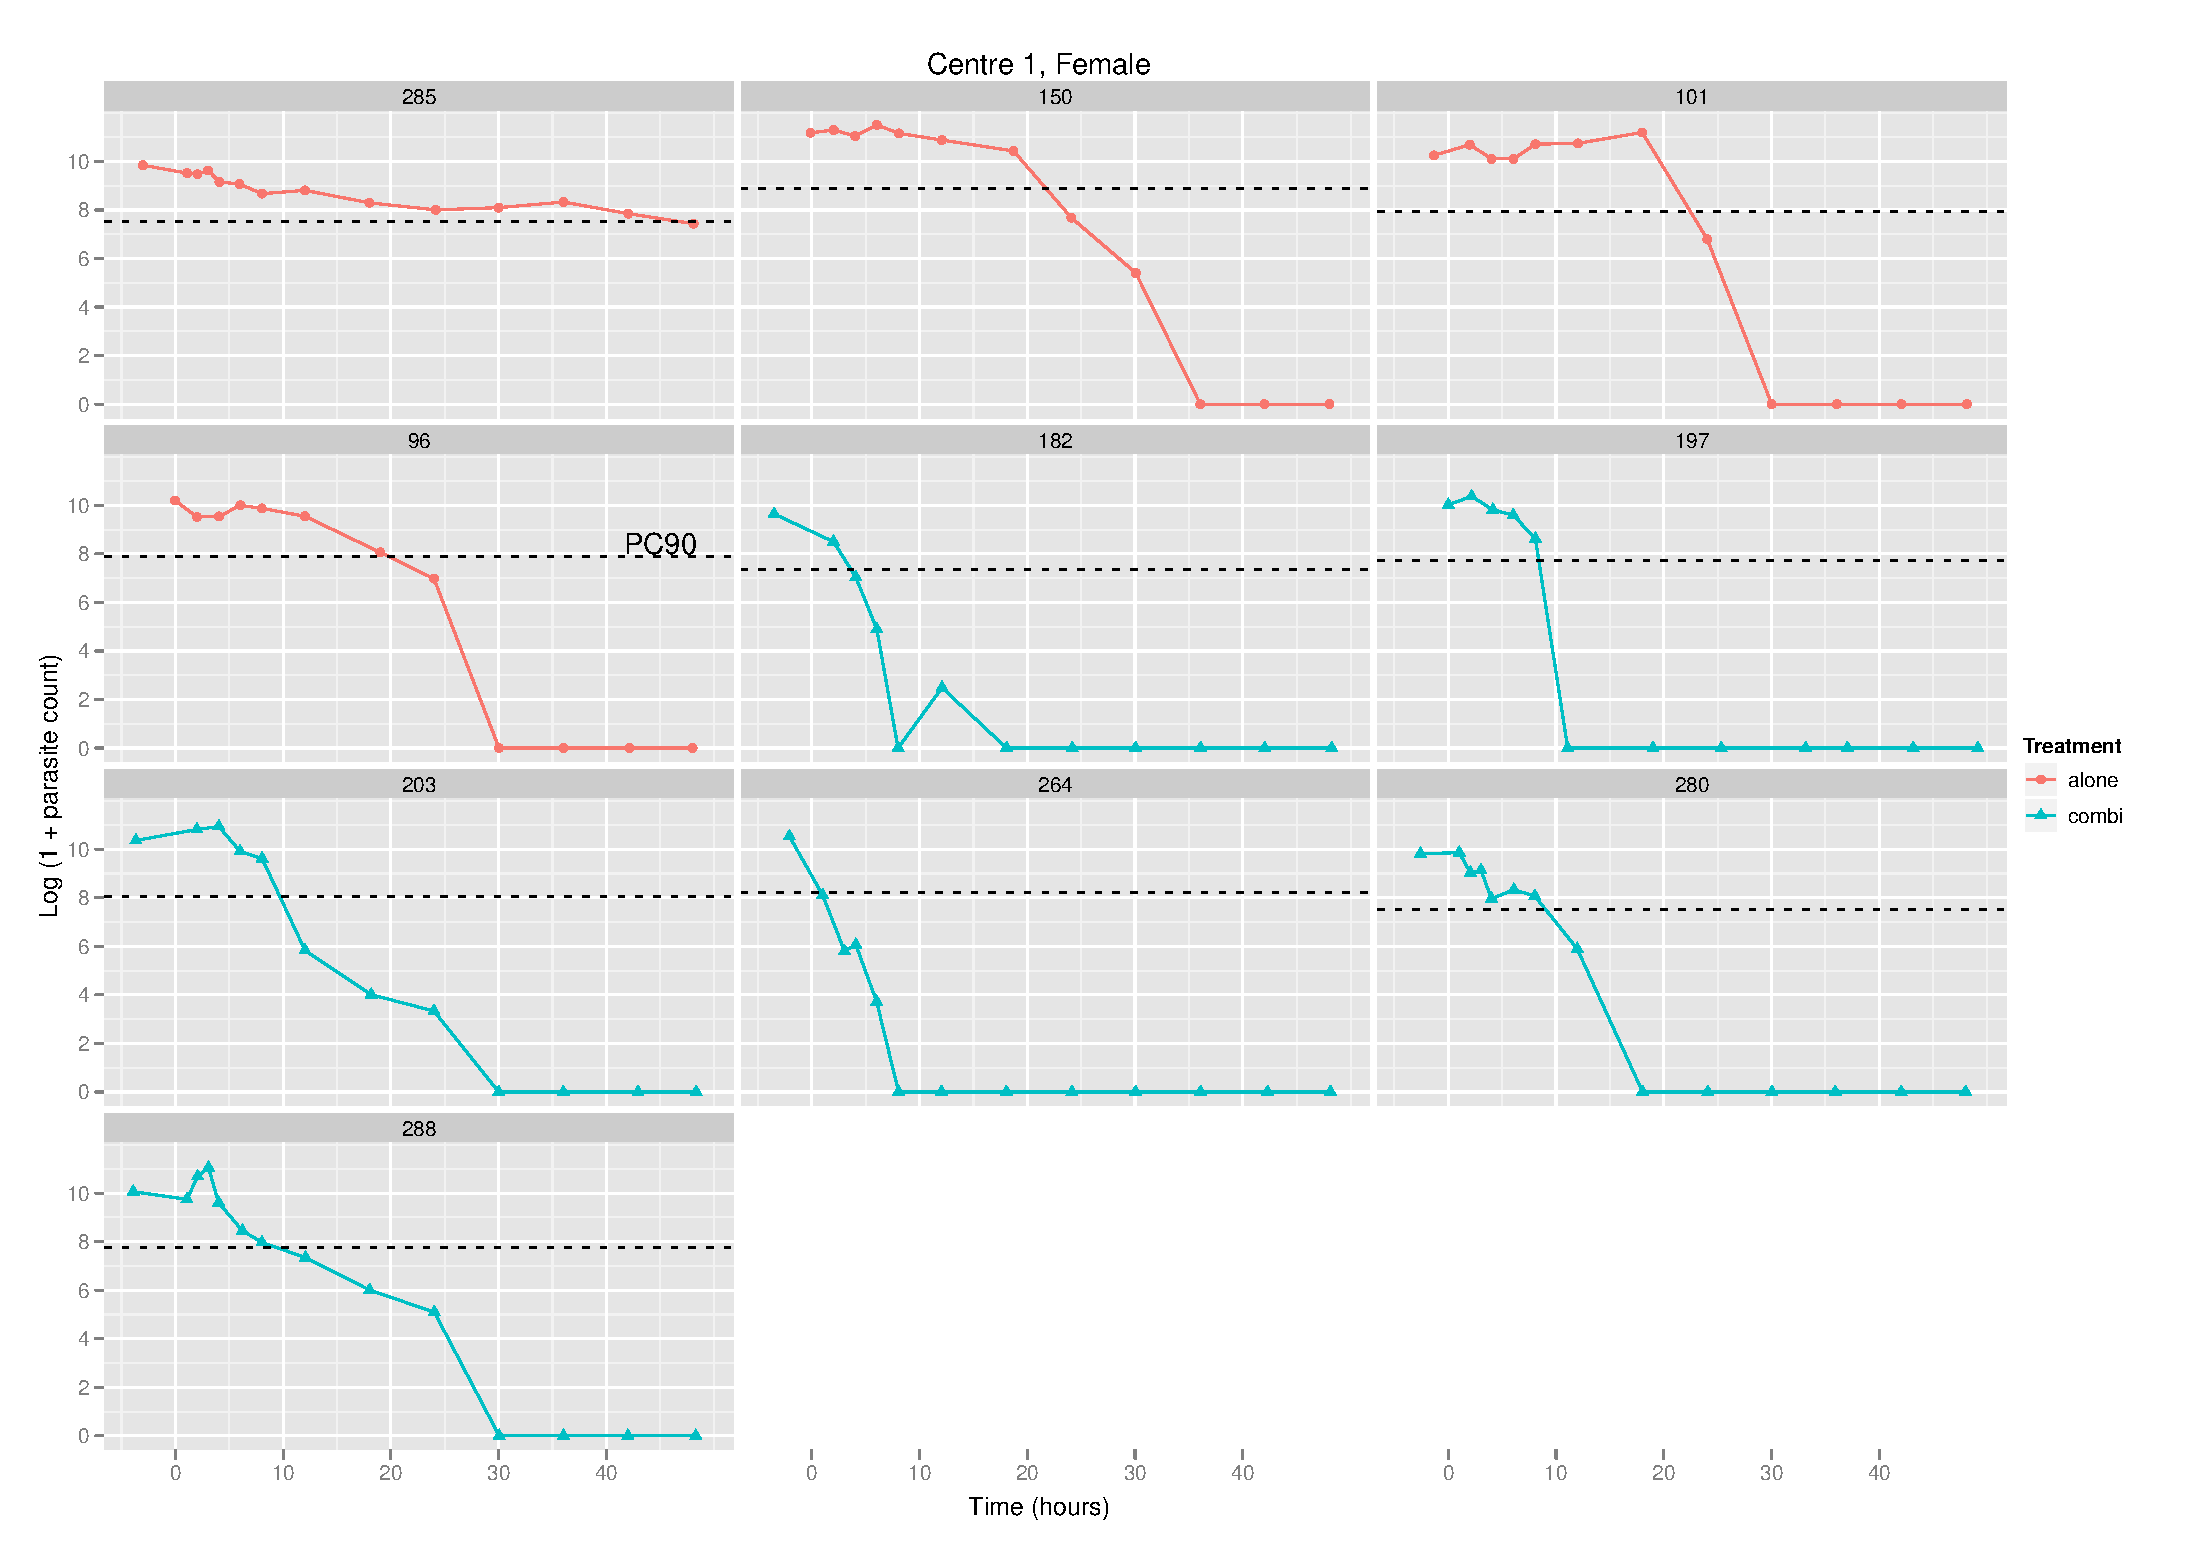
\includegraphics[height=150mm]{Araw1F.eps}
\end{sidewaysfigure}
\begin{sidewaysfigure}
\centering
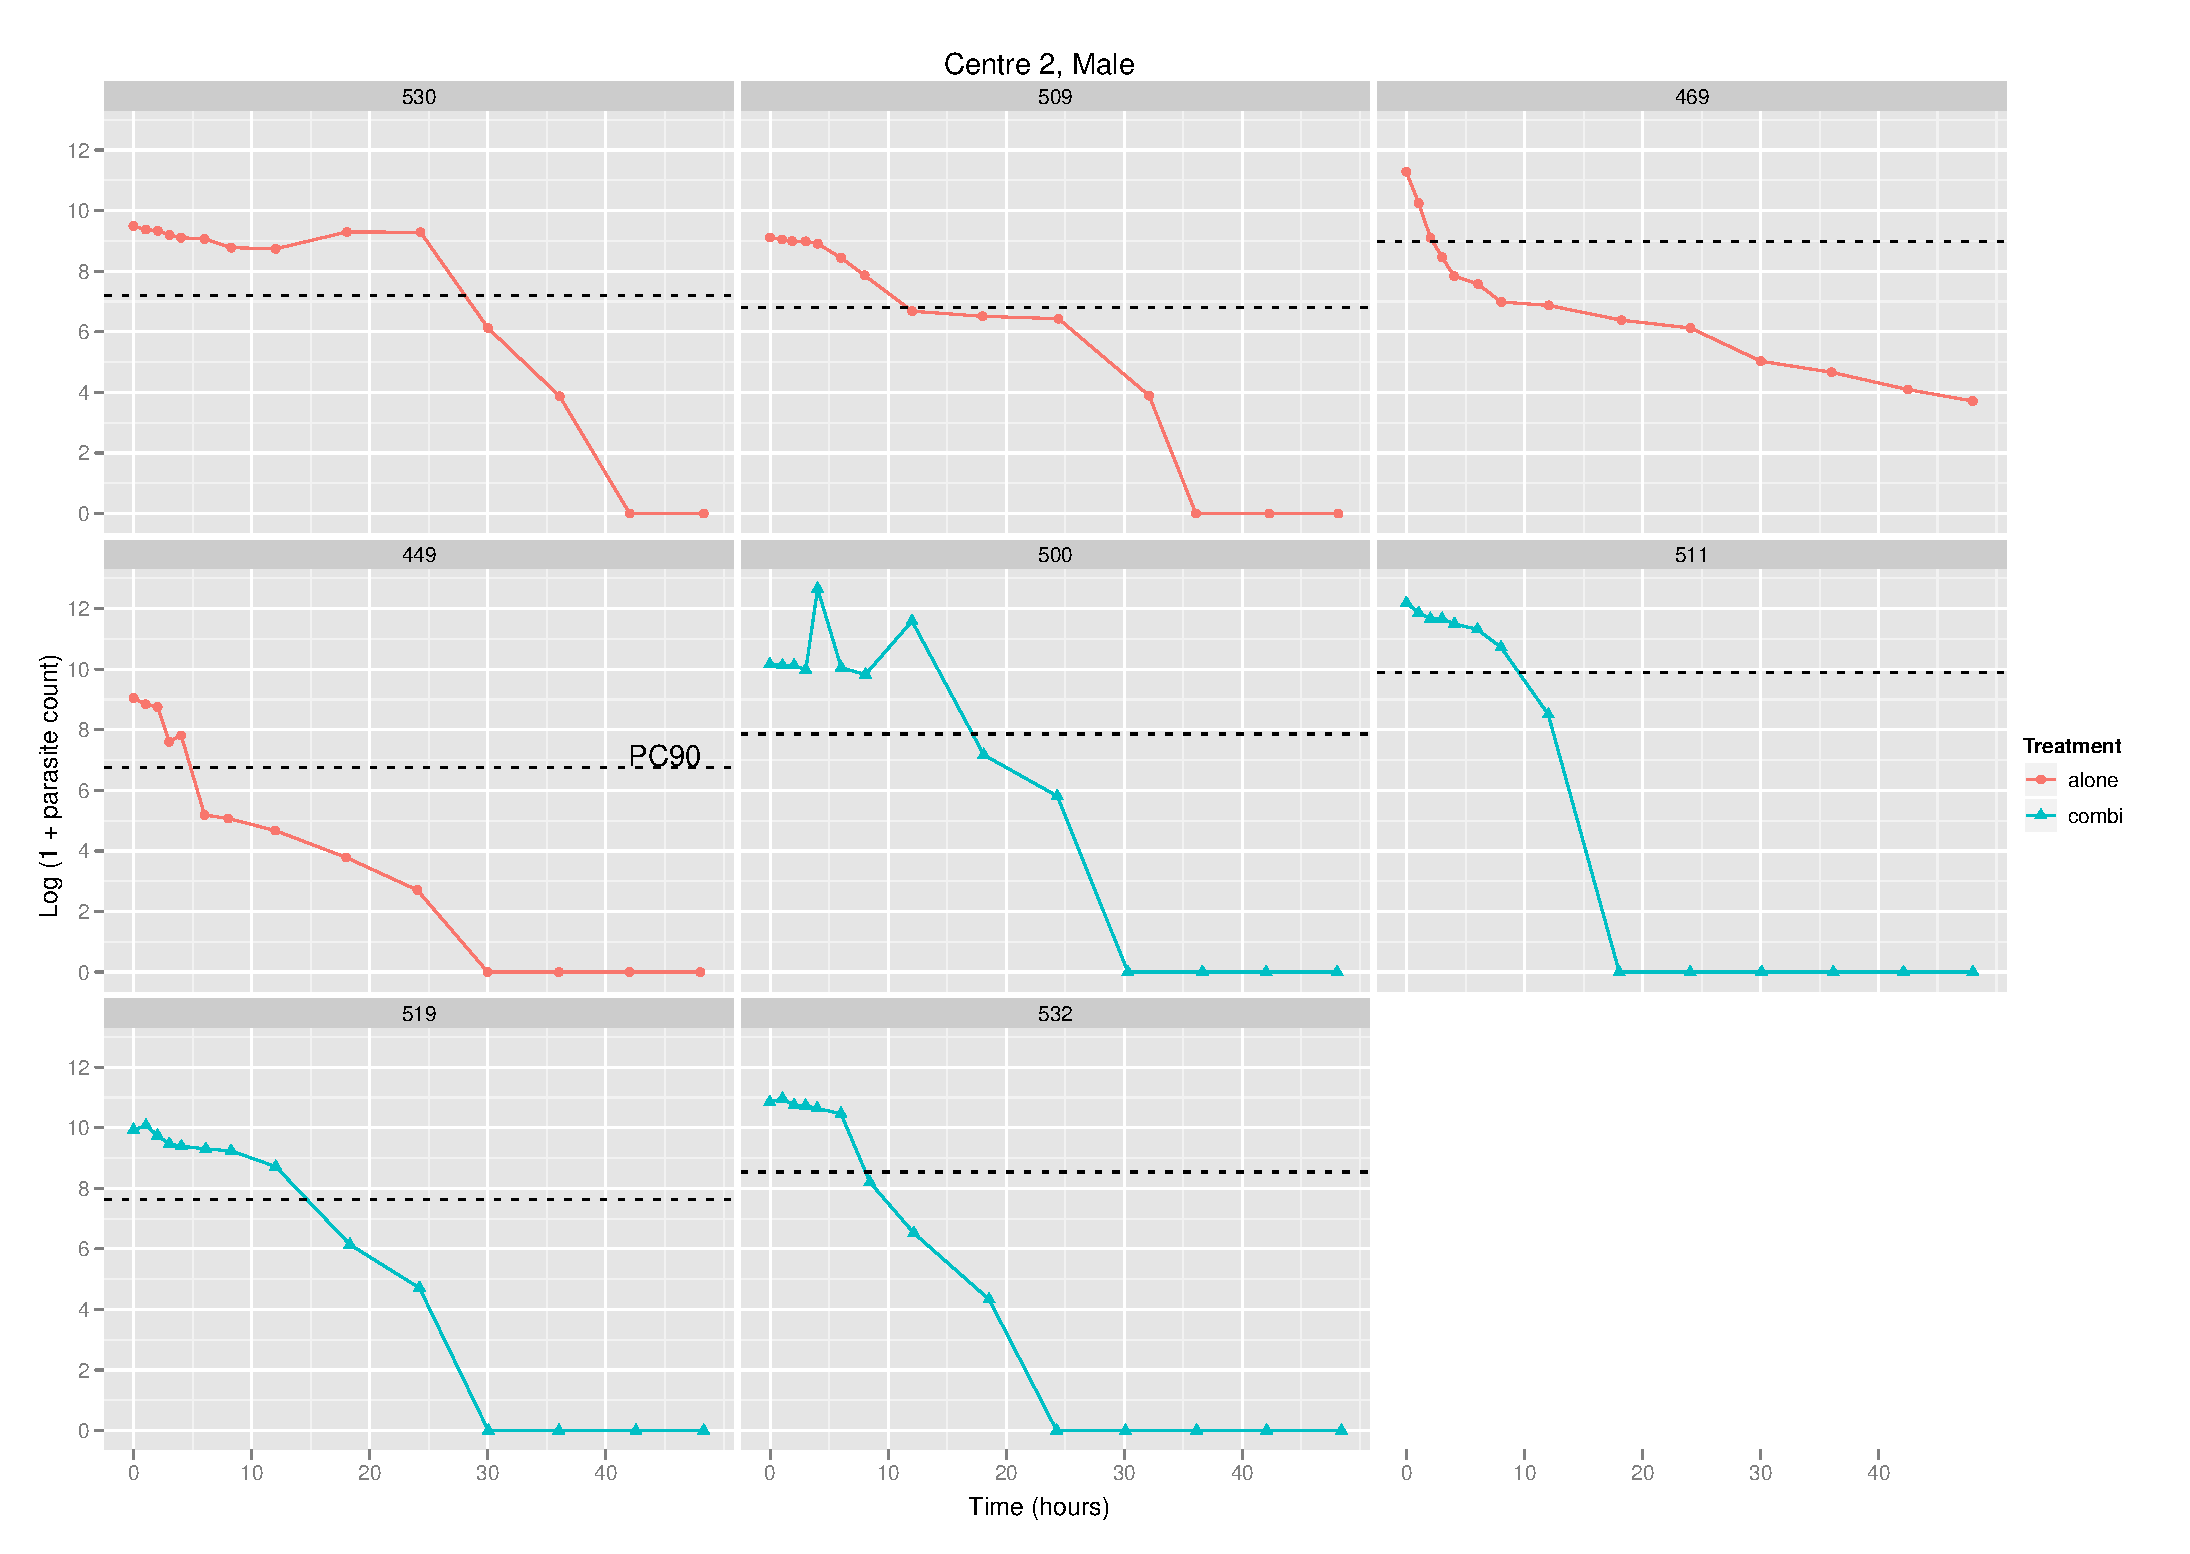
\includegraphics[height=150mm]{Araw2M.eps}
\end{sidewaysfigure}
\begin{sidewaysfigure}
\centering
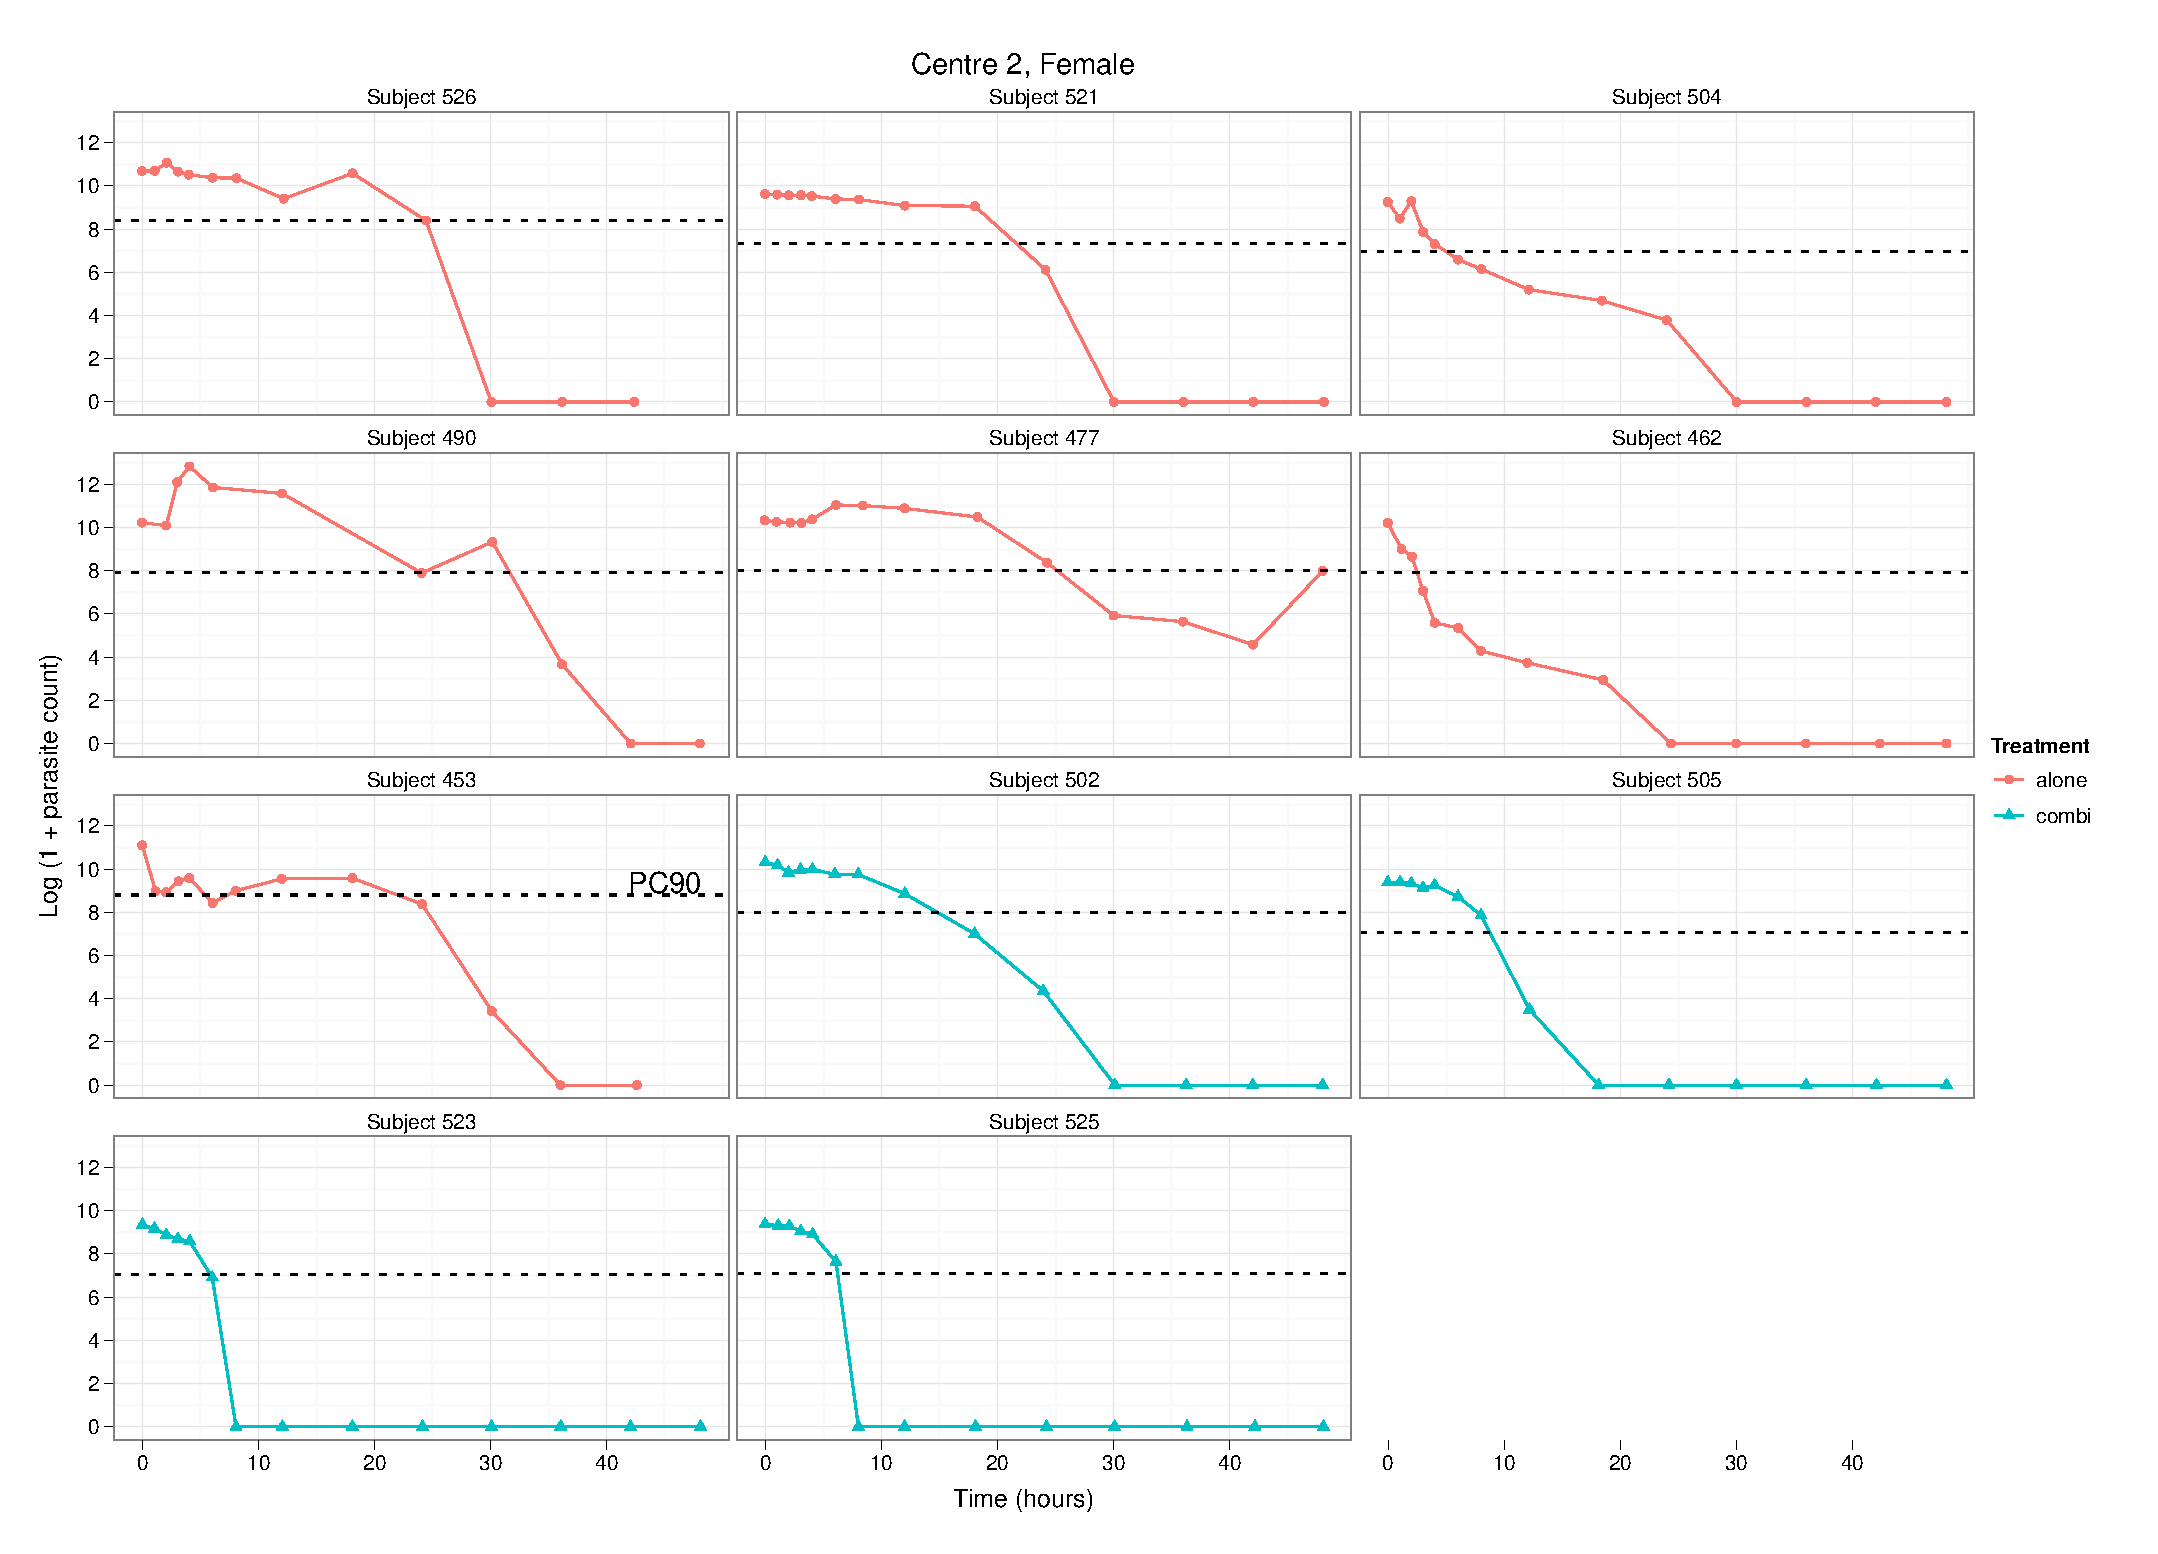
\includegraphics[height=150mm]{Araw2F.eps}
\end{sidewaysfigure}

\clearpage
\section{Model fits}\label{A:modelfits}
On the following pages are the model fits used for PC90 estimation for all subjects, with the PC90 time estimated by each method shown as a vertical line. Each page contains the data for 1 centre and sex.
\begin{sidewaysfigure}
\centering
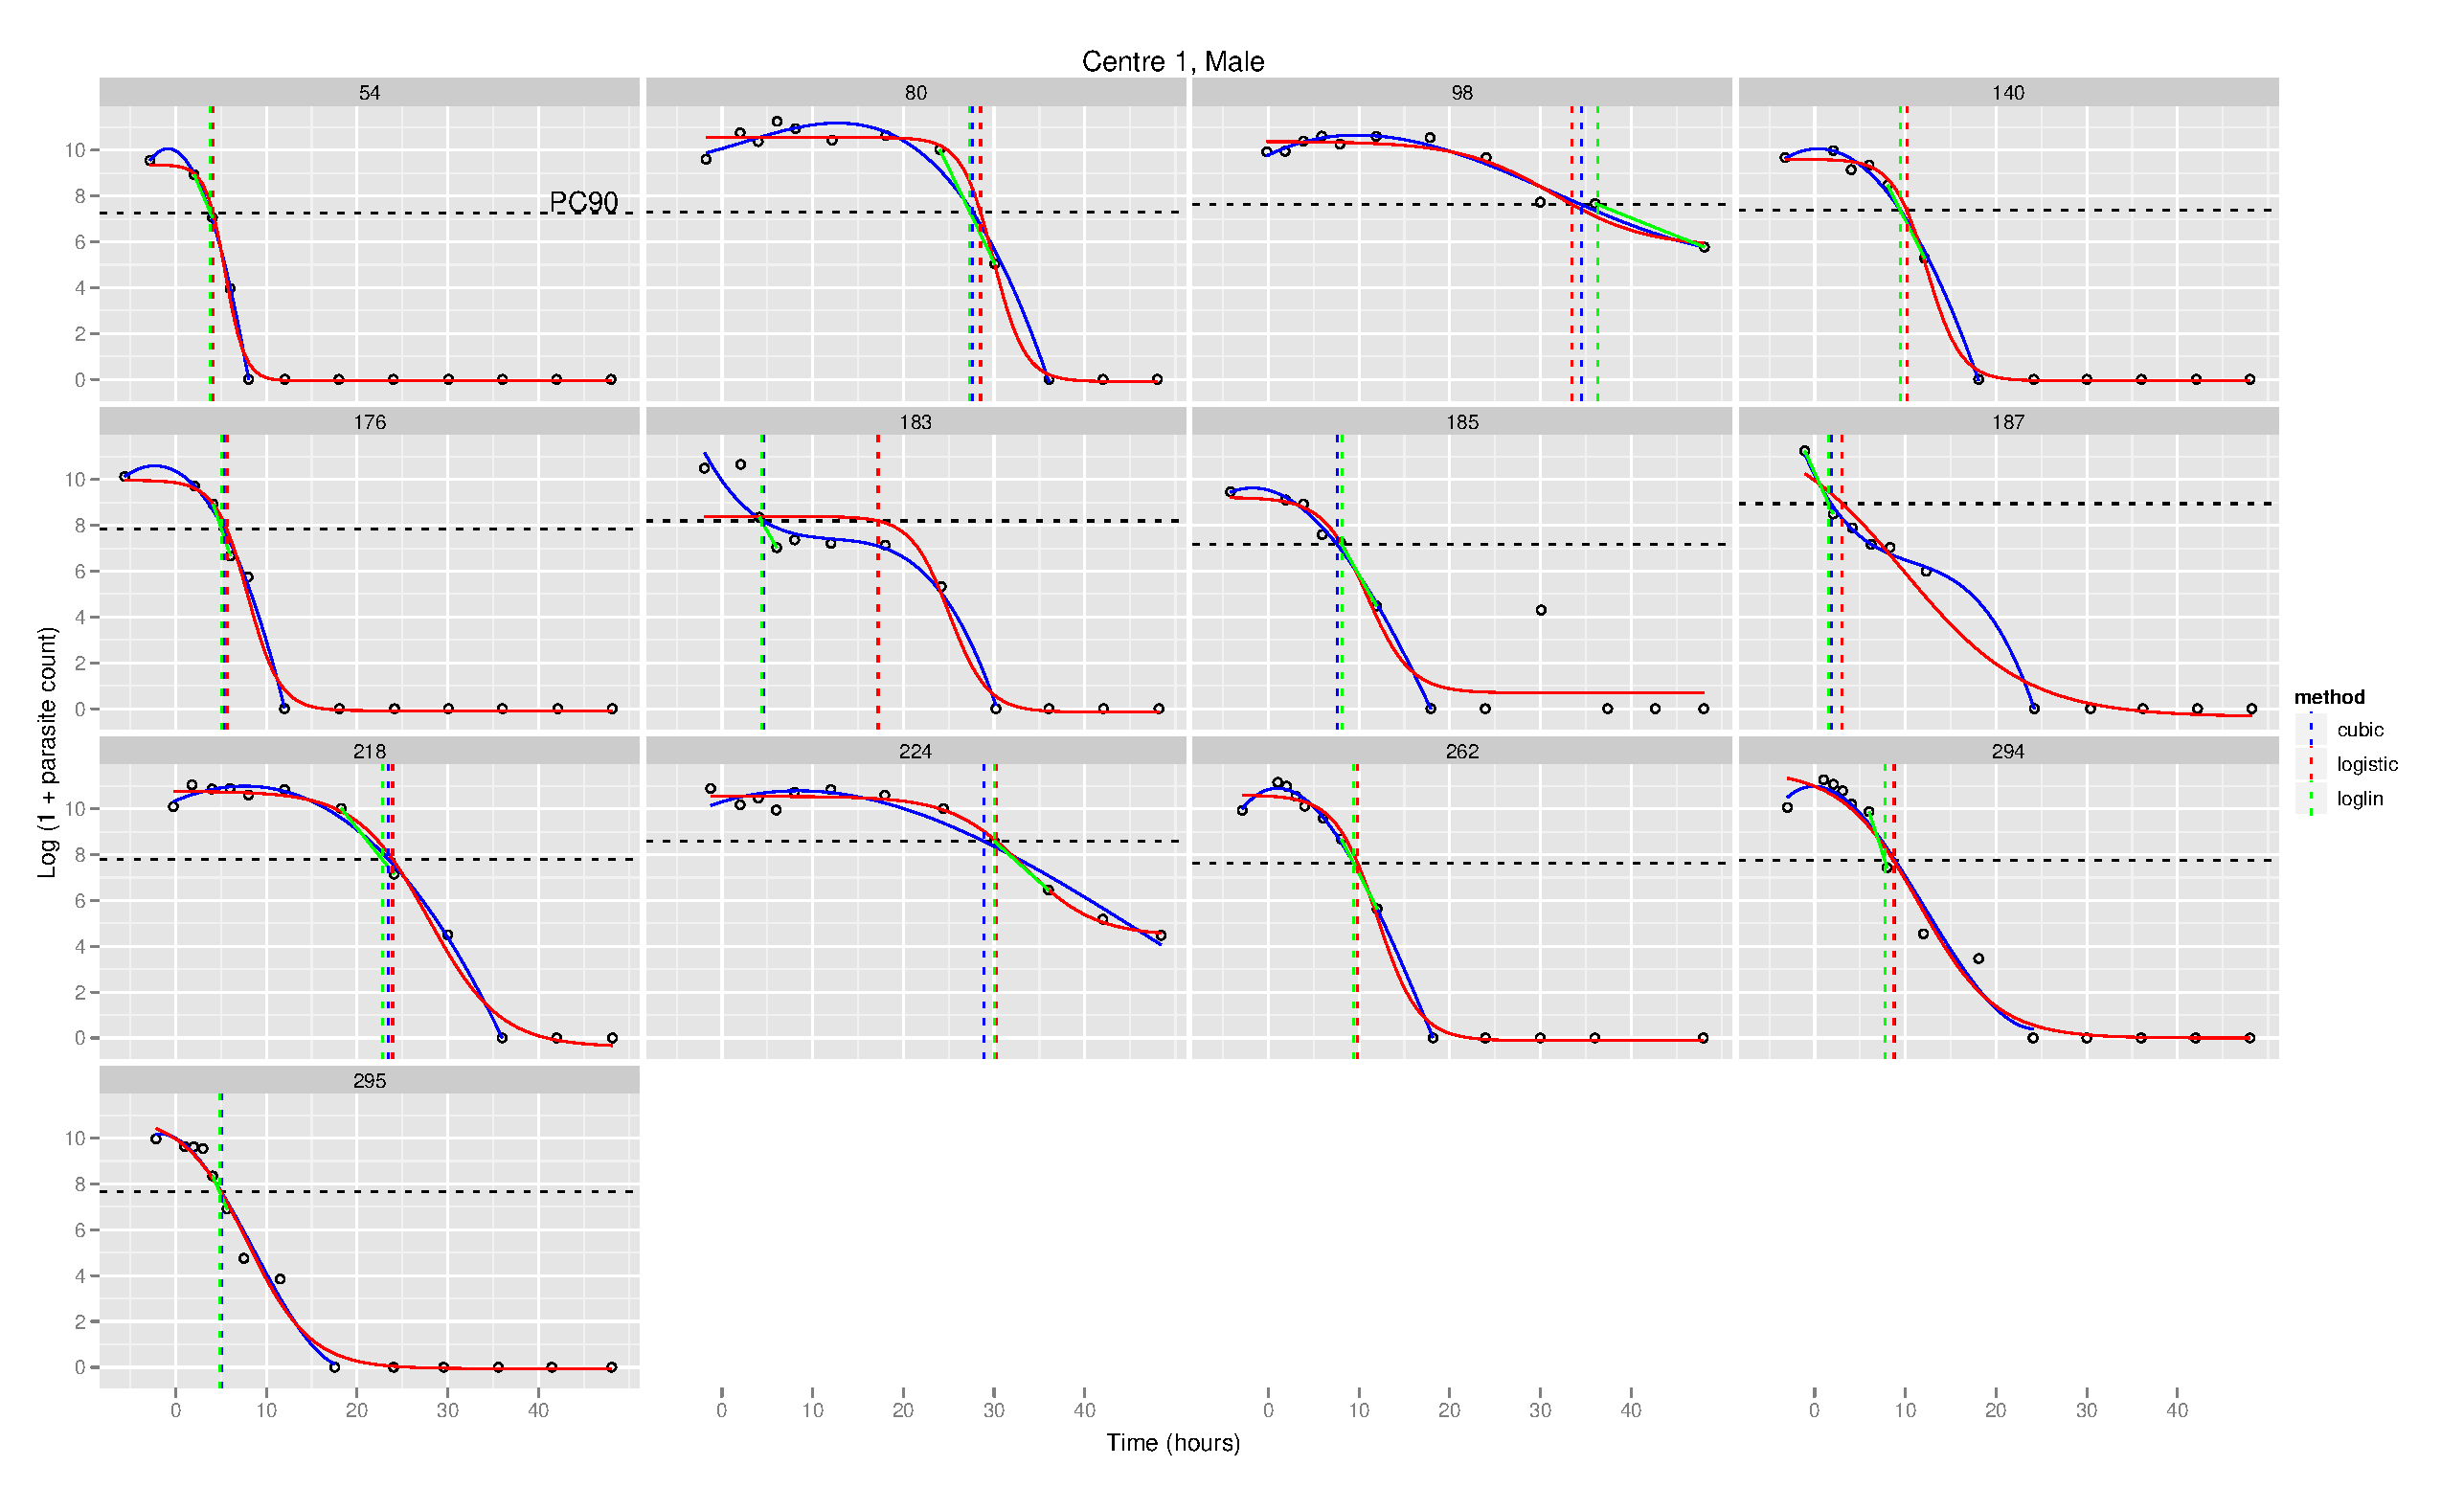
\includegraphics[height=150mm]{Afits1M.eps}
\end{sidewaysfigure}
\begin{sidewaysfigure}
\centering
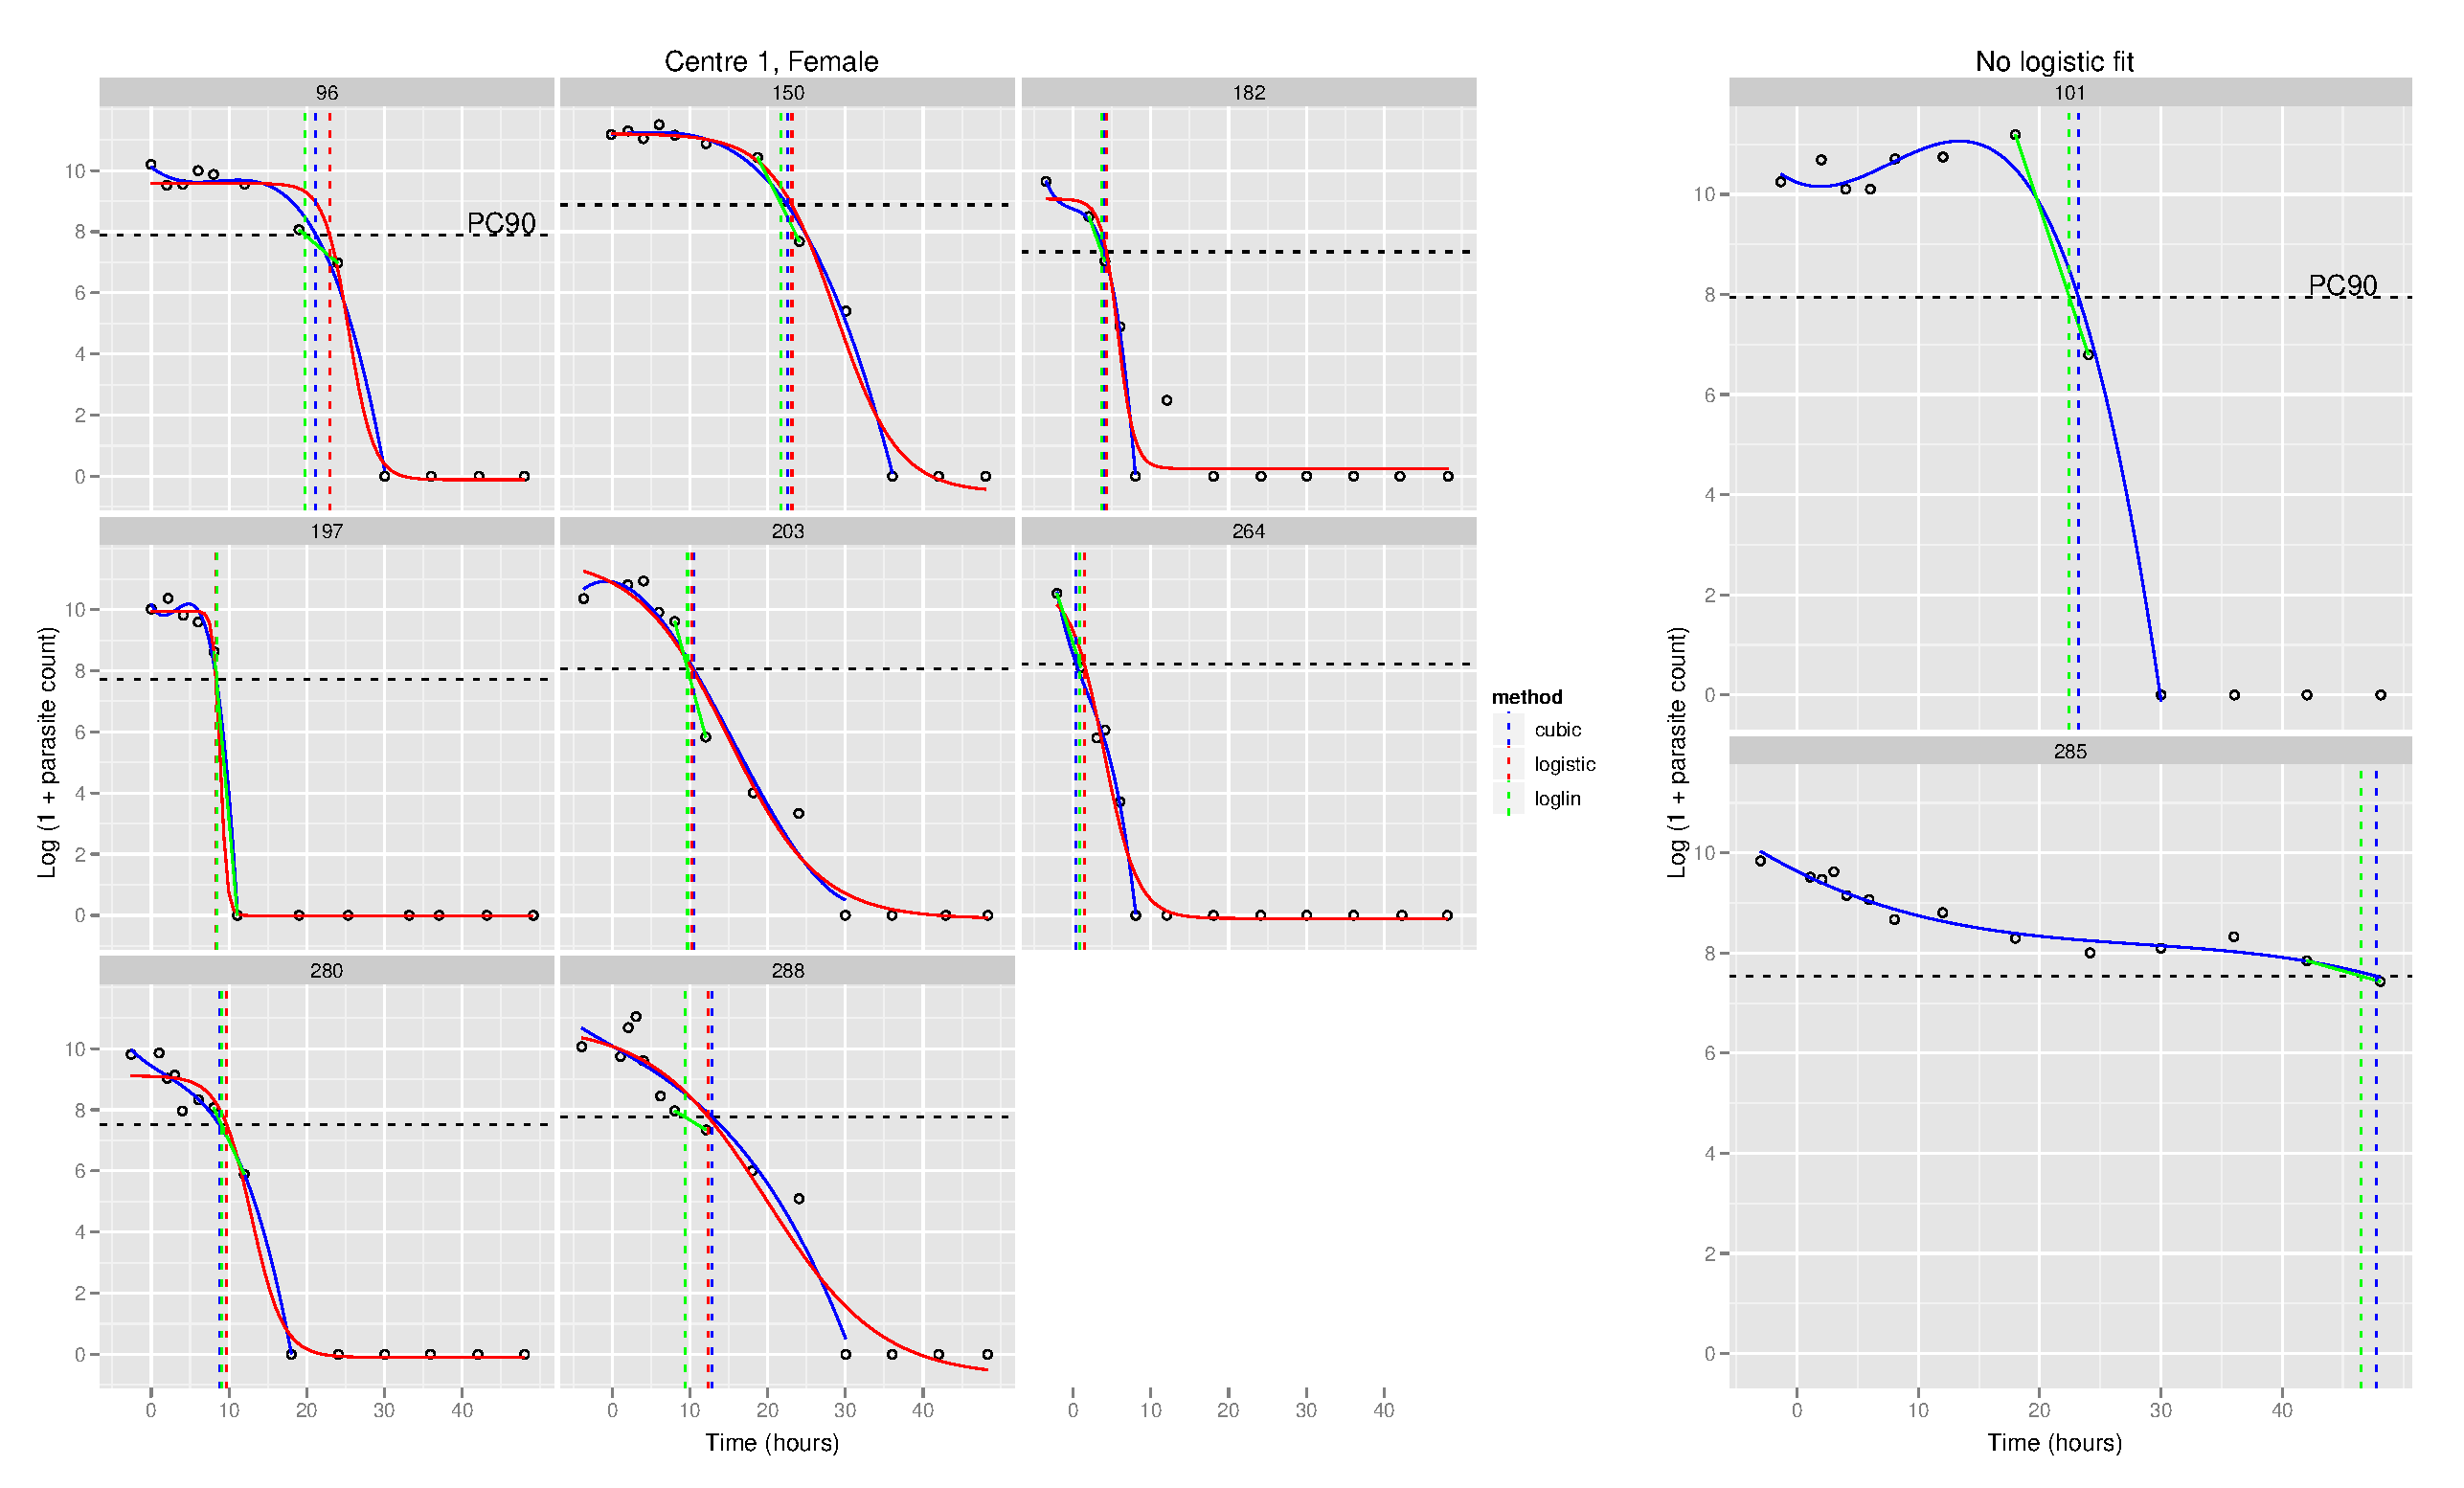
\includegraphics[height=150mm]{Afits1F.eps}
\end{sidewaysfigure}
\begin{sidewaysfigure}
\centering
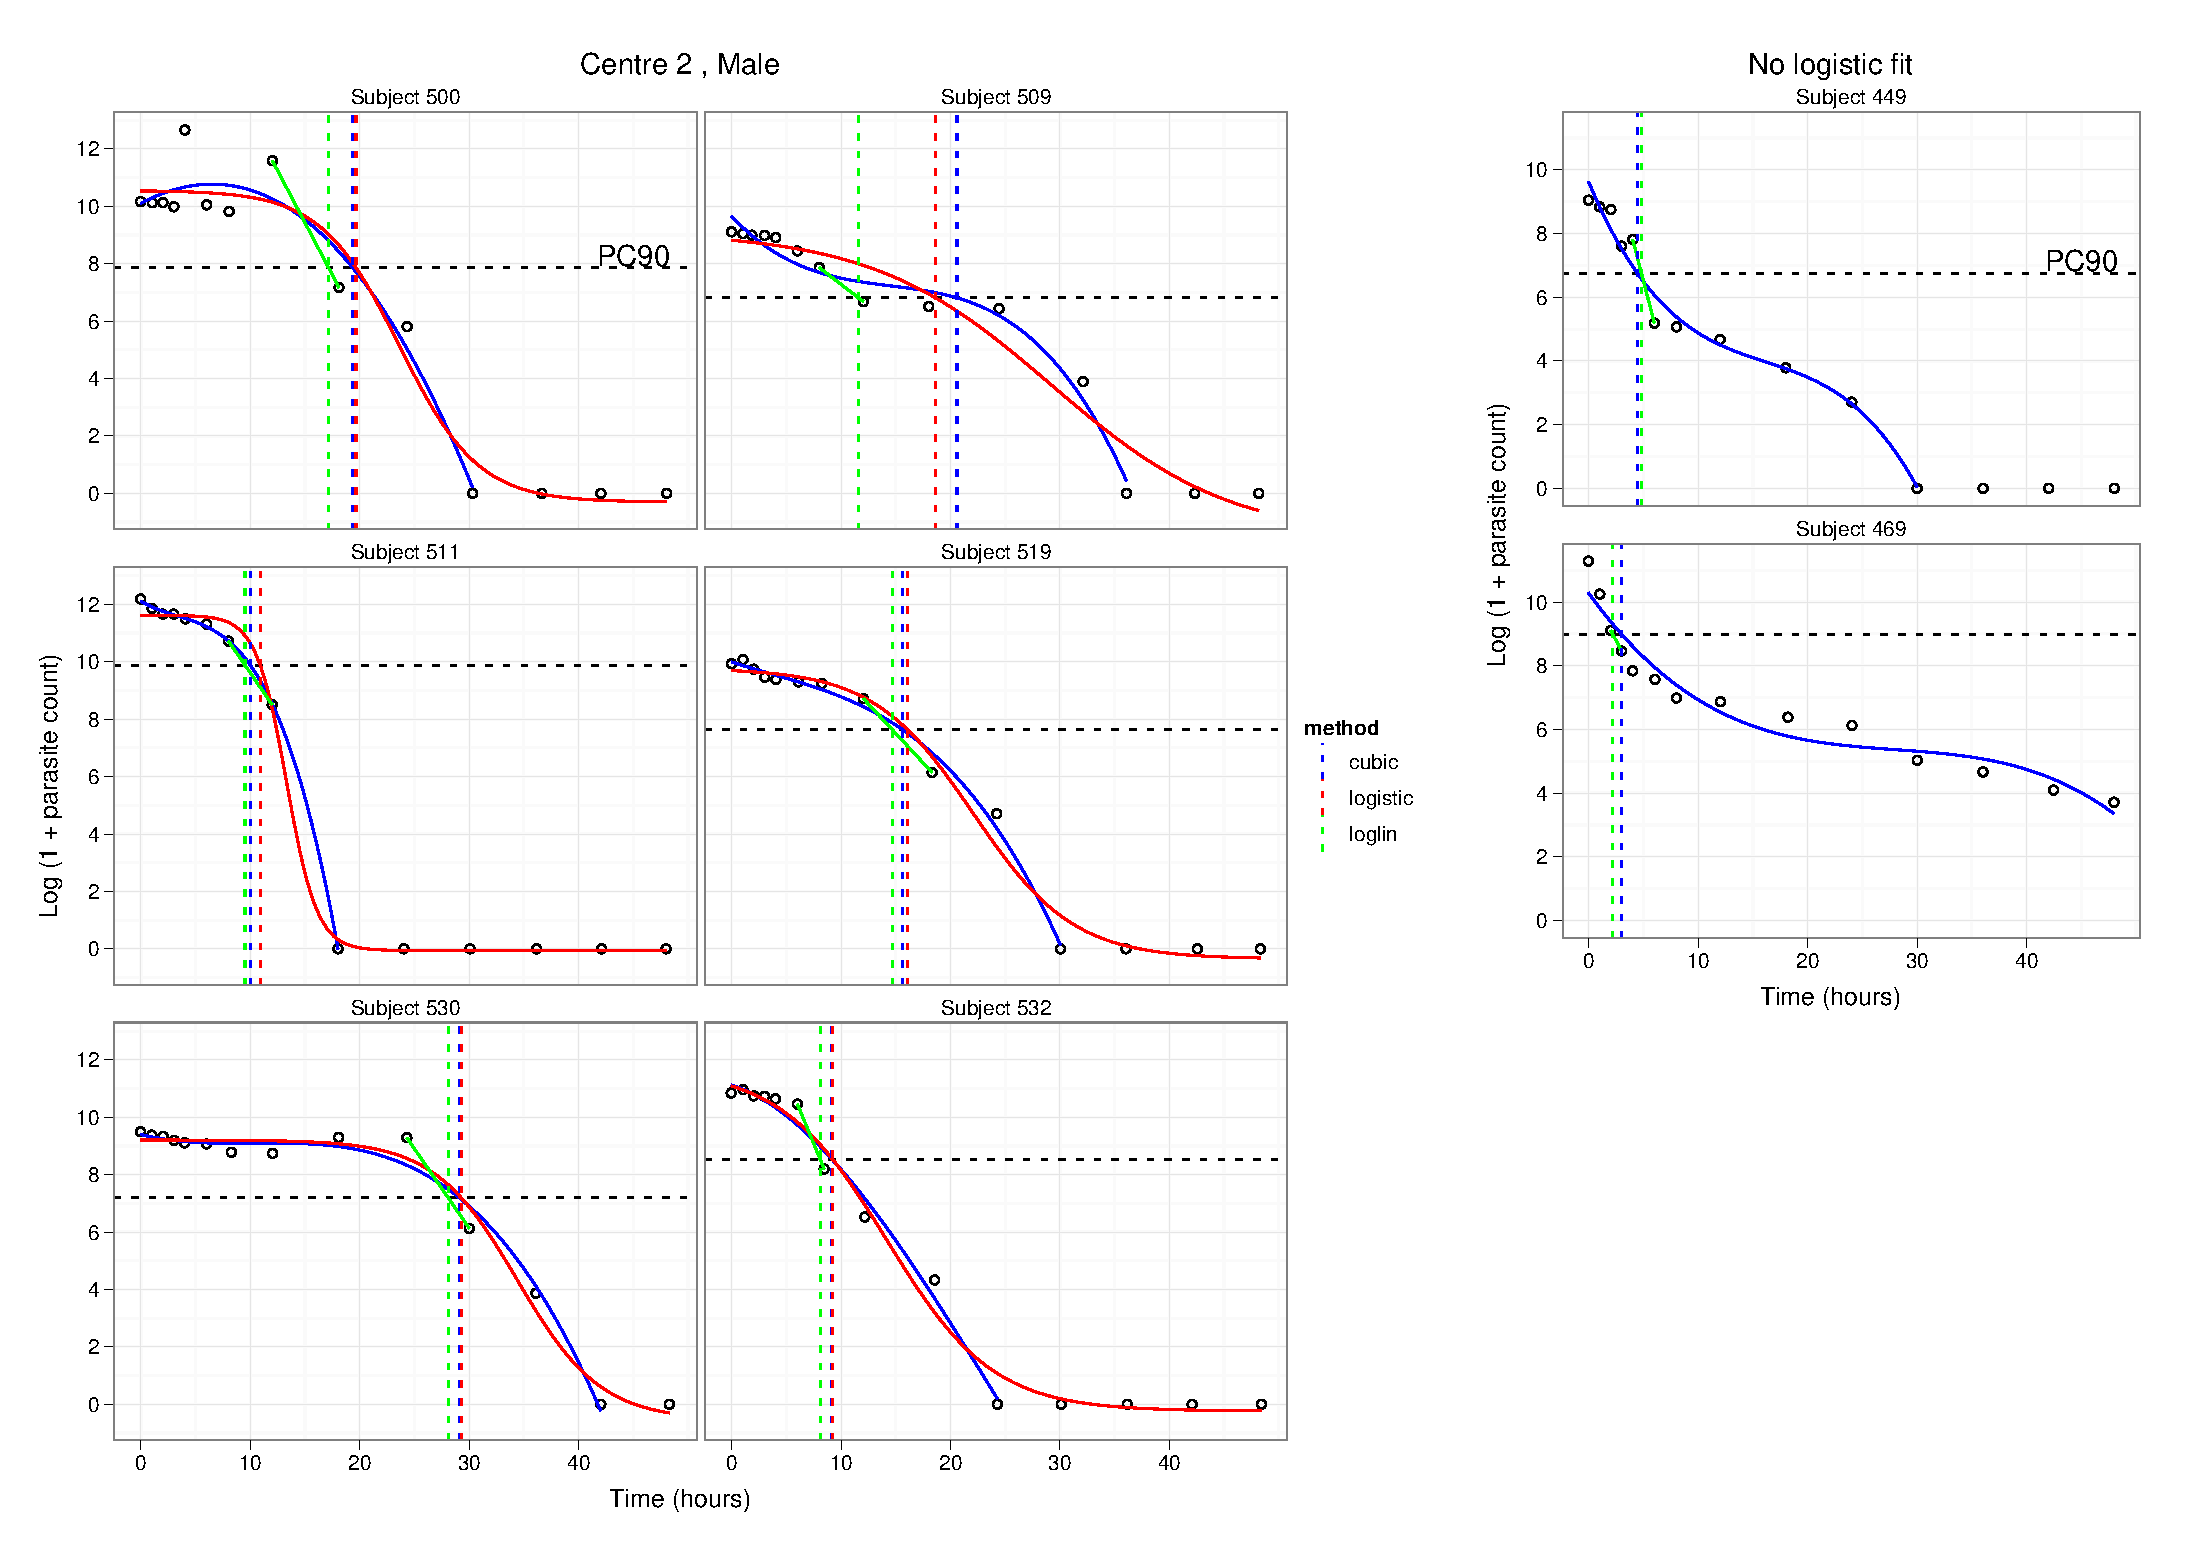
\includegraphics[height=150mm]{Afits2M.eps}
\end{sidewaysfigure}
\begin{sidewaysfigure}
\centering
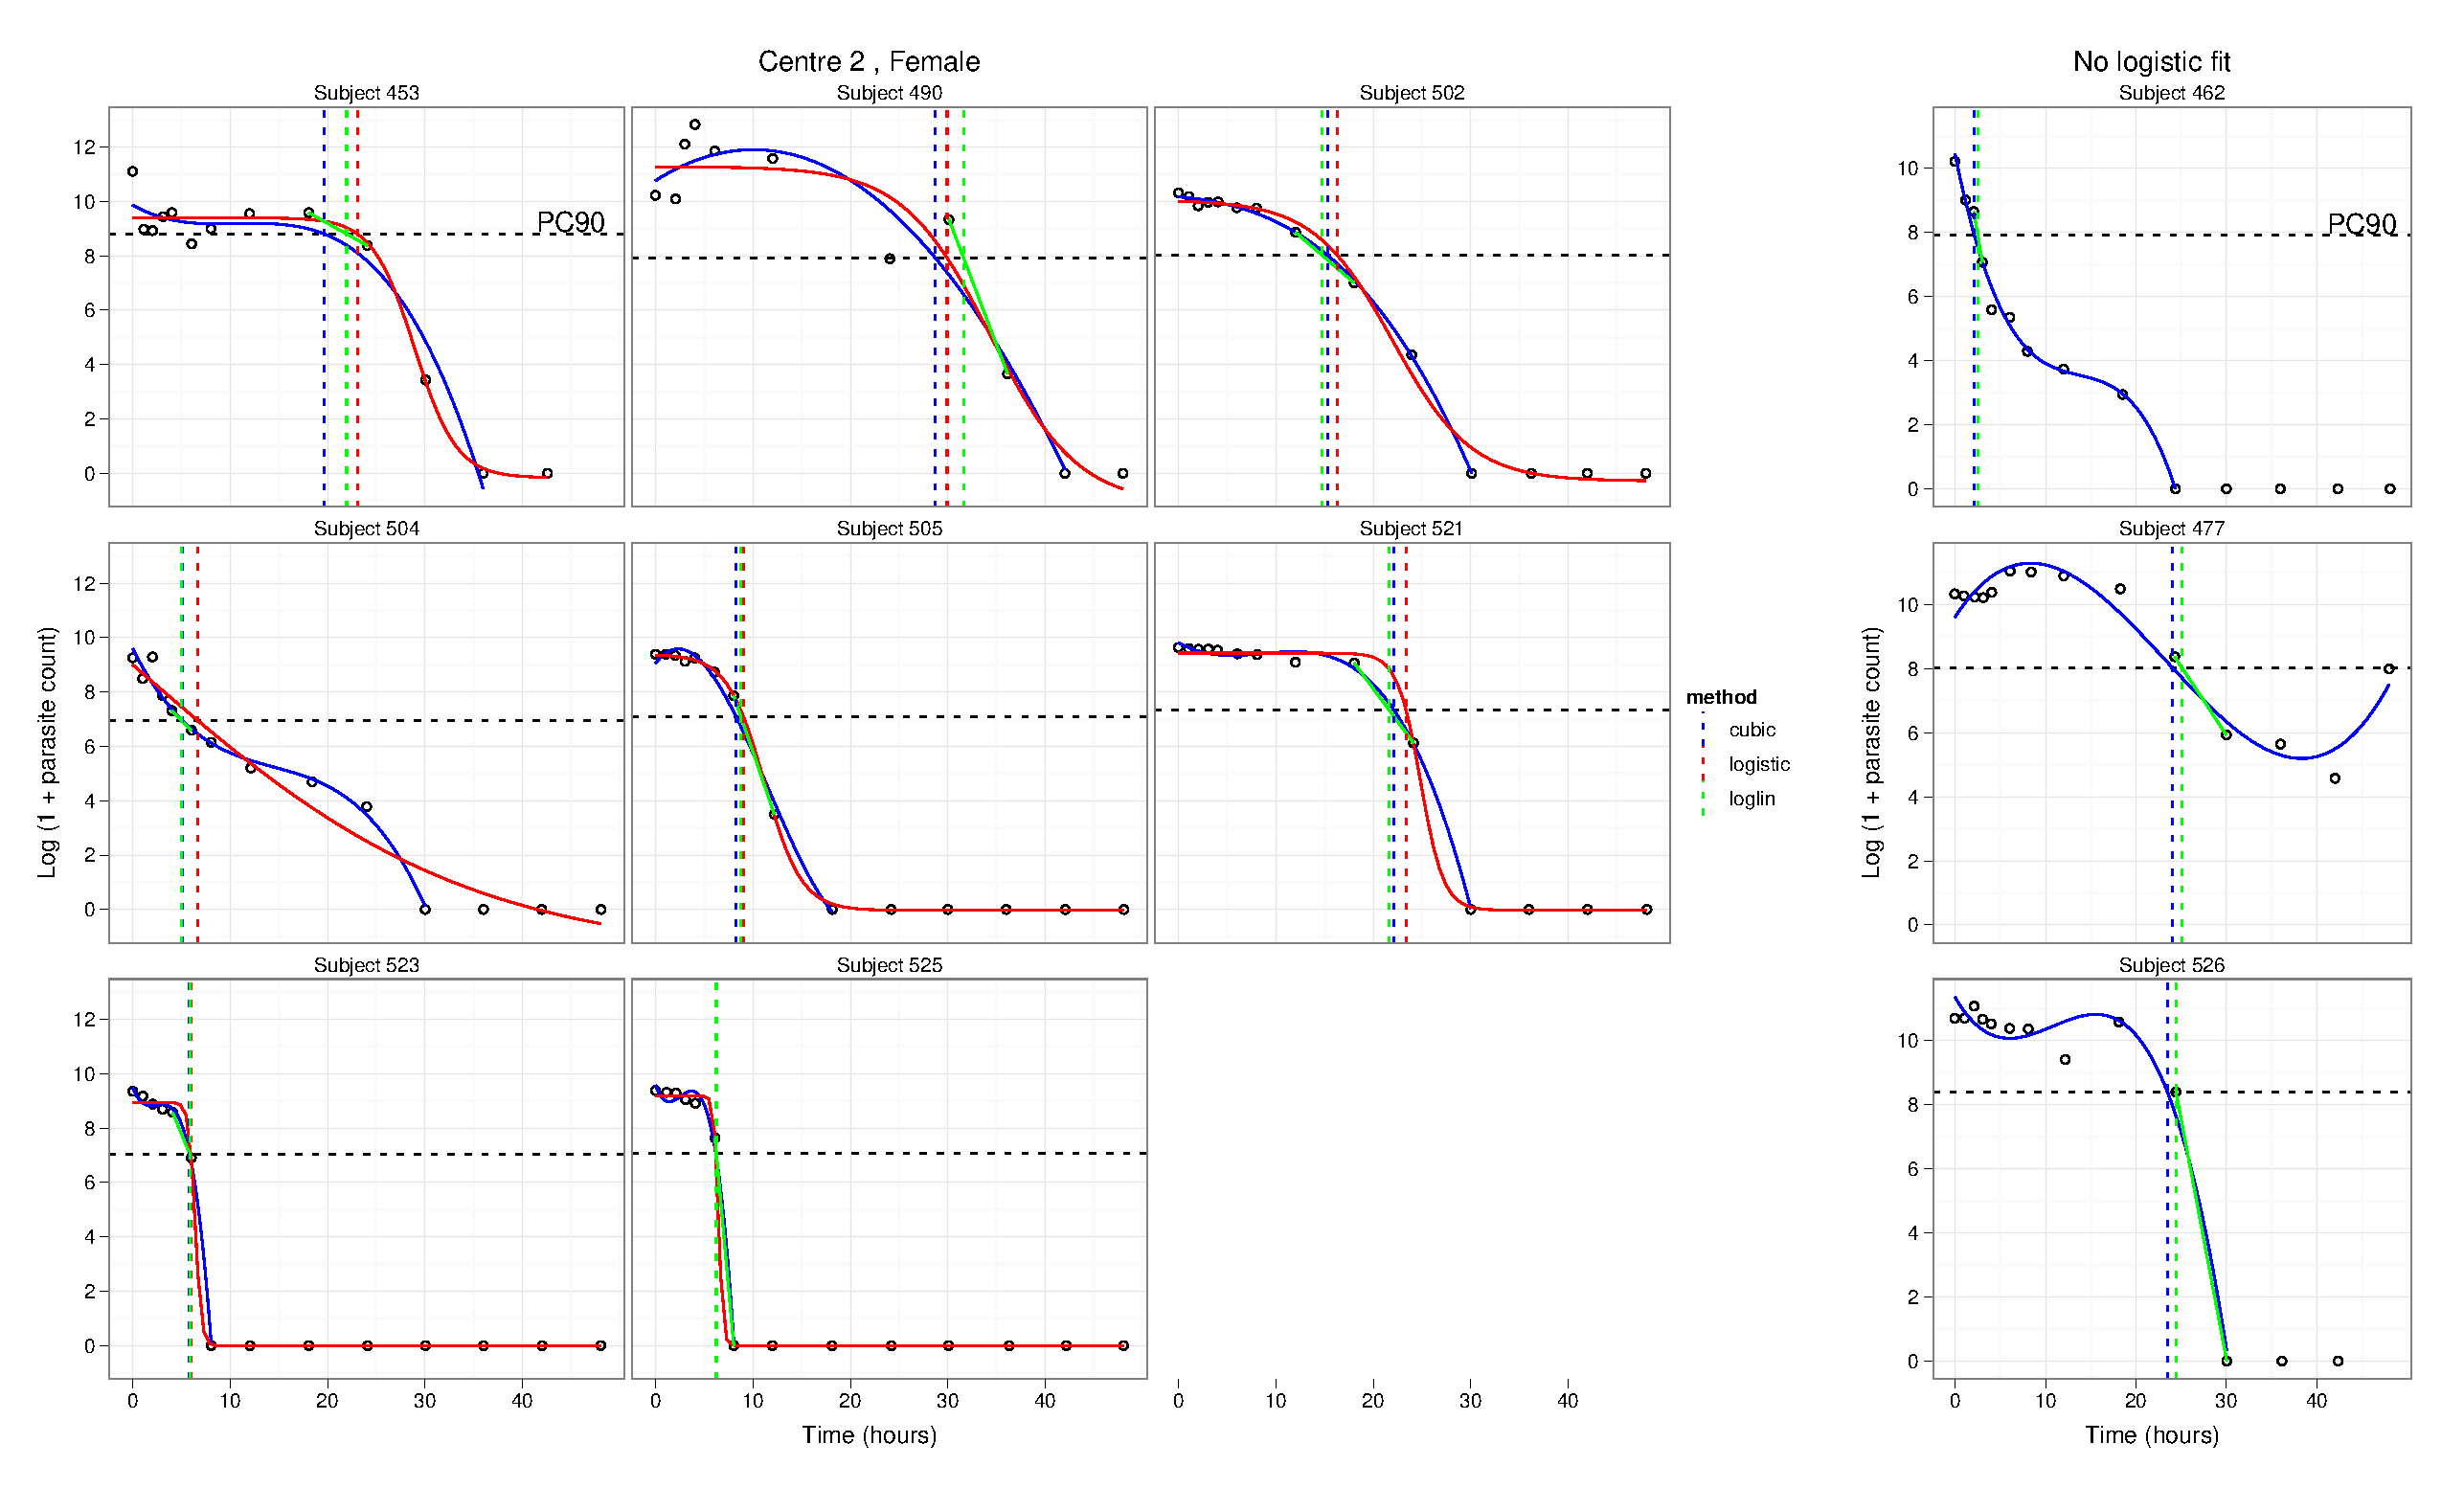
\includegraphics[height=150mm]{Afits2F.eps}
\end{sidewaysfigure}

\chapter{\emph{R} code listings}
\lstset{numberstyle=\small,
frame=single,
framesep=6pt,
tabsize=2,
basicstyle=\small\ttfamily,
%breakautoindent=false,
%breakindent=0pt,
%keywordstyle=\bfseries,
%keywordstyle=\color{blue},
%commentstyle=\itshape\color{red},
showstringspaces=false,
columns = fullflexible,
language=R,
breaklines=true,
showstringspaces=false,
lineskip=-1pt}

This appendix contains a subset of the \emph{R} code written for this dissertation. The code to show the key algorithms used in numerical calculations is shown and a sample of plotting routines to demonstrating how some of the figures in this dissertation were created.

\section{Functions for PC90 estimation}\label{R:PC90}
\begin{lstlisting}[caption=Functions to find PC90 by cubic regression,label=R:cubics]
# Create a list of cubic fits to data up to first zero
cubic.fits <- function(data) {
	require(nlme)
	lmList(log(1 + parct) ~ acttm + I(acttm^2) + I(acttm^3) | SUBJID, data=uptofirstzero(data))
}

# Create a new data frame containing data up to first zero count
uptofirstzero <- function(data) {
	new.df <- data.frame()
	for (s in unique(data$SUBJID)) {
		rows <- data[data$SUBJID==s,]
		n <- match(0, rows$parct)
		if (!is.na(n)) {
			rows <- rows[1:n,]
		}
		new.df <- rbind(new.df, rows)
	}
	new.df
}


# Find the PC90 time from a cubic fit
pc90cubic <- function(fit, data) {
	coefs <- coef(fit)
	parct90 <- log(1 + (data$parct[data$plantm=='PRE-DOSE'] * 0.1))
	preds <- predict(fit)
	
	# Find the times at which counts are above and below PC90 
	upper <- which.min(preds > parct90)
	lower <- upper - 1
	interval <- c(data$acttm[lower], data$acttm[upper])

	# Search for PC90 between these times
	soln <- uniroot(function(x) coefs[1] + coefs[2]*x + coefs[3]*x^2 + coefs[4]*x^3 - parct90, interval=interval)
	soln$root
}
\end{lstlisting}

\begin{lstlisting}[caption=Functions to find PC90 by logistic regression,label=R:logistics]
# Perform logistic fitting after selecting starting parameters
logistic.fit <- function(dat) {
	# Set alpha and lambda to max and min counts
	initA <- max(log(1 + dat$parct))
	initL <- min(log(1 + dat$parct))

	# Set mu to time closest to half max count
	halfway <- (initA + initL)/2
	initU <- dat$acttm[which.min(abs(log(1 + dat$parct) - halfway))]

	# Set beta to -0.5 i.e. 2 in SSfpl formulation
	initB <- 2
	
	tryCatch(fit <- nls(log(1 + parct) ~ SSfpl(acttm, A, L, U, B), data=dat,
				start=list(A=initA, L=initL, U=initU, B=initB)),
		error=function(e) e)
	fit
}

# Find PC90 time from logistic fit
getPC90.logistic <- function(fit, data) {
	parct90 <- log(1 + (data$parct[data$plantm=='PRE-DOSE'] * 0.1))
	preds <- predict(fit)

	# Find the times at which counts are above and below PC90
	upper <- which.min(preds > parct90)
	lower <- upper - 1
	interval <- c(data$acttm[lower], data$acttm[upper])

	# Search for PC90 between these times
	soln <- uniroot(function(x) predict(fit, data.frame(acttm=x)) - parct90, interval=interval)
	soln$root
}
\end{lstlisting}

\begin{lstlisting}[caption=Functions to find PC90 by log-linear interpolation,label=R:loglinear]
# Get PCx time from log-linear interpolation
getPC.loglin <- function(data, PC=90) {
	pc <- log(1 + (data$parct[data$plantm=='PRE-DOSE'] * (100 - PC)/100))
	fit <- lmloglin(data, PC)
	B0 <- coef(fit)[1]
	B1 <- coef(fit)[2]
	(pc - B0) / B1
}

# Perform linear fit between two points either side of PCx
lmloglin <- function(data, PC=90) {
	lm(log(1 + parct) ~ acttm, data=data, subset=getAboveBelow(data, PC))
}

# Get indices of counts immediately above and below PCx level
getAboveBelow <- function(data, PC=90) {
	pc90 <- data$parct[data$plantm=='PRE-DOSE'] * (100 - PC)/100
	above.pc90 <- which(data$parct > pc90)
	upper <- above.pc90[length(above.pc90)]
	lower <- upper + 1
	c(upper, lower)
}
\end{lstlisting}

\section{Resampling functions}\label{R:resamp}
\begin{lstlisting}[caption=Functions for resampling $F$ statistic,label=R:Fresamp]
# Resample the F statistic by permutation
resample.aov <- function(fit, n=1000, bootstrap=F) {
	model.terms <- attr(terms(fit), "term.labels")
	p <- length(model.terms)
	F.samples <- matrix(nrow=n, ncol=p, dimnames=list(sample=1:n, term=model.terms))
	data <- fit$model
	response.sample <- data[,1]

	F.values <- summary(fit)[[1]][4]
	F.samples[1,] <- F.values[1:p,1]
	for (i in 2:n) {
		data[,1] <- sample(response.sample, length(response.sample), replace=bootstrap)
		fit.resample <- update(fit, data=data)
		F.values <- summary(fit.resample)[[1]][4]
		F.samples[i,] <- F.values[1:p,1]
	}
	F.samples	
}

# Restricted resampling of F statistic by strata
restricted.resample.aov <-  function(fit, strata, n=1000, bootstrap=F) {
	model.terms <- attr(terms(fit), "term.labels")
	p <- length(model.terms)
	F.samples <- matrix(nrow=n, ncol=p, dimnames=list(sample=1:n, term=model.terms))
	data <- fit$model
	randomize.within <- lapply(strata, function(x) data[,x])

	F.values <- summary(fit)[[1]][4]
	F.samples[1,] <- F.values[1:p,1]
	for (i in 2:n) {
		resample.list <- as.list(by(data, randomize.within, function(x) {
			x[,1] <- sample(x[,1], length(x[,1]), replace=bootstrap)
			x
		}))
		for (strata.sample in resample.list) {
			data[dimnames(strata.sample)[[1]],] <- strata.sample
		}
		# Checksum on strata for code verification
		# by(data, randomize.within, function(x) print(sum(x$PC90.loglin)))
		fit.resample <- update(fit, data=data)
		F.values <- summary(fit.resample)[[1]][4]
		F.samples[i,] <- F.values[1:p,1]
	}
	F.samples	
}
\end{lstlisting}

\begin{lstlisting}[caption=Functions to calculate resampled $p$-values and resampling residuals,label=R:resampmisc]
# Calculate resampled p-values
pf.resample <- function(fit, n=1000, bootstrap=F) {
	F.samples <- resample.aov(fit, n, bootstrap)
	p <- dim(F.samples)[2]
	F.actual <- summary(fit)[[1]][4][1:p,1]
	indicators <- apply(F.samples, 1, function(x) x > F.actual)
	t(t(rowMeans(indicators)))
}

# Calculate Still and White residuals
stillwhite.resid <- function(row, data) {
	centre <- row['Centre'][1,1]
	sex <- row['Sex'][1,1]
	trt <- row['Treatment'][1,1]
	Xcst <- row['PC90'][1,1]
	Xstar <- with(data, Xcst - mean(PC90[Centre==centre]) - mean(PC90[Sex==sex]) - mean(PC90[Treatment==trt]) + mean(PC90))
	Xstar
}
\end{lstlisting}

\begin{lstlisting}[caption=Functions to calculate confidence intervals by resampling,label=R:resampCI]
# Find CIs by resampling
resample.ci <- function(k, R=1000) {
	with(PC90.df[PC90.df$Sex=='Female',], t.resample(PC90.loglin[Treatment=='alone'] - k, PC90.loglin[Treatment=='combi'], R))
}

# Resample t statistic
t.resample <- function(x1, x2, R=1000, bootstrap=F) {
	Tobs <- mean(x1) - mean(x2)
	n1 <- length(x1)
	n2 <- length(x2)
	values <- c(x1, x2)
	n <- length(values)
	values.resampled <- replicate(R - 1, sample(values, n, replace=bootstrap))
	T <- c(Tobs, apply(values.resampled, 2, function(x) mean(x[1:n1]) - mean(x[n1+1:n2])))
	mean(abs(T) > abs(Tobs))
}
\end{lstlisting}

\section{Functional data analysis}\label{R:fda}
\begin{lstlisting}[caption=Functions for cubic spline smoothing,label=R:fdsmooth]
# Get spline basis, cubic by default
getBasis <- function(knots, norder=4) {
	require(fda)
	nbasis <- length(knots) + norder - 2
	create.bspline.basis(range(knots), nbasis, norder, knots)
}

# Get spline smoothed functional data
getFdsmooth <- function(x, y, smoothing=10) {
	# x <- malaria.fda.df$pt
	cubic.basis <- getBasis(x)
	cubic.fdPar <- fdPar(cubic.basis, 2, smoothing)
	# y <- as.matrix(malaria.fda.df$lparct)
	smooth.basis(x, y, cubic.fdPar)
}
\end{lstlisting}

Some of the code in the following listings is based on examples from Giles Hooker's Applied Functional Data Analysis course at Cornell University.\\
\url{http://www.bscb.cornell.edu/~hooker/FDA2008/}
\begin{lstlisting}[caption=Functions for fda regression,label=R:fregress]
# Perform regression
getfRegress <- function(data.smooth, smoothing=10) {
	require(fda)

	fd <- data.smooth$fd
	x <- data.smooth$argvals
	y <- data.smooth$y

	# Get the factors as a list of fda objects
	xfdlist <- getxfdlist()
	# Get the coefficient fdas to be fitted
	betalist <- getbetalist(fd, smoothing)

	# Do the regression and add the standard errors for the coefficients
	fr <- fRegress(fd, xfdlist, betalist, y2cMap=data.smooth$y2cMap)
	fr$SigmaE <- getSigmaE(fr, x, y)
	fr$betastderrlist <- getfStderr(fr, x, y)$betastderrlist
	fr
}

# Get factor fdas for regression
getxfdlist <- function() {
	pt.cbasis <- create.constant.basis(range(malaria.fda.df$pt))
	constfd=fd(matrix(1, 1, 43), pt.cbasis)
	Sexfd=fd(matrix(as.numeric(malaria.fda.df$Sex) - 1, 1, 43), pt.cbasis)
	Treatmentfd=fd(matrix(as.numeric(malaria.fda.df$Treatment) - 1, 1, 43), pt.cbasis)
	Interactionfd=fd(matrix((as.numeric(malaria.fda.df$Sex) - 1)*(as.numeric(malaria.fda.df$Treatment) -1), 1, 43), pt.cbasis)
	list(constfd, Sexfd, Treatmentfd, Interactionfd)
}

# Get paramater fdas for regression
getbetalist <- function(fd, smoothing=10) {
	betaifdPar <- fdPar(fd$basis, 2, smoothing)
	list(betaifdPar, betaifdPar, betaifdPar, betaifdPar)
}

# Get var-covar matrix
getSigmaE <- function(fit, x, y) {
	yobs <- eval.fd(x, fit$yhatfdobj$fd)
	e <- y - yobs
	e %*% t(e) / dim(y)[2]
}

# Get the standard error of the coefficients
getfStderr <- function(fit, x, y) {
	sigmaE <- getSigmaE(fit, x, y)
	fRegress.stderr(fit, fit$y2cMap, sigmaE)
}
\end{lstlisting}

\begin{lstlisting}[caption=Functions to calculate fda regression standardized residuals and confidence intervals for fitted values,label=R:fdaresid]
# Get the standardized residuals for fda regression
getfResid <- function(fit, data.smooth) {
	x <- data.smooth$argvals
	n <- dim(data.smooth$y)[2]
	errmat <- data.smooth$y - eval.fd(x, fit$yhatfdobj$fd)
	resids.df <- data.frame(pt=x, as.data.frame(errmat))
	p <- n + 1
	resids.long <- reshape(resids.df, direction='long', varying=list(2:p))
	names(resids.long)[2:3] <- c("Subject","e")
	resids.long$s <- rep(sqrt(diag(fit$SigmaE)), n)
	resids.long$sr <- with(resids.long, e/s)
	resids.long$Sex <- factor("Male","Female")
	resids.long$Treatment <- factor("alone","combi")
	for (i in 1:n) {
		resids.long$Sex[resids.long$Subject==i] <- PC90.df$Sex[PC90.df$Subject==i]
		resids.long$Treatment[resids.long$Subject==i] <- PC90.df$Treatment[PC90.df$Subject==i]
	}
	resids.long
}

# Calculate confidence intervals for fitted fda mean function
getfdpred <- function(t, fit, conf=0.95) {
	require(fda)

	# Get matrix of factor levels for each sex/treatment group
	x <- t(sapply(getPredxfdlist(), function(x) x$coef))
	# Get vector of coefficients
	Beta <- as.matrix(sapply(fit$betaestlist, function(x) eval.fd(t, x$fd)))
	# Get fitted values
	pred <- t(x) %*% Beta

	# Calculate residuals and residual variance
	yobs <- eval.fd(fit$yfdPar$fd, t)
	yfit <- eval.fd(fit$yhatfdobj$fd, t)
	e <- yobs - yfit
	n <- length(e)
	p <- length(Beta)
	s2 <- e %*% t(e) / (n - p)

	# Calculate variance of predictions
	X <- model.matrix(fit)
	varpred <- as.numeric(s2) * t(x) %*% solve(t(X) %*% X) %*% x

	# Return predictions at times specified with CIs specified
	pval <- (1 - conf) / 2
	limit <- sqrt(diag(varpred)) * abs(qt(pval, n - p))
	matrix(c(rep(t, p), pred, pred-limit, pred+limit), p, p,
		dimnames=list(NULL, c("t", "pred", "lwr", "upr")))
}
\end{lstlisting}

\section{Plotting functions}\label{R:plot}
The figures in this dissertation were plotted using Hadley Wickham's \texttt{ggplot2} \emph{R} library.\\
\url{http://had.co.nz/ggplot2/}
\begin{lstlisting}[caption=Plot raw count data for male and female subjects side-by-side,label=R:rawggplot]
# Plot raw data for male and female subjects side-by-side
rawggplot3 <- function(data, title="", centre="", r1=4, r2=4, points=T, lines=T) {
	require(ggplot2)

	vp1 <- viewport(width=0.45, x=0, just="left")
	q <- getrawplot(data[data$SEX=='Male',])
	q <- addtrtgeoms(q, points, lines)
	q <- q + opts(title=paste(centre, "Male"), legend.position='none')
	q <- q + facet_wrap(~SUBJID, nrow=r1, scales="free_y")
	print(q, vp=vp1)

	vp2 <- viewport(width=0.55, x=1, just="right")
	q <- getrawplot(data[data$SEX=='Female',])
	q <- addtrtgeoms(q, points, lines)
	q <- q + opts(title=paste(centre, "Female"))
	q <- q + facet_wrap(~SUBJID, nrow=r2, scales="free_y")
	print(q, vp=vp2)
}

# Set up the basic plot with data, scales and panels by subject
getrawplot <- function(data) {
	q <- ggplot(data, aes(x=acttm, y=parct))
	q <- q + scale_x_continuous(name="Time (hours)")
	q <- q + scale_y_continuous(formatter=function(x) return(x/1000), name="Parasite Count (1000s)")
	l <- length(unique(data$SUBJID))
	q + facet_wrap(~SUBJID, ncol=min(3,l), scales="free_y")
}

# Change point shape and line colour to reflect treatment group
addtrtgeoms <- function(q, points=T, lines=T) {
	# Reorder the patient factor so that "alone" treatment patients are first
	for(subj in as.character(unique(q$data$SUBJID[q$data$trt=='A']))) {
		q$data$SUBJID <- relevel(q$data$SUBJID, subj)
	}
	if (points) {
		q <- q + geom_point(aes(shape=trttxt, colour=trttxt))
	}
	if (lines) {
		q <- q + geom_line(aes(colour=trttxt))
	}
	q + scale_shape(name="Treatment") + scale_colour_discrete("Treatment")
}
\end{lstlisting}

\begin{lstlisting}[caption=Boxplots of pre-dose count by sex\, centre and treatment,label=R:predoseaov]
# Plot pre-dose counts as boxplots by centre, sex and treatment
predoseaov2 <- function(data) {
	require(ggplot2)

	# Boxplots of pre-dose count by sex for each centre
	vp1 <- viewport(width=1, height=0.33, y=1, just="top")
	q1 <- qplot(SEX, parct, data=data, geom="blank", colour=SEX, xlab="Sex:Centre", ylab="")
	q1 <- q1 + scale_colour_discrete(h.start=120)
	q1 <- q1 + scale_y_continuous(limits=c(0,100000), formatter="comma")
	q1 <- q1 + geom_boxplot(width=0.3, outlier.size=0)
	q1 <- q1 + geom_point(position=position_jitter(w=0.1))
	q1 <- q1 + opts(legend.position="none")
	q1 <- q1 + facet_grid(.~CENTREID)
	print(q1, vp=vp1)

	# Boxplots of pre-dose count by treatment for each centre
	vp2 <- viewport(width=1, height=0.33, y=0.5, just="centre")
	q2 <- qplot(trttxt, parct, data=data, geom="blank", colour=trttxt, xlab="Treatment:Centre", ylab="Parasite Count")
	q2 <- q2 + scale_y_continuous(limits=c(0,100000), formatter="comma")
	q2 <- q2 + geom_boxplot(width=0.3, outlier.size=0)
	q2 <- q2 + geom_point(position=position_jitter(w=0.1))
	q2 <- q2 + opts(legend.position="none")
	q2 <- q2 + facet_grid(.~CENTREID)
	print(q2, vp=vp2)

	# Boxplots of pre-dose count by treatment for each sex
	vp3 <- viewport(width=1, height=0.33, y=0, just="bottom")
	q3 <- qplot(trttxt, parct, data=data, geom="blank", colour=trttxt, xlab="Treatment:Sex", ylab="")
	q3 <- q3 + scale_y_continuous(limits=c(0,100000), formatter="comma")
	q3 <- q3 + geom_boxplot(width=0.3, outlier.size=0)
	q3 <- q3 + geom_point(position=position_jitter(w=0.1))
	q3 <- q3 + opts(legend.position="none")
	q3 <- q3 + facet_grid(.~SEX)
	print(q3, vp=vp3)
}
\end{lstlisting}

\begin{lstlisting}[caption=Residuals diagnostic plots for \texttt{lm,aov} fitted models,label=R:plotresids.lm]
# Residuals diagnostics plots for lm/aov fit
plotresids.lm <- function(model, resids, data, binwidth=0.5, trans=F, weighted=F, xlab="Fitted PC90 (hours)") {
	require(ggplot2)
	require(MASS)
	if (missing(resids)) {
		resids <- stdres(model)
	}
	if (missing(data)) {
		data <- model$model
	}
	lab.txt <- "Standardized residuals"

	# Histogram
	vp1 <- viewport(width=0.5, height=0.5, x=0.25, y=0.75)
	q <- qplot(resids, xlab=lab.txt, geom="blank") + geom_histogram(colour="black", fill="white", binwidth=binwidth) 
	print(q, vp=vp1)

	# QQ normal
	vp2 <- viewport(width=0.5, height=0.5, x=0.75, y=0.75)
	q <- qplot(sample=resids)
	y <- quantile(resids, c(0.25, 0.75))
	x <- qnorm(c(0.25, 0.75))
	slope <- diff(y)/diff(x)
	int <- y[1L] - slope * x[1L]
	q <- q + geom_abline(intercept=int, slope=slope, linetype=2)
	print(q, vp=vp2)

	# vs factors
	vp3 <- viewport(width=0.5, height=0.5, x=0.25, y=0.25)
	p <- dim(data)[2] - weighted
	data.l <- reshape(data, direction="long", varying=list(2:p), v.names="Factor")
	if (p > 2)
		q <- qplot(Factor, rep(resids, p-1), data=data.l, geom="blank", ylab=lab.txt, colour=time)
	else
		q <- qplot(Factor, resids, data=data.l, geom="blank", ylab=lab.txt)
	q <- q + geom_hline(aes(yintercept=0), linetype=2)
	q <- q + geom_point(position=position_jitter(w=0.1))
	if (is.factor(data$Factor))
		q <- q + stat_summary(fun.dat="mean_sdl", mult=1, geom="crossbar", width=0.5)
	q <- q + opts(legend.position="none")
	print(q, vp=vp3)

	# vs fitted
	vp4 <- viewport(width=0.5, height=0.5, x=0.75, y=0.25)
	q <- qplot(fitted(model)^(1+1*trans), resids, data=data, xlab=xlab, ylab=lab.txt)
	q <- q + geom_hline(aes(yintercept=0), linetype=2)
	print(q, vp=vp4)
}
\end{lstlisting}

\begin{lstlisting}[caption=Plot all 3 PC90 methods on same plot,label=R:comparePC90]
# All 3 PC90 estimation methods on same plot
comparePC90 <- function(dat, pc90, logfit=T, ...) {
	q <- getrawplot(dat) + geom_point(shape=1)
	q <- getlogplot(q)
	q <- addPC90lines(q, logplot=T)
	q <- addcubicfit(q, colour="blue")
	if (logfit) {
		tryCatch(q <- addlogfit(q, colour="red", ...), error=function(e) {})
	}
	q <- addloglin(q, colour="green")
	addPC90vlines(q, pc90) + facet_wrap(~SUBJID, ncol=2)
}

# Convert the plot q to log-linear
getlogplot <- function(q) {
	q <- q %+% transform(q$data, parct=log(1+parct))
	q <- q + scale_y_continuous(name="Log (1 + parasite count)")
	l <- length(unique(q$data$SUBJID))
	q + facet_wrap(~SUBJID, ncol=min(3,l), scales="fixed")
}

# Add cubic fit to plot q
addcubicfit <- function(q, ...) {
	q + stat_smooth(method="lm", formula=y~x+I(x^2)+I(x^3), data=uptofirstzero(q$data), fullrange=F, se=F, ...) 
}

# Add logistic fit to plot q
addlogfit <- function(q, ...) {
	q + stat_smooth(method="nls", formula="y ~ SSfpl(x, A, L, U, B)", se=F, ...)
}

# Add log-linear interpolation to plot q
addloglin <- function(q, ...) {
	dat <- q$data
	dat$parct <- exp(q$dat$parct) - 1
	dat <- by(dat, dat$SUBJID, getAboveBelow)
	data <- data.frame()
	for (s in unique(q$data$SUBJID)) {
		data <- rbind(data, q$data[q$data$SUBJID==s,][dat[[s]],])
	}
	q + geom_line(data=data, ...)
}

# Add vertical lines showing 3 PC90 estimates
addPC90vlines <- function(q, dat, colours=c("blue", "red", "green")) {
	dat <- subset(dat, subset=SUBJID %in% unique(q$data$SUBJID))
	q + geom_vline(data=dat, aes(xintercept=PC90, colour=method), linetype=2) + scale_colour_manual(values=colours)
}
\end{lstlisting}

\begin{lstlisting}[caption=Functional data analysis plots,label=R:fdaplot]
# Plot coefficients from fda regression with CIs
plotfdcoefs <- function(fit, nx=201) {
	require(fda)
	require(ggplot2)
	
	rngx <- fit$yfdPar$fd$basis$range
	x <- seq(rngx[1], rngx[2], length=nx)
	coef.names <- c("Mean (male, alone)", "Sex (female)", "Treatment (combi)", "Sex:Treatment (female, combi)")
	plot.df <- data.frame()
	for (i in 1:4) {
		y <- eval.fd(x, fit$betaestlist[[i]]$fd)
		s <- eval.fd(x, fit$betastderrlist[[i]])[,1]
		plot.df <- rbind(plot.df, data.frame(x=x, y=y, upper=y+1.96*s, lower=y-1.96*s, coef=coef.names[i]))
	}
	q <- qplot(x, y, data=plot.df, geom='line', colour=coef, size=1, xlab="Time (hours)", ylab="log ratio of parasite count to pre-dose", main="Fitted coefficient functions with 95% confidence intervals")
	q <- q + geom_line(aes(y=upper), linetype=2) + geom_line(aes(y=lower), linetype=2)
	q <- q + geom_hline(yintercept=0, linetype=2)
	q + facet_wrap(~coef, ncol=2) + opts(legend.position='none')
}

# Plot F statistic fda
plotFperm <- function(fperm, x, y1, y2) {
	require(ggplot2)
	
	time <- fperm$argvals
	q <- qplot(time, fperm$Fvals, colour='red', size=1, geom='line', xlab='Time (hours)', ylab='F-statistic', main='Permutation F-test')
	q <- q + geom_line(aes(y=fperm$qvals.pts), linetype=3, colour='blue')
	q <- q + geom_hline(yintercept=fperm$qval, linetype=2, colour='blue')
	q <- q + geom_text(aes(x=x, y=y1, label="maximum 0.05 critical value"), size=4, colour='blue')
	q <- q + geom_text(aes(x=x, y=y2, label="pointwise 0.05 critical value"), size=4, colour='blue')
	q + opts(legend.position='none')
}


# Get data for plotting predictions and CIs over time range
getfdpreddata <- function(fit, nt=201, level.names=c("Male, alone", "Female, alone", "Male, combi", "Female, combi")) {
	rngt <- fit$yfdPar$fd$basis$range
	t <- seq(rngt[1], rngt[2], length=nt)
	data.df <- data.frame(getfdpred(t[1], fit))
	for (i in 2:nt)
		data.df <- rbind(data.df, getfdpred(t[i], fit))
	data.df$level <- rep(level.names, nt)
	data.df
}

# Plot fitted function with CIs
plotfdpred <- function(data) {
	require(ggplot2)
	q <- qplot(t, pred, data=data, ymin=lwr, ymax=upr, geom='errorbar', colour=Treatment, xlab="Time (hours)", ylab="log ratio of parasite count to predose", main="95% confidence intervals for functional model")
	#q + geom_line(aes(y=lwr), linetype=2) + geom_line(aes(y=upr), linetype=2)
	#q + geom_errorbar(aes(ymin=lwr, ymax=upr, colour=Treatment))
	q <- q + geom_line(size=1)
	q + facet_grid(~Sex)
}
\end{lstlisting}

%\begin{lstlisting}[language=SAS,caption=SAS,label=SAS]
%data subjects;
%	set Project.Msc_data;
%	x=acttm;
%	y=log(1+parct);
%	run;
%data predose;
%	set Project.Msc_data (keep=SUBJID plantm parct);
%	if plantm eq 'PRE-DOSE';
%	l90 = log(1 + (0.1 * parct));
%	run;	
%proc nlin data=subjects;
%	parms A=0 to 12 L=8 to 14 B=-0.5 to 0 by 0.1  U=5 to 20 by 5;
%	model y=A+(L/(1+exp(-B*(x-U))));
%	by SUBJID;
%	output out=nlinfit p=pred;
%	run;
%quit;
%data plotdata;
%	merge nlinfit predose;
%	by SUBJID;
%	run;
%symbol1 c=black i=none v=x;
%symbol2 c=blue i=join v=none;
%symbol3 c=black i=join l=2 v=none;
%proc gplot data=plotdata;
%	plot (y pred l90)*x / overlay;
%	by SUBJID;
%	run;
%quit;
%\end{lstlisting}
\end{singlespace}

\backmatter
\bibliographystyle{wileyj}
\renewcommand{\bibname}{References}
{\singlespace\bibliography{dissertation}}
\end{document}